\documentclass[10pt,a4paper,twoside]{article} 
\usepackage[latin1]{inputenc}
\usepackage[english]{babel}
\usepackage{amsmath}
\usepackage{amsfonts}
\usepackage{amssymb}
\usepackage{makeidx}
\usepackage{graphicx}
\usepackage{hyperref}
\usepackage[left=2cm,right=2cm,top=2cm,bottom=2cm]{geometry}
\usepackage{float}
\usepackage{multirow}
\usepackage{verbatim} %for å kommentere ut ting
\usepackage[nottoc,numbib]{tocbibind}

\raggedbottom

%ræl som trengs for bibliografi
%\usepackage{splitbib} %bibliografi seksjon

%\begin{category}[]{Periodicals}
%\SBentries{bib:SF6PI,bib:AFIMVLBA,bib:CIAMVLBS,bib:StatSF6,bib:CBAC,bib:IPSF6AQM,bib:TDCIGBB,bib:regSF6Miljo}
%\end{category}
%\begin{category}[]{Books}
%\SBentries{bib:HVEbreak,bib:KlimaKur2020,bib:TET4160HVIM,bib:THFD}
%\end{category}
%test

\usepackage{makeidx}
\makeindex
%symbolliste slutt

\author{Anders Dall'Osso Teigset}
\title{MEDIUM VOLTAGE LOAD BREAK SWITCH WITH AIR AS INTERRUPTING MEDIUM}
\date{December, 2013}


\begin{document}
    \begin{titlepage}
    \begin{center}
    \ \\
    \ \\
    \ \\
    \ \\
    \ \\
    \ \\
    Anders Dall'Osso Teigset \\
    \ \\
    \ \\
    \ \\
    \ \\{\large \bfseries
    MEDIUM VOLTAGE LOAD BREAK SWITCH WITH AIR AS INTERRUPTING MEDIUM\\
    }
    \ \\
    \ \\
    \ \\
    \ \\
    \ \\
    {\large
    Specialisation project\\
    }
    \ \\
    {December, 2013 \\}
    \ \\
    \ \\
    \ \\
    \ \\
    \ \\
    \ \\
    \ \\
    \ \\
    \ \\
    \ \\
    \ \\
    \ \\
    \ \\
    \ \\
    \ \\
    \ \\
    \ \\
    \ \\
    \ \\
    \ \\
    \ \\
    \ \\
    \ \\
    \ \\
    \ \\
    \ \\
    \ \\
    \ \\
    \ \\
   	{\large
   Norwegian University of Science and Technology\\
   Department of Electric Power Engineering\\
    }
   	\ \\
    \ \\
    \ \\
    \ \\
    \end{center}
    \end{titlepage}

%\maketitle
%SummaryNyttige pdf-filer/SF6conduct.pdf
\thispagestyle{empty}
\cleardoublepage

\section*{Summary}
\setcounter{page}{1}
\pagenumbering{roman}

In this paper, the difference between air and SF$_6$ as an interruption gas has been pointed out. SF$_6$ has several advantages over air, like electron negativity and a good thermal conductivity. SF$_6$ is also a strong greenhouse gas and the atmospheric releases of SF$_6$ are mostly from the electrical power industry. Nonetheless, replacing SF$_6$-based medium voltage switchgear with air-based ones will probably not have a considerable impact on emissions in Norway. However, the impact on atmospheric releases is assumed to be greater in markets where SF$_6$ has lesser regulations. Therefore, a global reduction of atmospheric releases might be observed if air based equipment is replacing SF$_6$ in parts of the international market.  

If SF$_6$ is going to be exchanged with air in compact load break switches, optimisation of important interruption parameters must be done. Empirical tests have been conducted to analyse the difference between two different geometries. In total, 204 tests have been performed, divided between two different current RMS values, of 400 A and 630 A, and two different contact geometries. The two geometries have a different contact and nozzle diameter, but the ratio between them, $D/d$, are the same. This results in the same speed of the volume flow, but a different magnitude in the volume flow through the nozzle. It has been found that it might be possible to compensate for a small volume flow of air through the nozzle with a high velocity of the flow. For the chosen nozzle geometries, the flow rate and speed was the same regardless of if the pin was inside or outside the nozzle at the moment of interruption. However, this did not result in an equal interruption rate inside and outside the nozzle, since no interruptions inside the nozzle were obtained.

The impact on arcing voltage at different currents and upstream pressures are investigated and a connection between a higher upstream pressure and an increase in arcing voltage peak is pointed out.

During current interruption, stress from the electrical arc might wear down the contacts, and the impact from this has been documented. It was found that the contacts handled this quite well, except for the smallest pin contact at the 630 A test, which quickly degenerated.


\cleardoublepage
\setcounter{page}{1}
\pagenumbering{arabic}
\tableofcontents
\cleardoublepage

\section{Introduction}
The main choice for interrupting media in switchgear has been SF$_6$ since its discovery in the 1960s. The gas exhibits many properties which is well suited for an isolation gas. It is highly electron negative which gives it good dielectric strength and arc-interrupting capabilities. The breakdown voltage of SF$_6$ is almost three times higher than air at atmospheric pressure \cite{bib:SF6PI}. It has excellent heat transfer properties as an interrupting medium and the gas also reforms itself when dissociated under the high temperature conditions in an electrical arc  \cite{bib:SF6PI}. SF$_6$ produces no carbon or other conductive deposits during arcing and it is also chemically compatible with most insulation materials and conductive materials \cite{bib:SF6PI}. The gas in its stable form is non-toxic, non-flammable and non-explosive. SF$_6$ based switchgear tends to be cheap to produce relative to other designs, and the gas itself is also affordable at today's prices. SF$_6$ is considered to be one of the strongest greenhouse gases and atmospheric releases from the power industries should be minimised. Therefore, development of equipment using air instead of SF$_6$ is of interest to in the industry.

\begin{figure} [h]
\centering
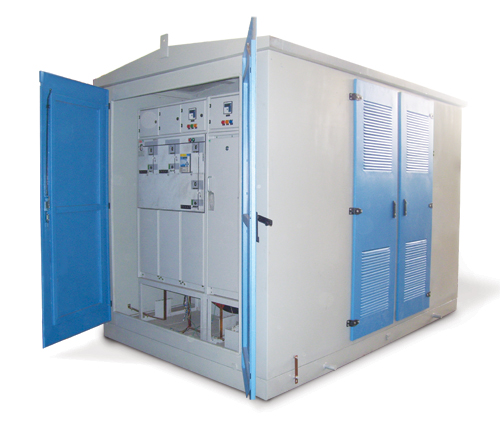
\includegraphics[scale=0.5]{Bilder/Introduction/general_substation.jpg}
\caption{Compact substation with open front panel \cite{bib:comSub}.} \label{fig:compact substation}
\end{figure}

Up until now, SF$_6$ and vacuum-based technology have been dominating the compact medium-voltage switchgear market. Air-insulated switchgear does exist but they are space-consuming and are not applicable for use in a compact substation design. A compact substation is one of the most common designs for substations in the medium-voltage level of the distribution system. Figure \ref{fig:compact substation} displays a compact substation which can be used in the medium-voltage distribution system. The switchgear is a module that can be detached from the substation and removed through its front panel, and can be seen in figure \ref{fig:compact substation}. As figure \ref{fig:compact substation} indicates, there is a limited amount of space available for the switchgear. Therefore, the main challenge for an air-insulated switchgear design for this kind of application is set by the amount of space available in the compact substation.

During current interruption, an electrical arc rises between the contacts the moment they separate. The current will be successfully interrupted if the arc is sufficiently cooled before the current reaches its zero crossing. The amount of cooling needed is based on what type of interruption medium is being used and how large the current in the arc is. SF$_6$-based switchgear designs tends to work without putting too much effort into the cooling design. This is due to the superior interruption capabilities of SF$_6$. When using air, it is more important to evaluate the different parameters that effects cooling: these are mainly pressure and volume flow and can be manipulated via changing of the dimensions in the contact and nozzle geometries.

Due to the efficiency of SF$_6$, little research has been done with optimising of load break switches, since they tend to work easily. To be able to develop air based compact switchgear strong demands are put on optimisation to avoid usage of unnecessary space. Accordingly a test switch have been developed which allows adjustment of design parameter such as nozzle and contact geometry, contact movement speed and material, and upstream gas pressure. For this paper, two different geometries have been developed which will have the same air velocity but a different volume flow. To test the interruption abilities two different current amplitudes will be investigated and the geometries will be compared to each other, and previously tested geometries. The geometries developed for this experiment will be compared to previous similar experiments. These experiments had a higher volume flow than the ones tested here; this gives the opportunity to test if a smaller volume flow can be compensated by an increase in air velocity in the form of increased upstream pressure. Since the air flow velocity and rate are equal when the pin is inside or outside the nozzle it might result in equal interruption capability, no matter the pins position to the nozzle. Previously conducted tests have indicated a poorer interruption rate when the pin is inside the nozzle, partially due to a slower air velocity. It is assumed that the area behind the pin at the moment of interruption also has an impact on the probability of interruption, hence this effect will also be tested. The contact geometries used in this test are quite small compared to previously tested materials and what is common to use in commercially available switches. Therefore, the durability of the contacts will be discussed and compared to the different current magnitudes they are tested on. This might indicate if it is possible to use less material and thereby cut expenses.

This report consists of a Theory section where the typical designs of a load break switch are pointed out, and the working mechanisms of the puffer design concept is also illustrated. Some of the properties of an electrical arc burning in a gas at atmospheric pressure or above is described in the Theory section, while arcs in vacuum behave differently, and will not be featured in this report. The difference between air and SF$_6$ as an interrupting medium is discussed and some of the main challenges when using air are pointed out. Parts of the impact on atmospheric releases of SF$_6$ from load break switches in Norway are also presented in this section of the report.


In the Method section, the contact geometries and materials used in this experiment are illustrated and the air flow through them is discussed. Further in the Method section, the rig and test procedure is explained and followed by the experimental results. The different results are presented; first the success rate for interruption with regards to pressure. This part is followed by the arcing voltage at different upstream pressures, and then the durability of the contacts is displayed mainly in form of pictures. The results are then discussed and the main points from the discussion are presented in the Conclusion part of the report. In the appendix, the raw data from the interruption test is graphically presented, followed by a section about previous relevant research. This section is used to discuss the probability of interruption in the light of the results from previously conducted experiments.

\begin{comment}
TA MED: This report 

A load break switch should be able to interrupt currents less or equal the maximum load current in a distribution system. When interrupting a current the two contacts which a switch consists of start separating producing a gap between each other. Normally the current is not interrupted by this and an electrical arc ignites and burns in the contact gap \cite{bib:HVEbreak}. The arc consists of plasma, which is a mixture of negative and positive ions as well as electrons. Due to the energy dissipation produced by the arc the temperature in the plasma is very high. The electrical conductivity of the plasma channel is dependent of the temperature produced by the arc. When a high current is flowing it is almost a perfect conductor, but at low temperatures the conductivity is much poorer.

An AC-current have a natural zero crossing, as the current approaches this point the arc will start cooling and extinguish if properly cooled at this point of the power cycle. The working principle of a switchgear is to cool the arc sufficiently when the current approaches zero and then quench the arc when the current is zero. At this moment the current is interrupted and a voltage builds up across the open contacts. This voltage is called the recovery voltage. The steepness and amplitude of the recovery voltage \cite{bib:HVEbreak} and the design of the switchgear will decide if a new arc ignites between the contacts after the current zero. If an arc re-ignites ether by a thermal or a dielectric breakdown the interruption has failed. 

Upon till now SF$_6$ and vacuum based technology have been dominating the compact medium-voltage switchgear market. Air insulated switchgear does exists but they are space consuming and are not applicable for use in a compact substation design. A compact substation is one of the most common designs for substations in the medium-voltage level of the distribution system. Figure \ref{fig:compact substation} displays a compact substation which can be used in the medium-voltage distribution system. The switchgear is a module that can be detached from the compact substation and removed trough its front panel. As figure \ref{fig:compact substation} indicates there are a limited amount of space available for the switchgear. Therefore the main challenge for an air insulated switchgear design for this kind of application is set by the amount of space available in the compact substation.

\begin{figure} [h]
\centering
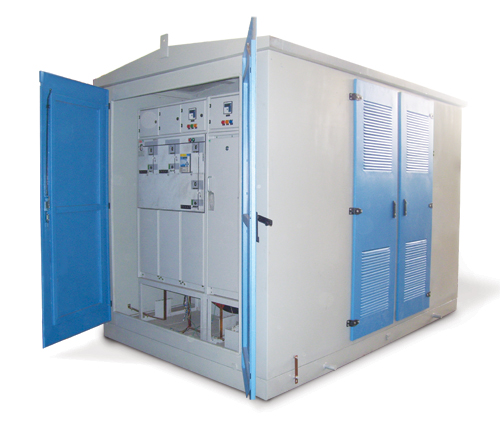
\includegraphics[scale=0.5]{Bilder/Introduction/general_substation.jpg}
\caption{Compact substation with open front panel \cite{bib:comSub}} \label{fig:compact substation}
\end{figure}

The main choice of interrupting media in switchgear has been SF$_6$ since its discovery in the 1970ies. The gas exhibits many properties which is well suited for an isolation gas. It is highly electron negative which gives it good dielectric strength and arc-interrupting capabilities. The breakdown voltage of SF$_6$ is almost three times higher than air at atmospheric pressure \cite{bib:SF6PI}. It has excellent heat transfer properties as an interrupting medium \cite{bib:SF6PI}. The gas also reforms itself when dissociated under the high temperature conditions in an electrical arc. SF$_6$ produces no polymerization, carbon or other conductive deposits during arcing. It is also chemically compatible with most insulation materials and conductive materials \cite{bib:SF6PI}. The gas is also well suited for use in low temperature environments since its boiling point is fairly low even at high pressures. The gas in its stable form is nontoxic, non-flammable and non-explosive. It is also thermally stable and do not decompose at normal operating temperatures for a closed switch \cite{bib:SF6PI}. SF$_6$ based switchgear tends to be cheap to produce relative to other designs, and the gas itself is also affordable at today prices.


SF$_6$ have some disadvantages, when exposed to electrical discharge or arcing it forms highly toxic and corrosive compounds \cite{bib:SF6PI}. It is also hard to remove non-polar contaminants like air and its breakdown voltage is sensitive to water vapour and conductive particles. However it largest downside is probably that it is an effective infrared absorber. This makes it a strong greenhouse gas \cite{bib:SF6PI} and it is regarded to be almost $20000$ times as potent as CO$_2$.

0.4\% of the greenhouse gas emissions in Norway is due to SF$_6$ and is mainly used in switchgear or other high voltage equipment \cite{bib:KlimaKur2020}. In Norway the use of SF$_6$ is regulated through a voluntary contract between the environmental department and the end user, mainly the power companies \cite{bib:KlimaKur2020}. If a compatible air based switchgear design is released on the market it can be assumed that the power companies will be interested in the new technology. It is also possible that the government will restrict the use of SF$_6$ gas if the private sector do not follow the guidelines of the environmental department.

A test switch have been developed which allows adjustment of many design parameter such as nozzle and contact geometry, contact movement and gas pressure. The contacts consist of one female contact, or tulip and one male contact, or pin. The tulip is immovable, while the pin can be opened by a spring trigged by an electromagnet. Previous results have illustrate that most of the successful interruptions have occurred when the pin is outside the nozzle \cite{bib:CIAMVLBS}. Cold air simulations done by Nina Sasaki Aanensen of the different geometries have stated that volumetric flow of air is much lower when the pin is inside the nozzle. The results from previous testing and cold air simulations might suggest that the pin is clogging the nozzle and preventing a good air flow. Therefore a new nozzle geometry has been designed with a doughnut area, the area between the nozzle and the pin, which is bigger than the area of the pin. This is assumed to give a volumetric flow of air that is almost the same when the pin is inside the nozzle as well as outside. The theory has been verified by cold air simulations. However the clogging effect generated by an arc has not been taken into account and it is expected that this will have an impact on the volumetric flow. Two nozzles have been constructed of the new nozzle geometry one with an doughnut area of $44 \ mm^2$ and the other one with an area of $66 \ mm^2$. It is expected that the speed of the air will be constant and the volumetric flow will increase with the doughnut area. This will give an opportunity to test which of these parameters that influence the current interruption capabilities the most.

Several different nozzle geometries are going to be tested and it is assumed that the chance for a successful current interruption inside the nozzle will be approximately the same as outside the nozzle. Since the size of the arc compared to the pin will vary between the different nozzle geometries and current amplitudes, a clogging effect is assumed to occur and might be revealed as an lower interruption success rate for certain geometries.

\end{comment}

\cleardoublepage

\section{Theory}
\subsection{Typical switchgear design and interruption sequence} \label{sec:genDes}
Most of the information in section \ref{sec:genDes} is collected from \textit{"Current Interruption in Power Grids"} by Magne Runde \cite{bib:HVEbreak} \newline

\subsubsection{Switchgear design and operation} \label{sec:InterruptCurrent}
Switchgear can be divided into four main categories:
\begin{itemize}
\item Disconnector Switch
\item Load Break Switch
\item Circuit Breaker
\item Earthing Switch
\end{itemize}

This report will focus on the load break switch (LBS) design. An LBS is designed to be able to interrupt currents with a magnitude that is equal or less than the rated maximum continuous current in a transmission system. An LBS must fulfil the following demands to meet the requirements of the application area:

\begin{itemize}
\item When closed:
	\begin{itemize}
		\item It must act as an perfect conductor.
		\item Be capable of interrupting any load that may arise, without generating too high over-voltages. 
	\end{itemize}
\item When open:
	\begin{itemize}
		\item It must be an perfect isolator.
		\item Be able to close without welding the contacts together, even under short-circuit conditions.
	\end{itemize}
\end{itemize}

A typical operation sequence for a switch is as follows. First a control signal enters the switch and activates the opening mechanisms. The contacts starts to open and a gap forms between them. At the same time, an electrical arc ignites between the contacts, burning in the gap. The gap is filled with some kind of interrupting medium which is usually a gas. For a altering current with a frequency of 50 Hz the current will cross zero 100 times per second, and this crossing is called the current zero (CZ). Direct current interruptions will not be explained in this report. 

At the CZ the arc will extinguish because the current is zero, and a voltage will build up between the contacts.

\begin{equation} \label{eq:U_rec}
u_\mathrm{{recovery}}=u_\mathrm{{supply}}-u_\mathrm{{load}}
\end{equation} 

This voltage is called the recovery voltage and is defined in equation \eqref{eq:U_rec}, where $u_{supply}$ is the voltage on the supply side and $u_{load}$ is the voltage on the load side of the open switch. If the recovery voltage is increasing too fast or has high amplitude, a re-ignition of the arc may occur. There are two different kinds of re-ignition: thermal and dielectric. Thermal re-ignition takes place right after CZ, up to a few microseconds, and is mainly dependent on the recovery voltage's steepness. As the recovery voltage rises and a thermal re-ignition is avoided, a dielectric re-ignition may occur. This kind of re-ignition is largely dependent on the amplitude of the recovery voltage and will occur after a millisecond or more. This paper will mainly focus on thermal re-ignition. If no kind of arc quenching mechanism (like air cooling) is used and the contacts are stationary but open, the arc will re-ignite instantly after CZ, and the normal current sine-wave will be observed. Except in some cases, where the gap is large and the current is small, a successful interruption can occur. The chance for re-ignition will not only be determined by the recovery voltage but will also depend on what kind of interrupting medium is being used. Other factors like contact material, geometry, contact moment speed, and cooling mechanisms are also important to the interruption properties.

Plasma is generated when gas and metal vapour is heated to very high temperatures. At a certain point, the molecules in the gas decomposes to ions and free electrons. This mixture is called plasma, and makes up most of the components in an electrical arc. The physical properties of an arc will be featured in section \ref{sec:eleCondArc} and \ref{sec:HeatTransport}. 

In an LBS, it is important to assure that the switch in closed position acts as a perfect conductor with a low contact resistance. Copper or aluminium are ideal materials and are often used to ensure that this aspect of the switch is met. Sometimes, the contact surface is plated with tin, gold, silver, or platinum to ensure an even lower contact resistance between the contact plates. The main problem with electrical losses in the switch is heat generation, which may speed up metal creeping and other aging-related processes in the switch. Contact plates made of aluminium are especially vulnerable to creeping.
 
To withstand the harsh conditions that occur when an arc burns between the contacts the contact material has to meet strict requirements. It has to tolerate high temperatures and arc erosion, and avoid welding and other stresses that may apply when closing or opening an energized contact. Aluminium and copper are not fit for these tasks since they will melt or erode from the stresses of an arc. It is common to use composites of metals with good electrical conduction with heat-resistant oxides. For high current and voltage switches, it is possible to use a composite of silver or copper together with tungsten or tungsten carbide. These materials are higly heat-resistant, but they also have a high electrical resistance. Therefore, it is common for breakers above $70 \ kV$ to have two sets of contacts: one arcing contact and one main contact. This contact arrangement is  also common at lower voltage levels, and may vary from different designs. The main contact is the first contact to open and the last one to close. This is to ensure that an arc does not start to burn between the main contact, which makes it possible to use aluminium or copper as contact materials. The arcing contact is the last contact to open, and the first one to close, and will ensure that the arc burns between the arcing contact and not between the main contact.

\subsubsection{The puffer principle}
A good circuit breaker design is considered hard to develop and the industry needs to optimise the product to meet the demands set by the market, like size and pressures. This is due to high short-circuit current, in the range of 40 kA and huge recovery voltages. Therefore, the industry has put a lot of effort into circuit breaker development. Nonetheless, when designing an LBS based on SF$_6$, it is common to take the working principle of a circuit breaker and scale it down to a suitable size for an LBS and then test it, and if it works the LBS might be sold on the market without further alterations. When using air, this development technique is not sustainable, since higher demands are set to the switchgear's interrupting capabilities, seeing how the gas is not as efficient as SF$_6$. However, the same interruption techniques will be used but with more weight on optimisation. In the following section, some of these mechanisms will be considered. 

To quench the arc several mechanisms and interrupting mediums can be applied. In today's compact LBS systems based on SF$_6$, the puffer mechanism is commonly used. To obtain a successful interruption of an arc the arc and interruption medium must be cooled down, as well as blow away charged particles and vaporised metal between the contact points. This is the main purpose with the puffer mechanism. 

As SF$_6$ entered the industry in the 1960s, it was in the form of dual pressure breakers. The SF$_6$-based dual pressure breakers had one high pressure chamber, and one low pressure chamber. A valve from a high pressure chamber opened during opening operations, generating a high speed SF$_6$ blast, guided by a nozzle to hit the arc burning between the contacts in the low-pressure chamber. This design has two major disadvantages when using SF$_6$. The switch requires heating to maintain the pressure in the high-pressure chamber to avoid condensation of the SF$_6$ gas. It also uses a compressor to pump the gas from the low-pressure chamber to the high-pressure chamber. This adds to the complexity of the switchgear and may result in more maintenance. The double pressure design was replaced with the newer single pressure design. The single pressure design has only one pressure chamber with low pressure except during interruptions, when the chamber itself becomes a high-pressure chamber.

The single pressure design uses a puffer or the self-blast mechanism to quench the arc, or in some cases a combination of both. The self-blast mechanism is a concept that uses the expansion of the gas to create a pressure difference and a gas flow to cool the arc. Common for both puffer and self-blast mechanisms is that they do not use a compressor to generate the gas flow, but uses the energy stored in the switching mechanisms or generated from the blast itself to interrupt the arc. These mechanisms work the same way for both circuit breakers and load break switches, but will in a load break switch be smaller and less complex. This is because the current amplitudes are smaller and therefore a lower pressure is needed to obtain a successful interruption.

The puffer mechanism is based on a piston to generate a gas flow in the switchgear to extinguish the arc. A typical design of this system consists of using a fixed piston integrated in the contact design. A gas reservoir trapped between the arcing contact and the piston is pushed out as the contact moves apart from each other. Figure \ref{fig:CircutBreakPuff1} displays a typical interruption sequence of breaker based on the puffer design.

\begin{figure} [H]
\centering
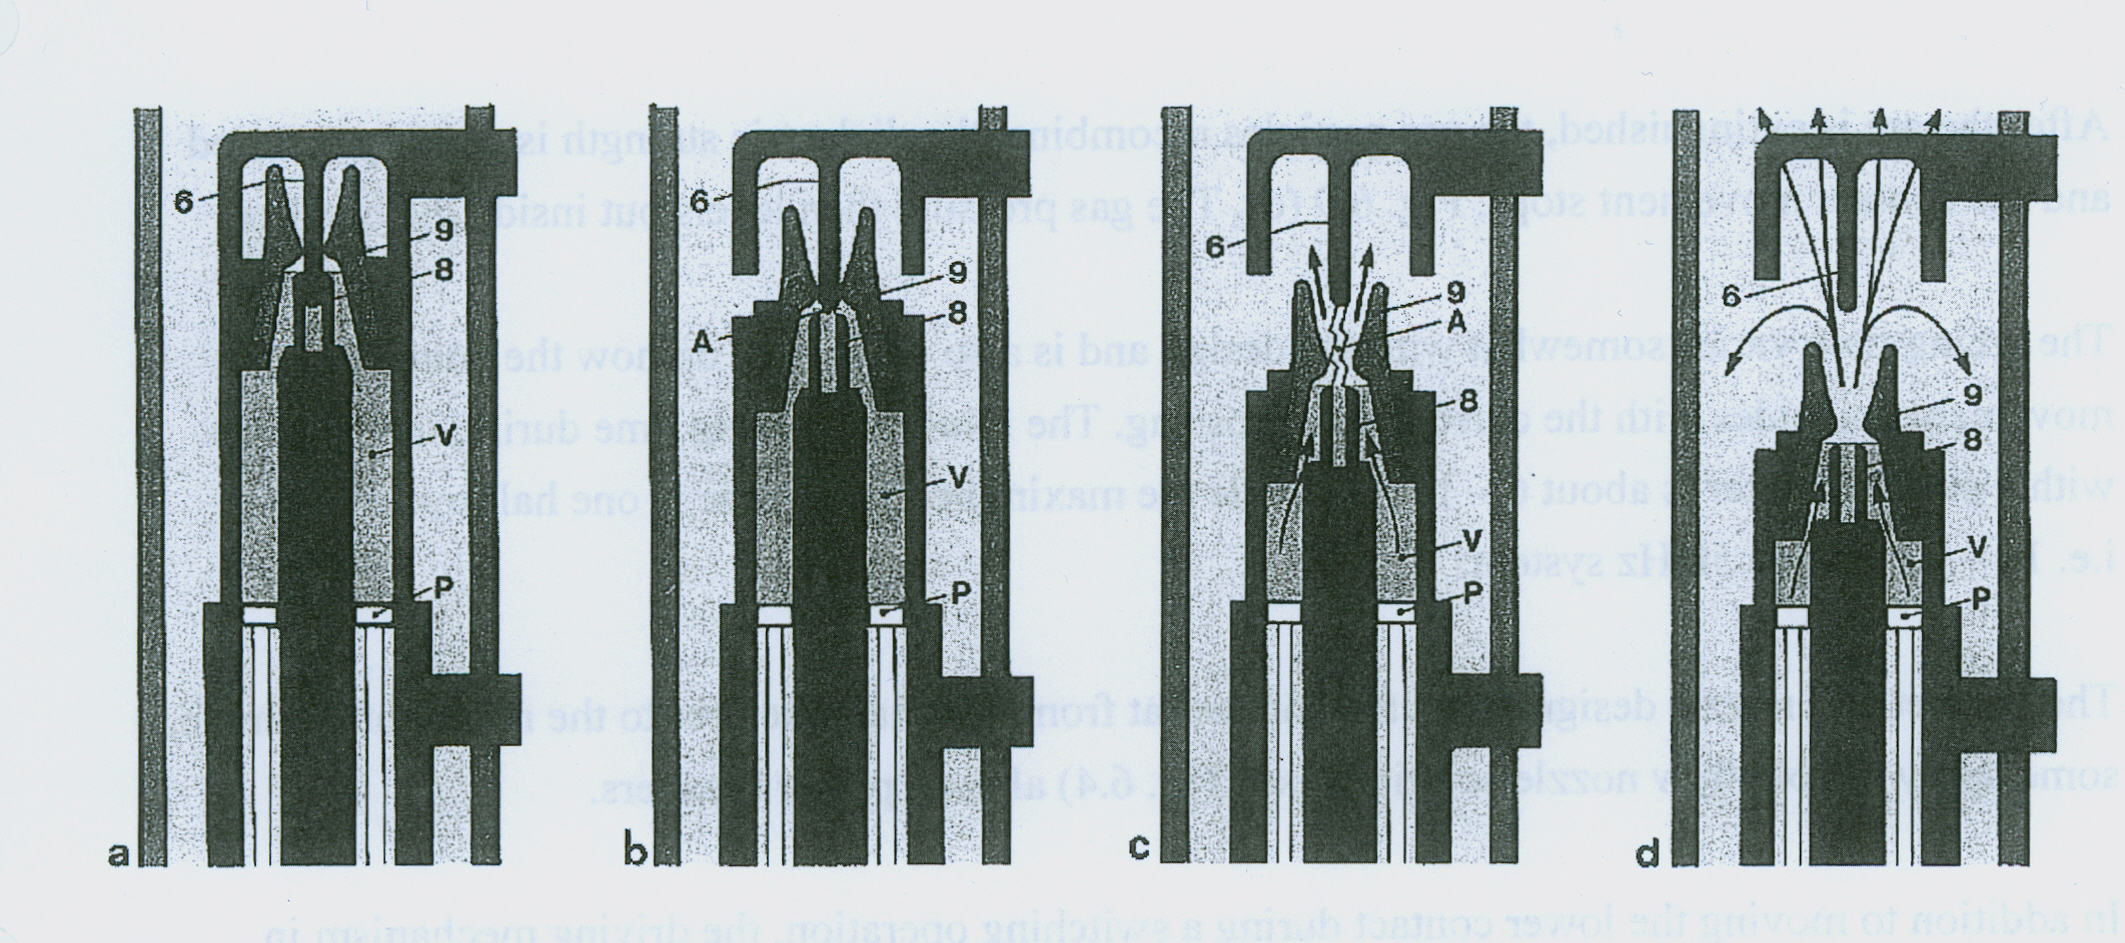
\includegraphics[scale=0.8]{Bilder/Theory/CircutBreakPuff1.png}
\caption{Interruption sequence in a breaker using the puffer mechanism \cite{bib:HVEbreak}.} \label{fig:CircutBreakPuff1}
\end{figure}

When the breaker is closed as seen in figure \ref{fig:CircutBreakPuff1}a, there is a gas volume \textit{(V)} trapped between the piston \textit{(P)} and the arcing contact \textit{(8)} and \textit{(6)}. At the moment the movable part of the arcing contact \textit{(8)} is pulled down, the volume decreases because of the fixed piston, and an increase in pressure due to compression of the gas occurs. Figure \ref{fig:CircutBreakPuff1}b illustrates that the main contact is open and that the current now only flows through the arcing contact.

The next stage of the interruption sequence is pointed out in figure \ref{fig:CircutBreakPuff1}c. The arcing contacts have now separated and an arc \textit{(A)} has ignited between the contacts. The pressurised gas that previously was trapped between the piston and the arcing contact is now released. The gas flow is guided by a nozzle \textit{(9)} that is fixed to the movable arcing contact. The gas flow will cool down the arc and blow away charge carriers between the contact plates. If a sufficient gas flow is obtained, the arc will neither re-ignite after current zero nor extinguish before current zero.

The gas flow is partially dependent on the cross-section of the arc, which again is dependent on the current amplitude. A large current resulting in a large arc may block the hole in the nozzle, preventing a gas flow. This is called current clogging and may occur for certain nozzle designs at high current interruptions. In such an event, the pressure in the gas reservoir will increase further due to compression from mechanical moment of the arcing contact and thermal expansion in the gas because of heating from the arc. When the current amplitude approaches zero, its cross-section will decrease and the clogging effect will end. This will result in a powerful gas blast onto the arc, as indicated in figure \ref{fig:CircutBreakPuff1}d. For smaller current amplitudes, the arc cross-section is smaller and a blocking effect does not occur to the same extent. This generates a less intense gas flow, preventing the current to be interrupted before its natural zero crossing.
 
\begin{figure} [H]
\centering
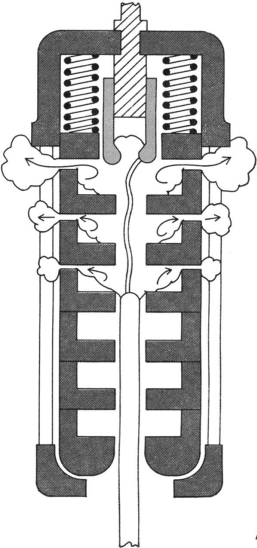
\includegraphics[scale=0.5]{Bilder/Theory/selfBlast.png}
\caption{Expulsion chamber in a breaker using the self-blast mechanism \cite{bib:CBAC}.} \label{fig:selfBlast}
\end{figure}

The self-blast, or third generation breaker, was developed with the goal of reducing mechanical power of the operating system, making it cheaper and less complex. Figure \ref{fig:selfBlast} illustrates the working principle of a breaker using self-blast to interrupt an arc. The difference between self-blast and puffer mechanism is that the puffer mechanism increases the pressure by reducing the volume, rather than the self-blast design which has a constant volume relying on a raise in temperature to increase the gas pressure \cite{bib:CBAC}. The self-blast design uses the heat generated from an arc burning between the arcing contacts to interrupt the current. The gas expands as it is heated by the burning arc. This increase in pressure leads to a gas flow on the arc, which cools it down, leading to the arch being quenched.

There are some disadvantages of the self-blast principle when compared to the puffer mechanism. The self-blast has a lower dielectric strength due to hot gas between the contacts after CZ. This gives a higher chance of re-ignition since hot gas has lower ionisation energy than cold gas. The design is also not well suited to break smaller currents. This is because the arc is less intense and therefore does not heat the gas sufficiently to create a strong enough blast. Therefore, it is common to combine self-blast and puffer mechanism in a hybrid design, so that it can handle both small and large currents. A compact LBS design using air as interrupting medium will probably rely on a puffer design. This is because of the small current an LBS is usually facing compared to a circuit breaker.

%\subsubsection{Test switch}
%A new medium voltage laboratory for load break switch development have been designed with the possibilities to vary important design parameters for a load break switch. When the industry develops switchgear technology they tend to alter several different parameters at the same time. For instance, if they wish to alter the speed of the airflow in a puffer LBS, they might increases the separation speed of the contacts, since these functions often are linked in a puffer design. This will also result in a higher pressure not only and not only a higher volumetric flow. This will make it hard to conclude which parameter that was the most critical for a successful interruption. Therefore a laboratory switch have been design where each of the different parameters can be adjusted without changing other critical parameter. This will make systematic researching possible and optimisation of certain designs criteria, like dimensions, will be a lot simpler.

%\begin{figure} [h]
%\centering
%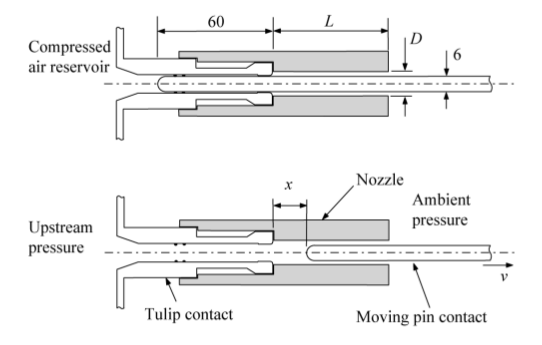
\includegraphics[scale=0.5]{Bilder/Theory/SchematicTestSwitch.png}
%\caption{Test switch} \label{fig:testSwitch}
%\end{figure}

%Figure \ref{fig:testSwitch} shows the physical appearance of the switch and how the different parameter can be adjusted. BLA BLA TAKE A PICTURE OF THE SWITCH, WRITE SOME NUMBERS ON IT. TAKE ABOUT THEM AND WITCH PARAMETERS THAT CAN BE ADJUSTED.

%\begin{figure} [h]
%\centering
%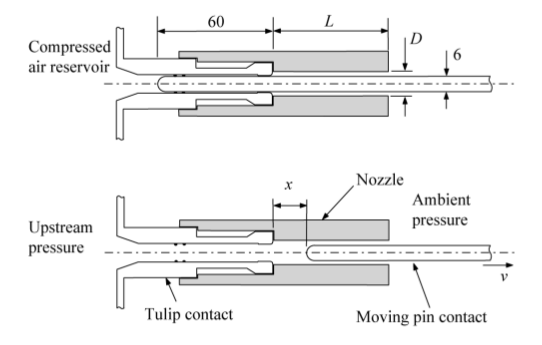
\includegraphics[scale=0.5]{Bilder/Theory/SchematicTestSwitch.png}
%\caption{Tulip, nozzle and pin, L and D is the length and inner diameter of the nozzle, x is contact position. Dimensions are in millimetres.   \cite{bib:CIAMVLBS}} \label{fig:SchematicTestSwitch}
%\end{figure}

%Figure \ref{fig:SchematicTestSwitch} display the former nozzle geometries and it can be clearly seen from this picture that the doughnut area is smaller than the tulip area. It is possible that this will give a clogging effect when the pin is inside the nozzle and result in a poorer airflow and interrupting capabilities for this situation. In figure \ref{fig:differentGeometries} the different contact geometries that have been made is shown. Geometries a1, b1, and c1 have been tested and the results showed that most of the successful interruptions happen when the pin was outside the nozzle. It is possible that this is the result of a clogging effect that takes place between the nozzle and pin. Therefore geometries b2 and c2 was created. The geometries is similar to b1 and c1 since they have the same nozzle area, respectively $44 \ mm^2$ and $66 \ mm^2$. The volumetric airflow will however be smaller for b2 and c2 because it have been created a choking point in the tulip. 

%\begin{figure} [h]
%\centering
%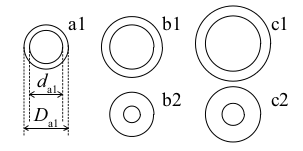
\includegraphics[scale=0.6]{Bilder/Theory/differentGeometries.png}
%\caption{Different contact geometries \cite{bib:CIAMVLBS}} \label{fig:differentGeometries}
%\end{figure}

%It is expected that b2 and c2 will need a higher pressure than b1 and c1 to perform a successful interruption, due to the lower airflow. However it is expected that they will have an equal successrate no matter if the pin is inside the nozzle or outside the nozzle.

\cleardoublepage
\subsection{Interrupting currents} 
%\subsubsection{Phenomenological description of a typical current interruption} \label{sec:InterruptCurrent}
%A interrupting sequence in an AC power system follows a typical pattern. During normal service the contacts are closed and current is flowing through the switchgear without electrical losses. When a command signal to interrupt the current is sent to the breakers driving mechanism the contacts are set to motion. A gap opens between them and is filled with an interrupting medium. An arc usually forms between the contacts and the current continues to flow trough the breaker. This arc mainly consists of plasma which is composed of electrons and other charge carriers like positive and negative ions. Due to energy dissipation in the arc the temperature in the plasma is generally high, but strongly dependent on the amplitude of the electrical current passing through the breaker \cite{bib:HVEbreak}. The system load is the main factor when assessing the electrical current flow through the breaker, the effect from the arcing voltage is often disregarded. Because of the limited time span when assessing breaking operations the sinus curve of the current at a given time is needed to be taken account for. Plasma with an high temperature tends to have a higher electric conductivity than plasma with an lower temperature. Electrical conductivity in an plasma channel is also strongly depend on the medium the plasma is burning in, the difference between air and SF${_6}$ will be discussed in section \ref{sec:airandsf}.

%The arcing voltage, defined as the voltage drop over the arc, is dependent on the temperature and the cross-section of the arc \cite{bib:HVEbreak}, since these are depending on the current the arcing voltage can be regarded as constant when the current exceeds a certain level. This is further explained in section \ref{sec:elarcs} . When the current approaches its zero crossing (CZ) the energy dissipation in the arc decreases and the plasma cools down. With different cooling mechanisms as mention in section \ref{sec:genDes} the breaker cools down the arc. If done sufficient the electric conductivity of the interrupting medium becomes low, and it behaves as an isolator. This will quench the arc as the current amplitude reaches zero.

%The moment after the arc have been quenched a voltage builds up over the contacts, this is called the recovery voltage \cite{bib:HVEbreak}. If a successful interruption is to occur, a re-ignition of the arc must be avoided as the recovery voltage increases. The probability of an re-ignition is set by the steepness and amplitude of the recovery voltage \cite{bib:HVEbreak}. There is two different kinds of re-ignition: thermal and dielectric re-ignition. Thermal re-ignition take place right after CZ and is mainly dependent on the recovery voltage's steepness. As the recovery voltage rises and a thermal re-ignition is avoided a dielectric re-ignition may occur. This kind of re-ignition is largely dependent on the amplitude of the recovery voltage. The recovery voltage can be mathematically expressed as described in equation \eqref{eq:U_rec}. This formula presents a opportunity to analyse the steepness and amplitude of different interrupting scenarios mathematically.

%\begin{equation} \label{eq:U_rec}
%u_{recovery}=u_{left}-u_{right} \cite{bib:HVEbreak}
%\end{equation} 

%Where $u_{left}$ is the voltage on the left hand side of the breaker and $u_{right}$ is the voltage on the right hand side.
\begin{comment}
\subsubsection{Voltage drop in a static electric arc} \label{sec:elarcs}

When working with arcs it is common to differentiate between dynamic and static arcs. The static arc is established during switching operations in a DC power system after the transient phenomenas have faded out. An dynamic arc is an arc that occurs in AC power systems and during the transient part of a DC interruption, or when the cooling of the arc varies with time, like in most puffer designs. Even though all arcs in an AC system is to be regarded as dynamic arcs, it is possible to regard them as static during a short period of time \cite{bib:HVEbreak}.

Figure \ref{fig:staticArcChar} displays the static arc characteristic for an arc burning in a gas filled gap. The figure is only valid for pressure levels equal or above atmospheric pressure. The static arc characteristic gives a relation between the arcing voltage and the electrical current flowing in the gap. The values on the axis is only approximations and varies with the gas type and contact material. The length of the gap is also an important factor the magnitude of the arcing voltage. 

\begin{figure}[H]
\centering
\includegraphics[scale=1]{Bilder/Theory/staticArcChar.png}
\caption{Static arc characteristic  \cite{bib:HVEbreak}.} \label{fig:staticArcChar}
\end{figure}

At low currents the arcing voltage is high, but decreases rapidly with increasing currents. For higher currents the voltage drop is approximately constant, until the current reaches a certain level and the arcing voltage starts to increase. The difference between air and SF$_6$ as an interrupting medium will be discussed further in section \ref{sec:airandsf}, but on a general basis it is likely to assume that SF${_6}$ have a lower arcing voltage if compared to air for a certain breaking operation. This implies that the energy dissipation in air will be higher, especially when breaking smaller currents where the arcing voltage difference is greatest. This is highly relevant for an LBS since most of the switching duties occurs at smaller currents.

An static electrical arc might be regarded as divided into three regions \cite{bib:HVEbreak}.
\begin{description}
\item[Chatode region] The voltage drop, $V_c$, is usually around 20 V.
\item[Arc column]	There is a constant electric field in this region, typical 10 V/cm.
\item[Anode region] The voltage drop, $V_a$, is usually around 3 V.
\end{description}

This relationship is illustrated in figure \ref{fig:potDisArc}.
\begin{figure}[H]
\centering
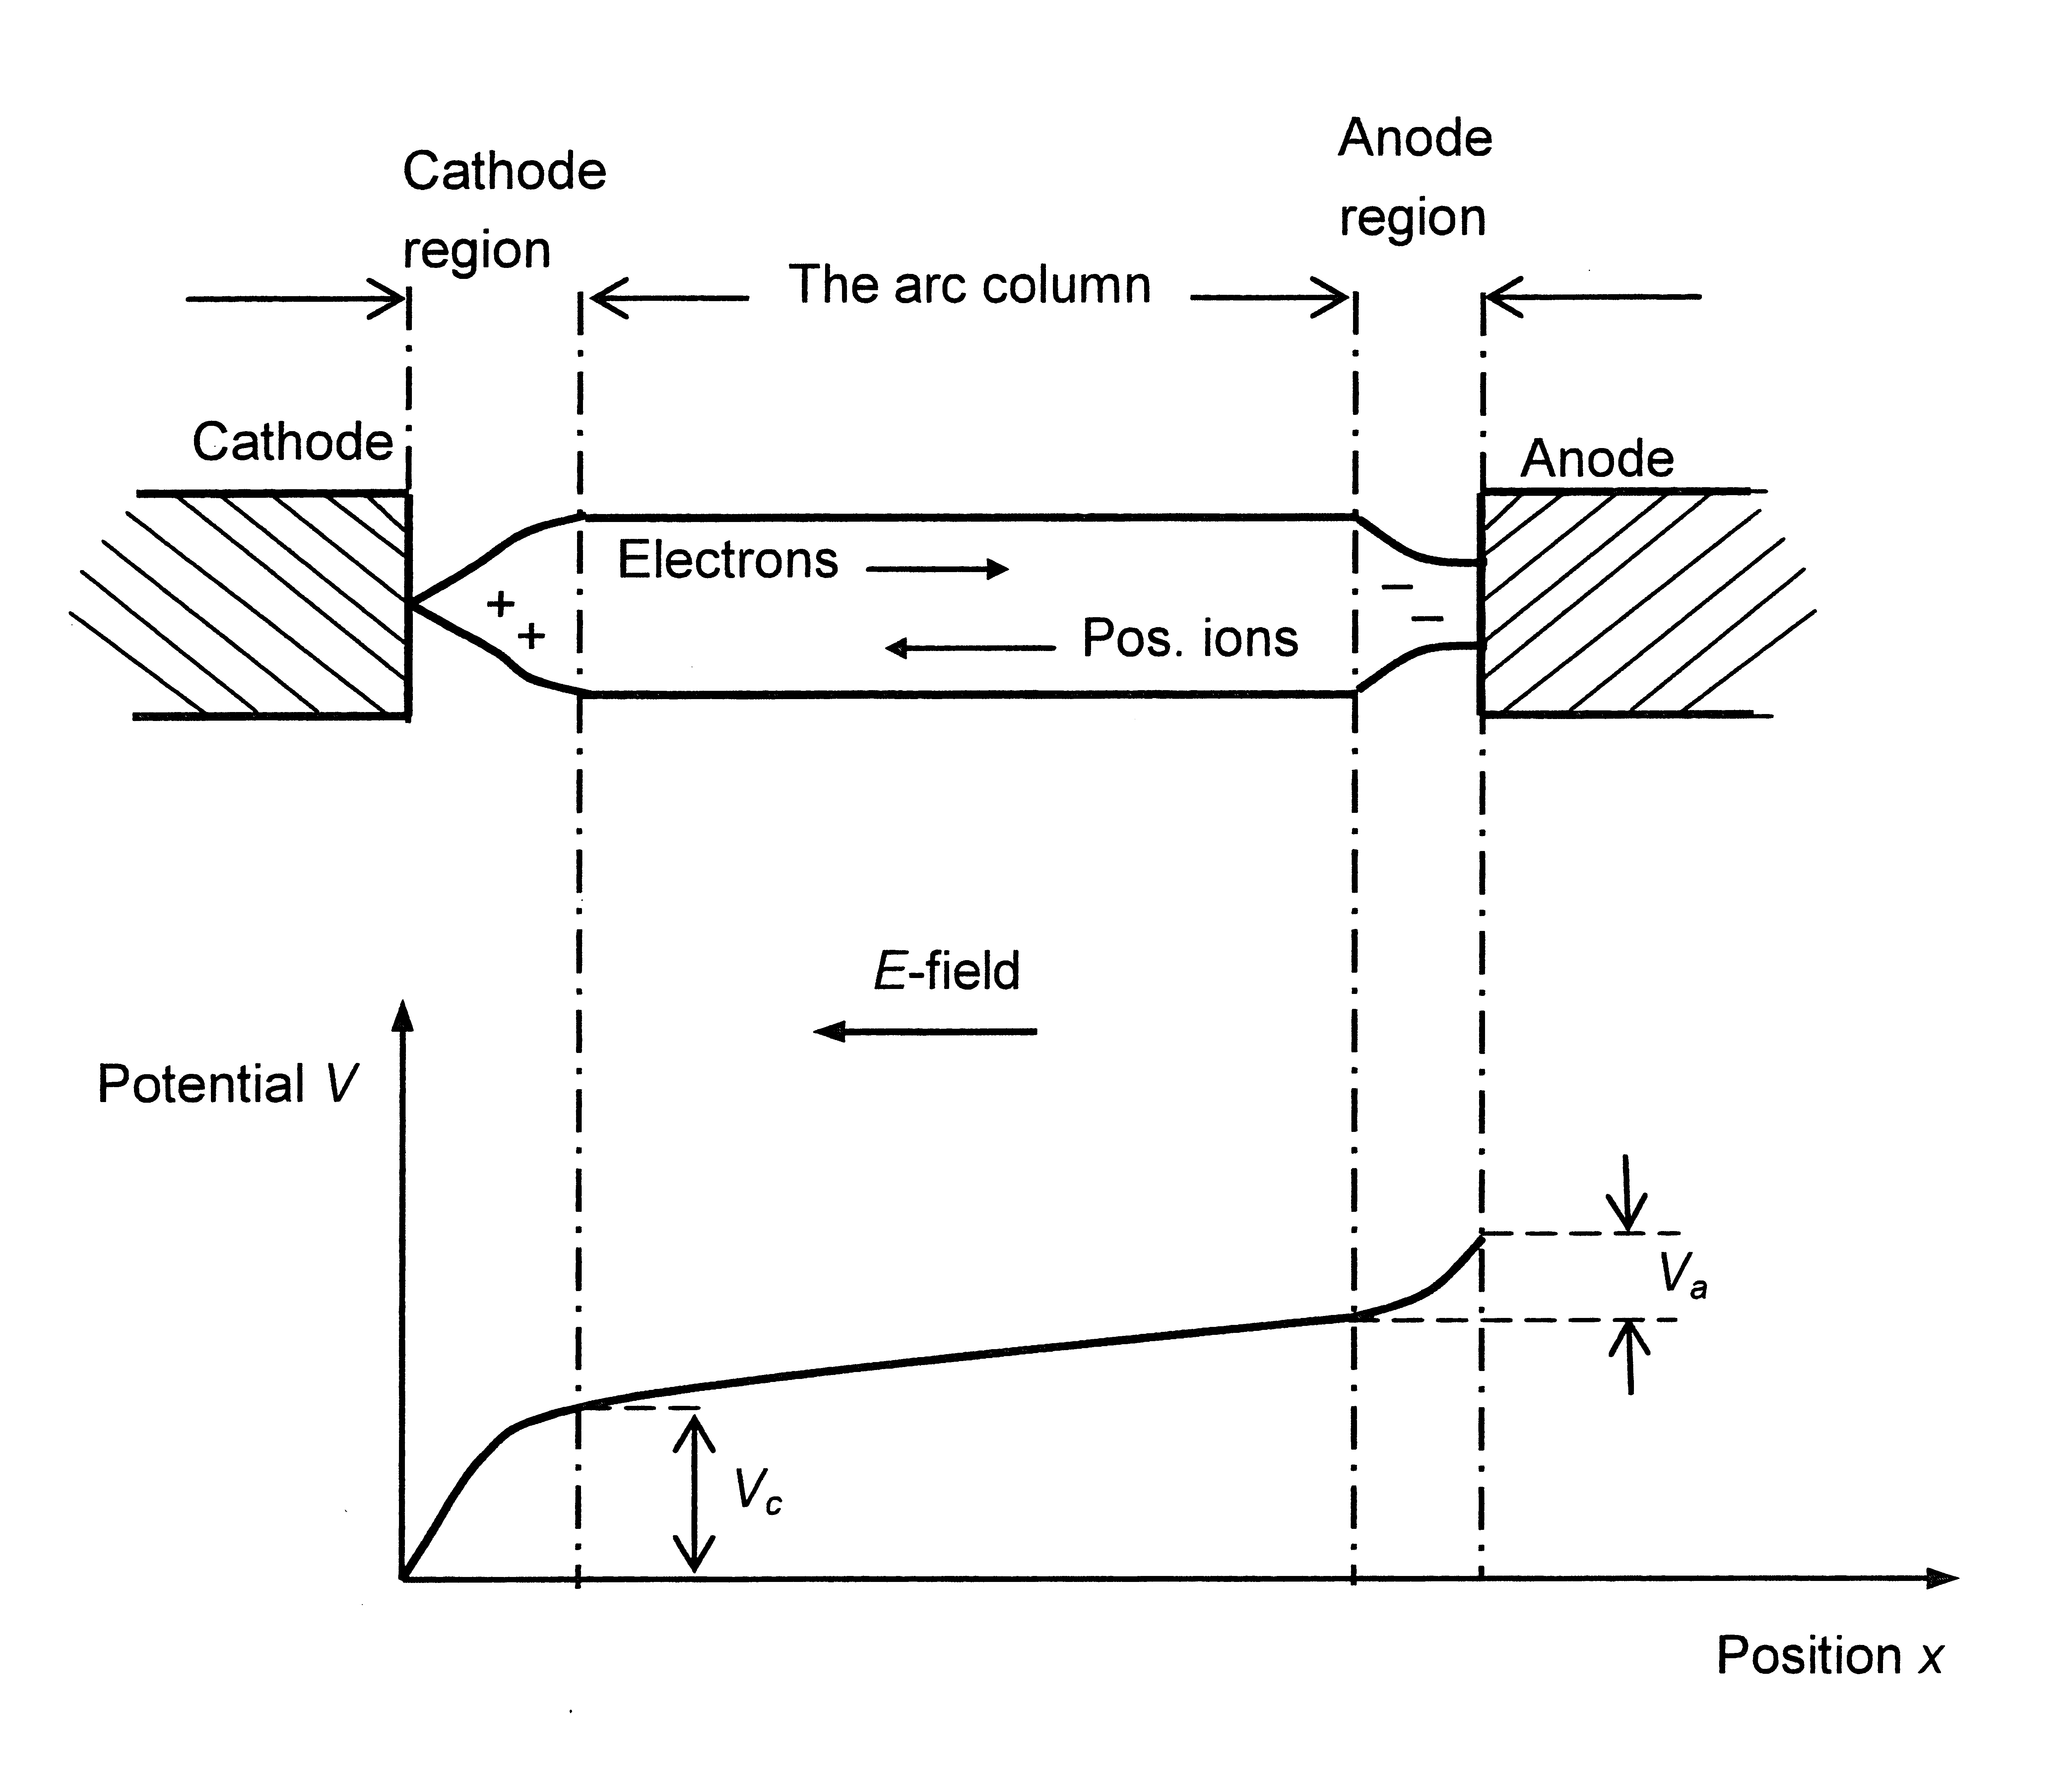
\includegraphics[scale=0.8]{Bilder/Theory/potentialDistArc.png}
\caption{Cross-section of a stationary arc and the corresponding potential distribution \cite{bib:HVEbreak}.} \label{fig:potDisArc}
\end{figure}

For short arcs the voltage drop will mostly occur close to the cathode, and some what at the anode. In longer arcs more of the voltage drop will occur in the arc column itself.
\end{comment}
\subsubsection{Electrical conductivity in an arc} \label{sec:eleCondArc}
Gasses have the ability to be perfect isolators as well as good conductors, mainly depending on the gas temperature. This is due to charged particles and electrons created by dissociation of the molecules in the gas. Air is a mixture of several gasses but might be simplified to consist mostly of nitrogen (N$_2$). In figure \ref{fig:condAir}, the electrical conductivity of air as a function of temperature can be observed.   

\begin{figure}[H]
\centering
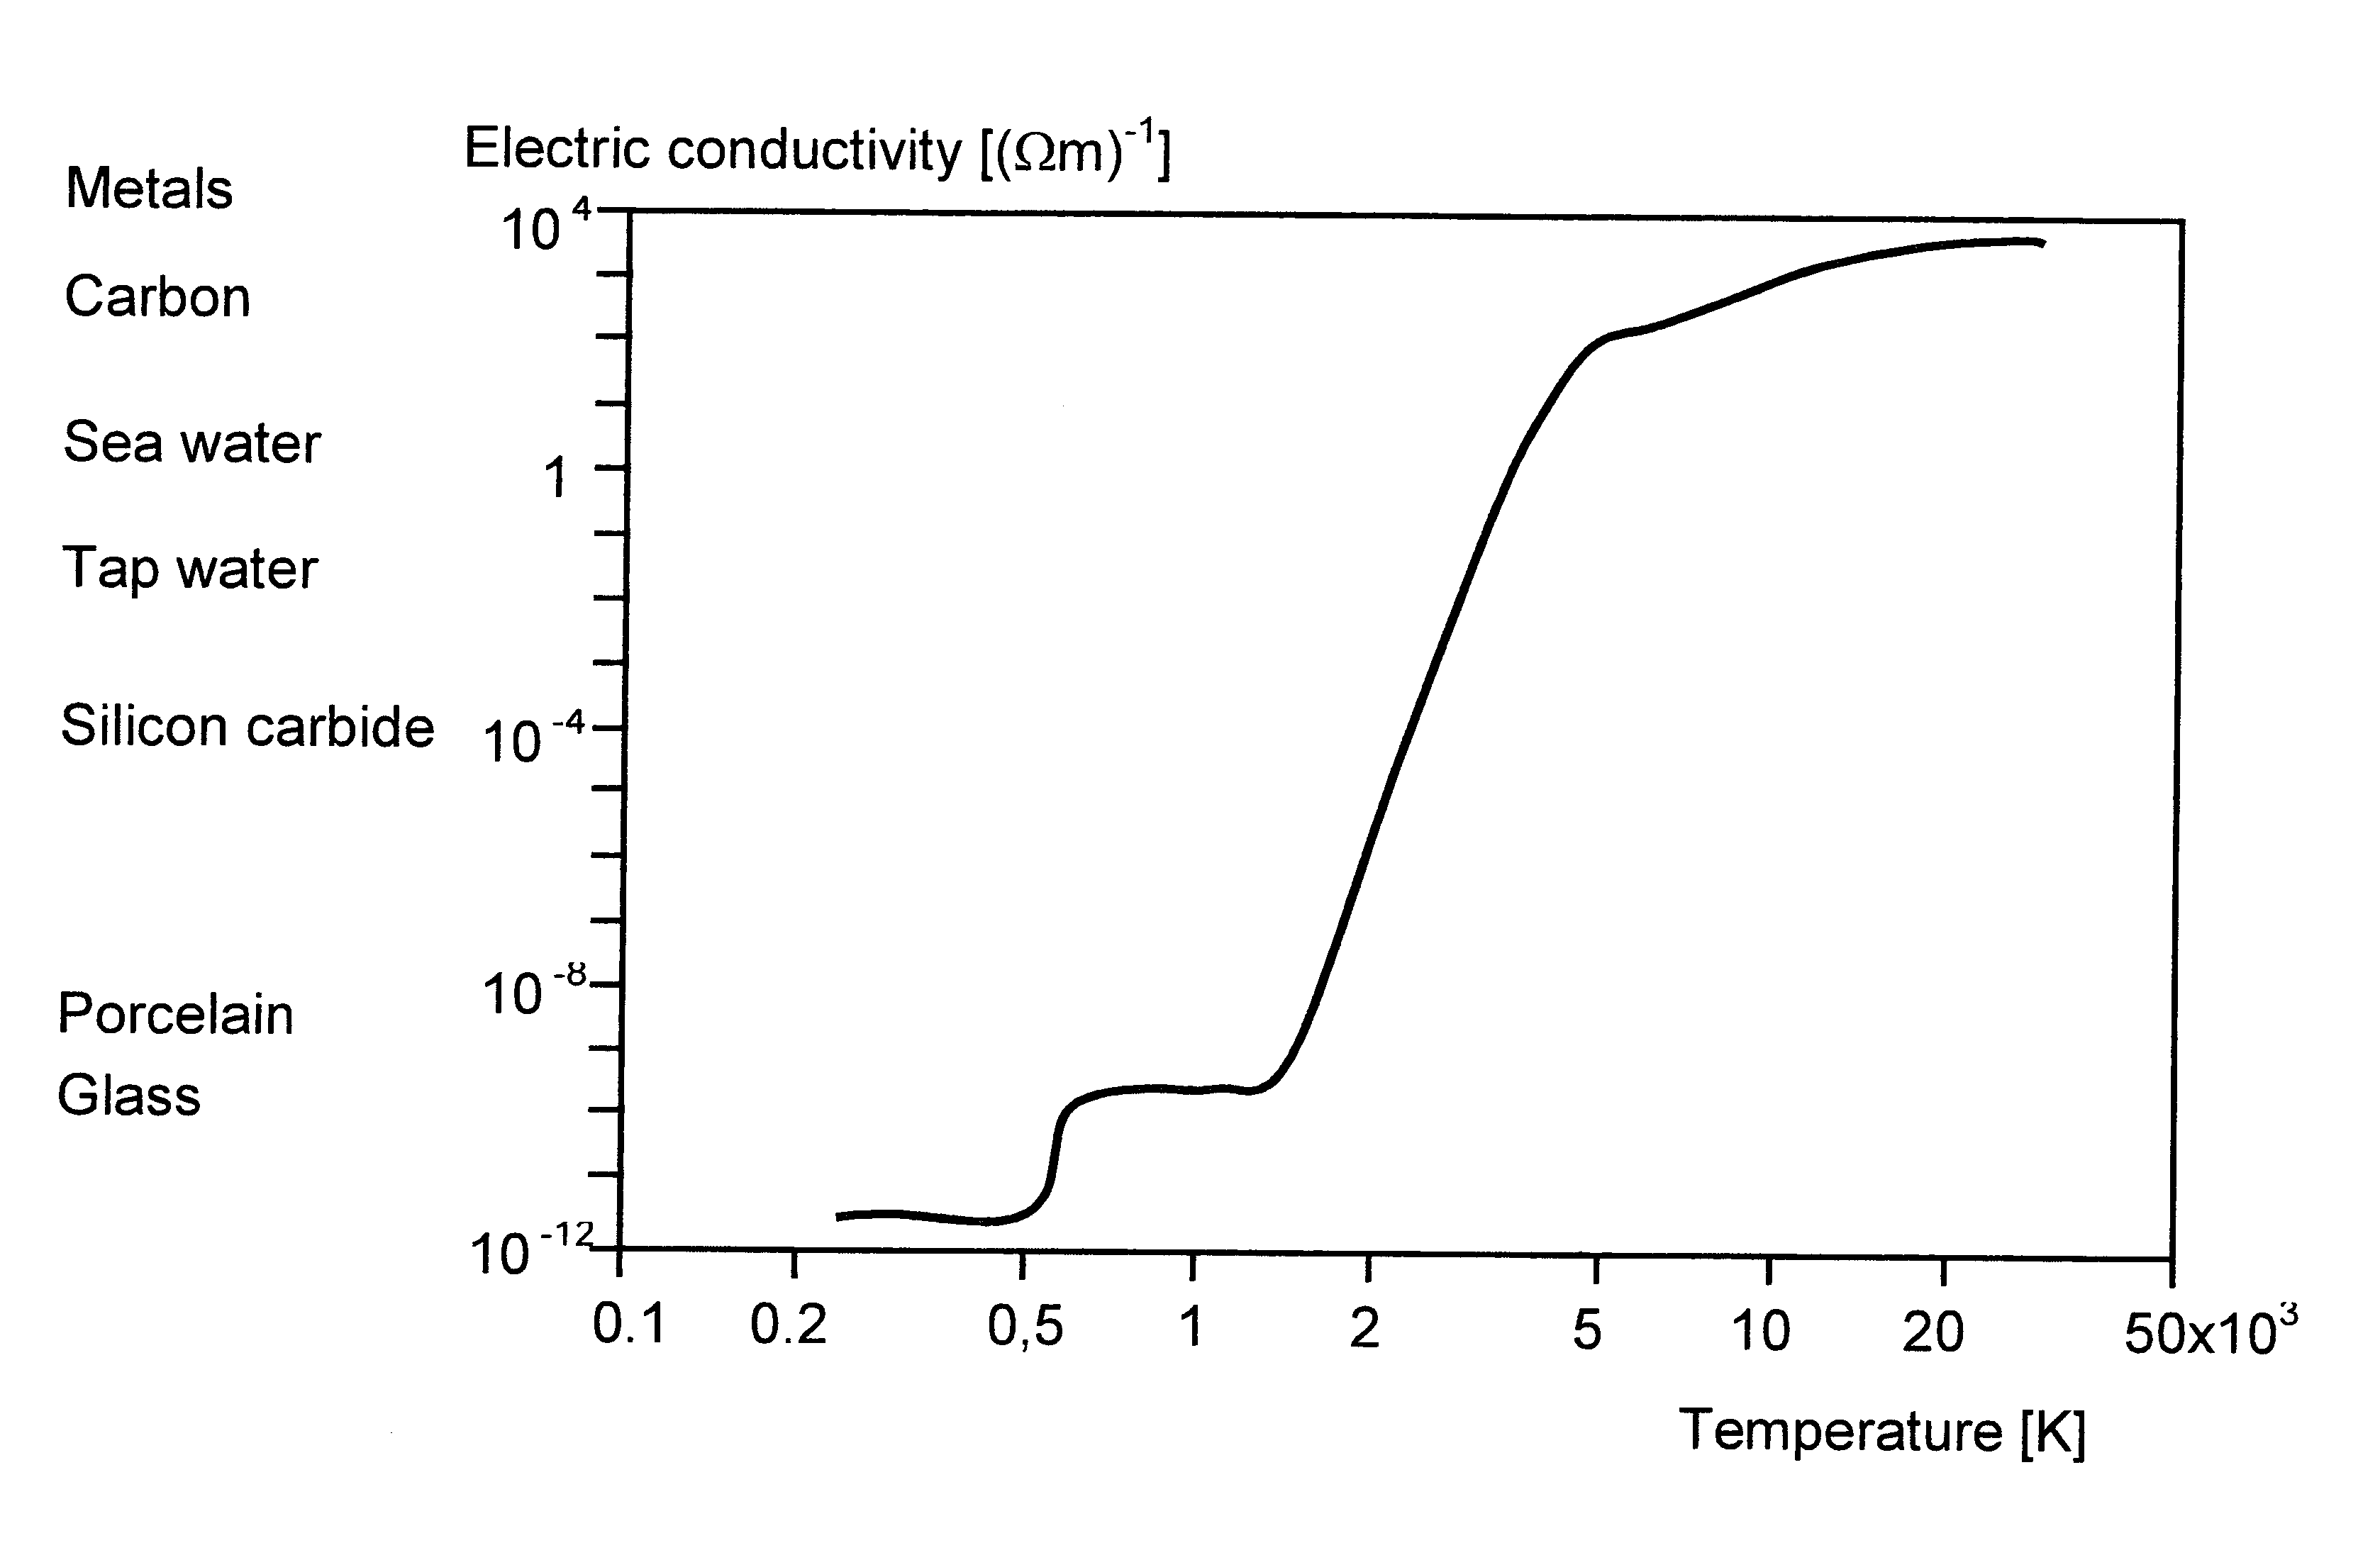
\includegraphics[scale=0.8]{Bilder/Theory/airConduct.png}
\caption{Electrical conductivity of air at atmospheric pressure \cite{bib:HVEbreak}.} \label{fig:condAir}
\end{figure}

The steep increase in conductivity can mainly be explained by the dissociation process and ionization of N$_2$ due to temperature increase. The particle density of nitrogen as it dissociates due to high temperature in the gas is illustrated in figure \ref{fig:Ndensi}. When figure \ref{fig:Ndensi} is compared to figure \ref{fig:condAir}, a connection between temperature and the rapid decline of N$_2$, generation of the positive ion N$^+$, and the steep increase in conductivity of air is clearly presented.

\begin{figure}[H]
\centering
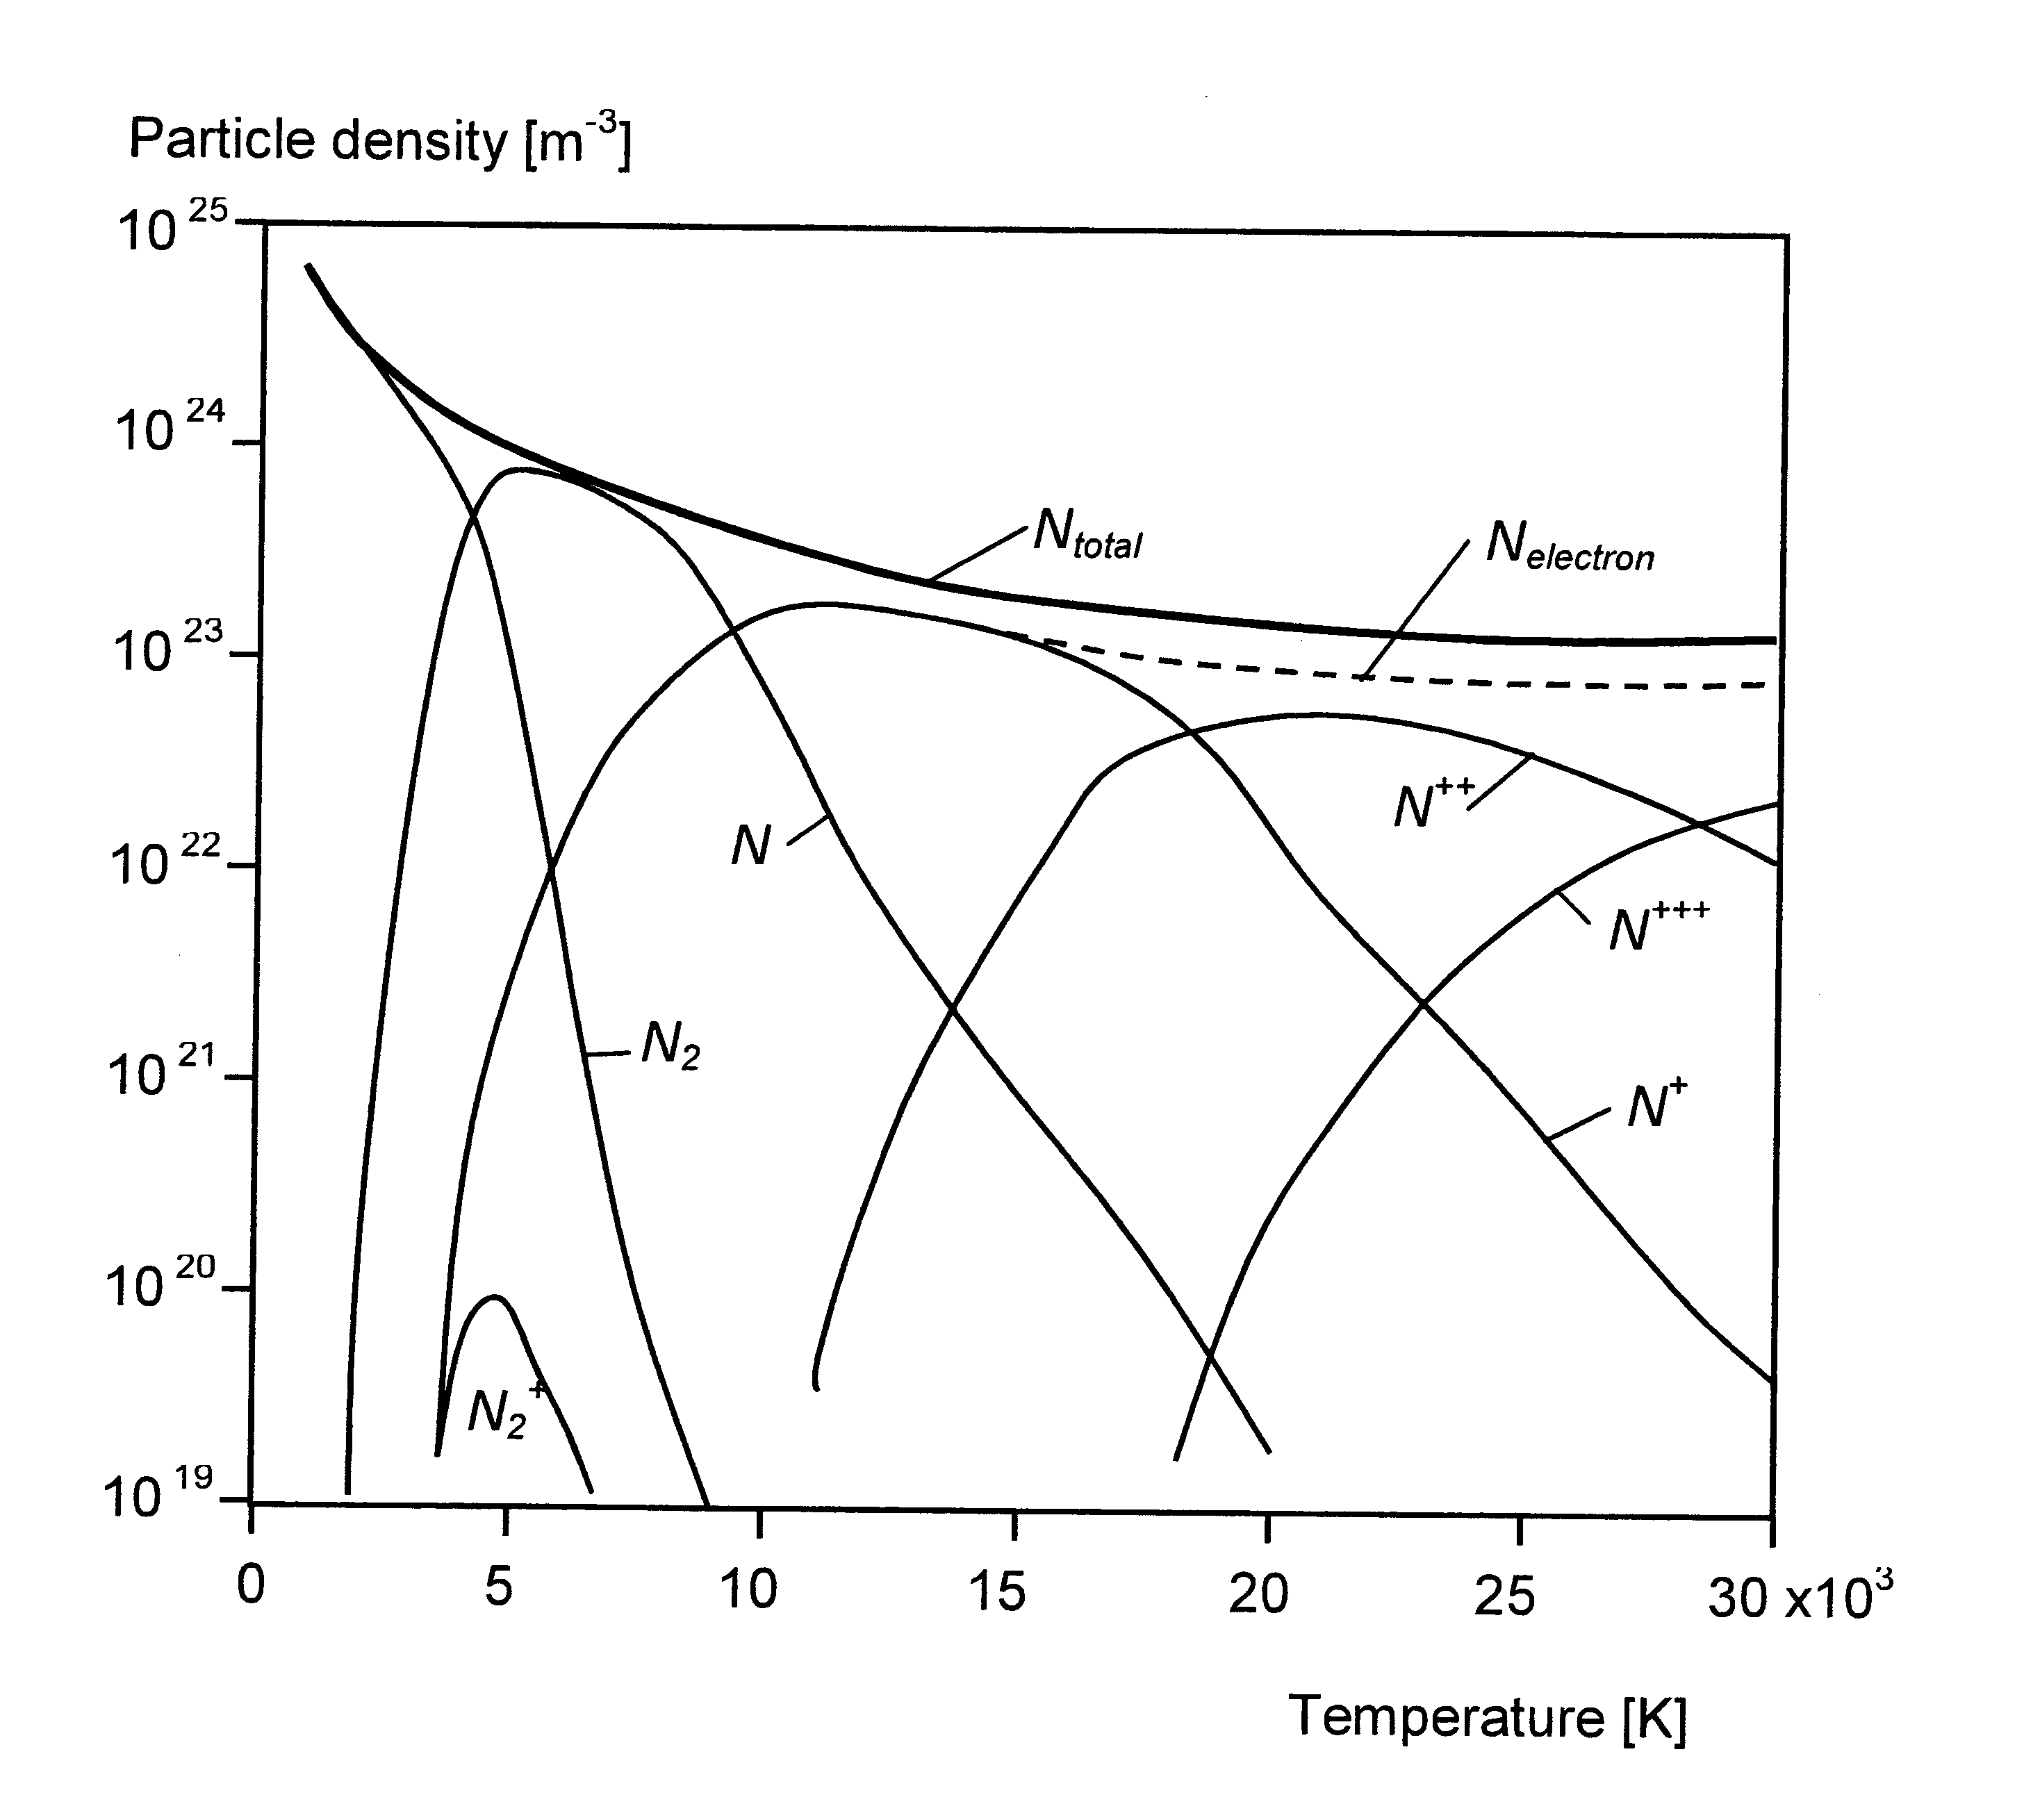
\includegraphics[scale=0.8]{Bilder/Theory/particleDensNit.png}
\caption{Particle density for different dissociation products of nitrogen as a function of temperature \cite{bib:HVEbreak}.} \label{fig:Ndensi}
\end{figure}

From figure \ref{fig:Ndensi}, the electron positive effect of N$_2$ is also indicated via the generation of N$_{2}^{+}$ molecules. From table \ref{tab:thermalIonisation}, the thermal ionisation energy for some gases is presented. This points out that N$_2$ has a significant lower ionisation energy than SF$_6$, and it gives away electrons more easily. However, sulphate and fluorine have a much lower ionisation energy, which is a product of the dissociation of SF$_6$. This indicates that when SF$_6$ first is dissociated, the ionisation and conductivity of the gas rapidly increases. This is also pointed out in figure \ref{fig:SF6densi}, which indicates the particle density of SF$_6$.

\begin{table}[H]
\center
\caption{Thermal ionisation energy for some gases \cite{bib:HVEbreak}.}
\begin{tabular}{|l|c|c|}
\hline 
Particle type & Single ionisation [eV] & Double ionisation [eV] \\ 
\hline 
Air & 16.3 &  \\ 
\hline 
N$_2$ & 15.8 &  \\ 
\hline 
N & 14.5 & 44.1 \\ 
\hline 
O$_2$ & 12.5 &  \\ 
\hline 
SF$_6$ & 19.3 &  \\ 
\hline 
S & 10.4 & 33.8 \\ 
\hline 
F & 17.4 &  \\ 
\hline 
\end{tabular} 
\label{tab:thermalIonisation}
\end{table}

\begin{figure}[H]
\centering
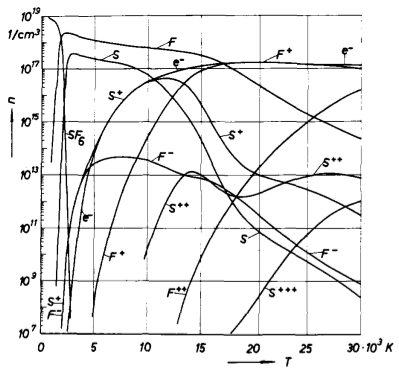
\includegraphics[scale=0.5]{Bilder/Theory/particleDensSF6.png}
\caption{Particle density for different dissociation products of SF$_6$ as a function of temperature \cite{bib:IPSF6AQM}.} \label{fig:SF6densi}
\end{figure}

\begin{figure}[H]
\centering
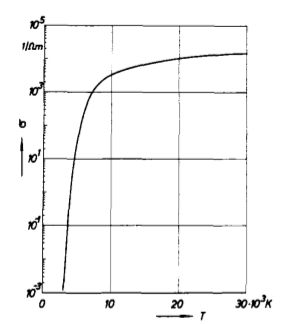
\includegraphics[scale=0.5]{Bilder/Theory/SF6Conduct.png}
\caption{Electrical conductivity of SF$_6$ at atmospheric pressure \cite{bib:IPSF6AQM}.} \label{fig:condSF6}
\end{figure}

In figure \ref{fig:condSF6}, the electrical conductivity of SF$_6$ as a function of temperature is presented. At high temperatures, when SF$_6$ is fully ionised, the conductivity is high, almost in the same range as metals. The transaction between the isolating and the conducting stage is quick.

Decomposed SF$_6$ consists of a high concentration of ionised fluorine, both F$^{+}$ and F$^{++}$. These particles are highly electronegative, which means that they will attract electrons. In air, oxygen has this effect, but the concentration of ionised oxygen is far lower than with fluorine. During a thermal re-ignition, it is the steepness of the recovery voltage that is the most important factor when analysing a thermal re-ignition \cite{bib:HVEbreak}. This is due to the fast acceleration of charge carriers that occurs when the strength of the electrical field between the contacts raises fast, which results in an increase of ionised particles due to collisions. Therefore, removal of electrons is important, since they have a low mass and are set to motion fast.
   
\subsubsection{Heat transportation in an arc} \label{sec:HeatTransport}
There are several different conductive mechanisms in an electrical arc. The effects of these mechanisms vary with temperature, and therefore the heat transport in the arc is strongly dependent upon the temperature. In figure \ref{fig:tempConGas}, several common interrupting gases' thermal heat conductivity is compared to each other as a function of temperature.

\begin{figure}[H]
\centering
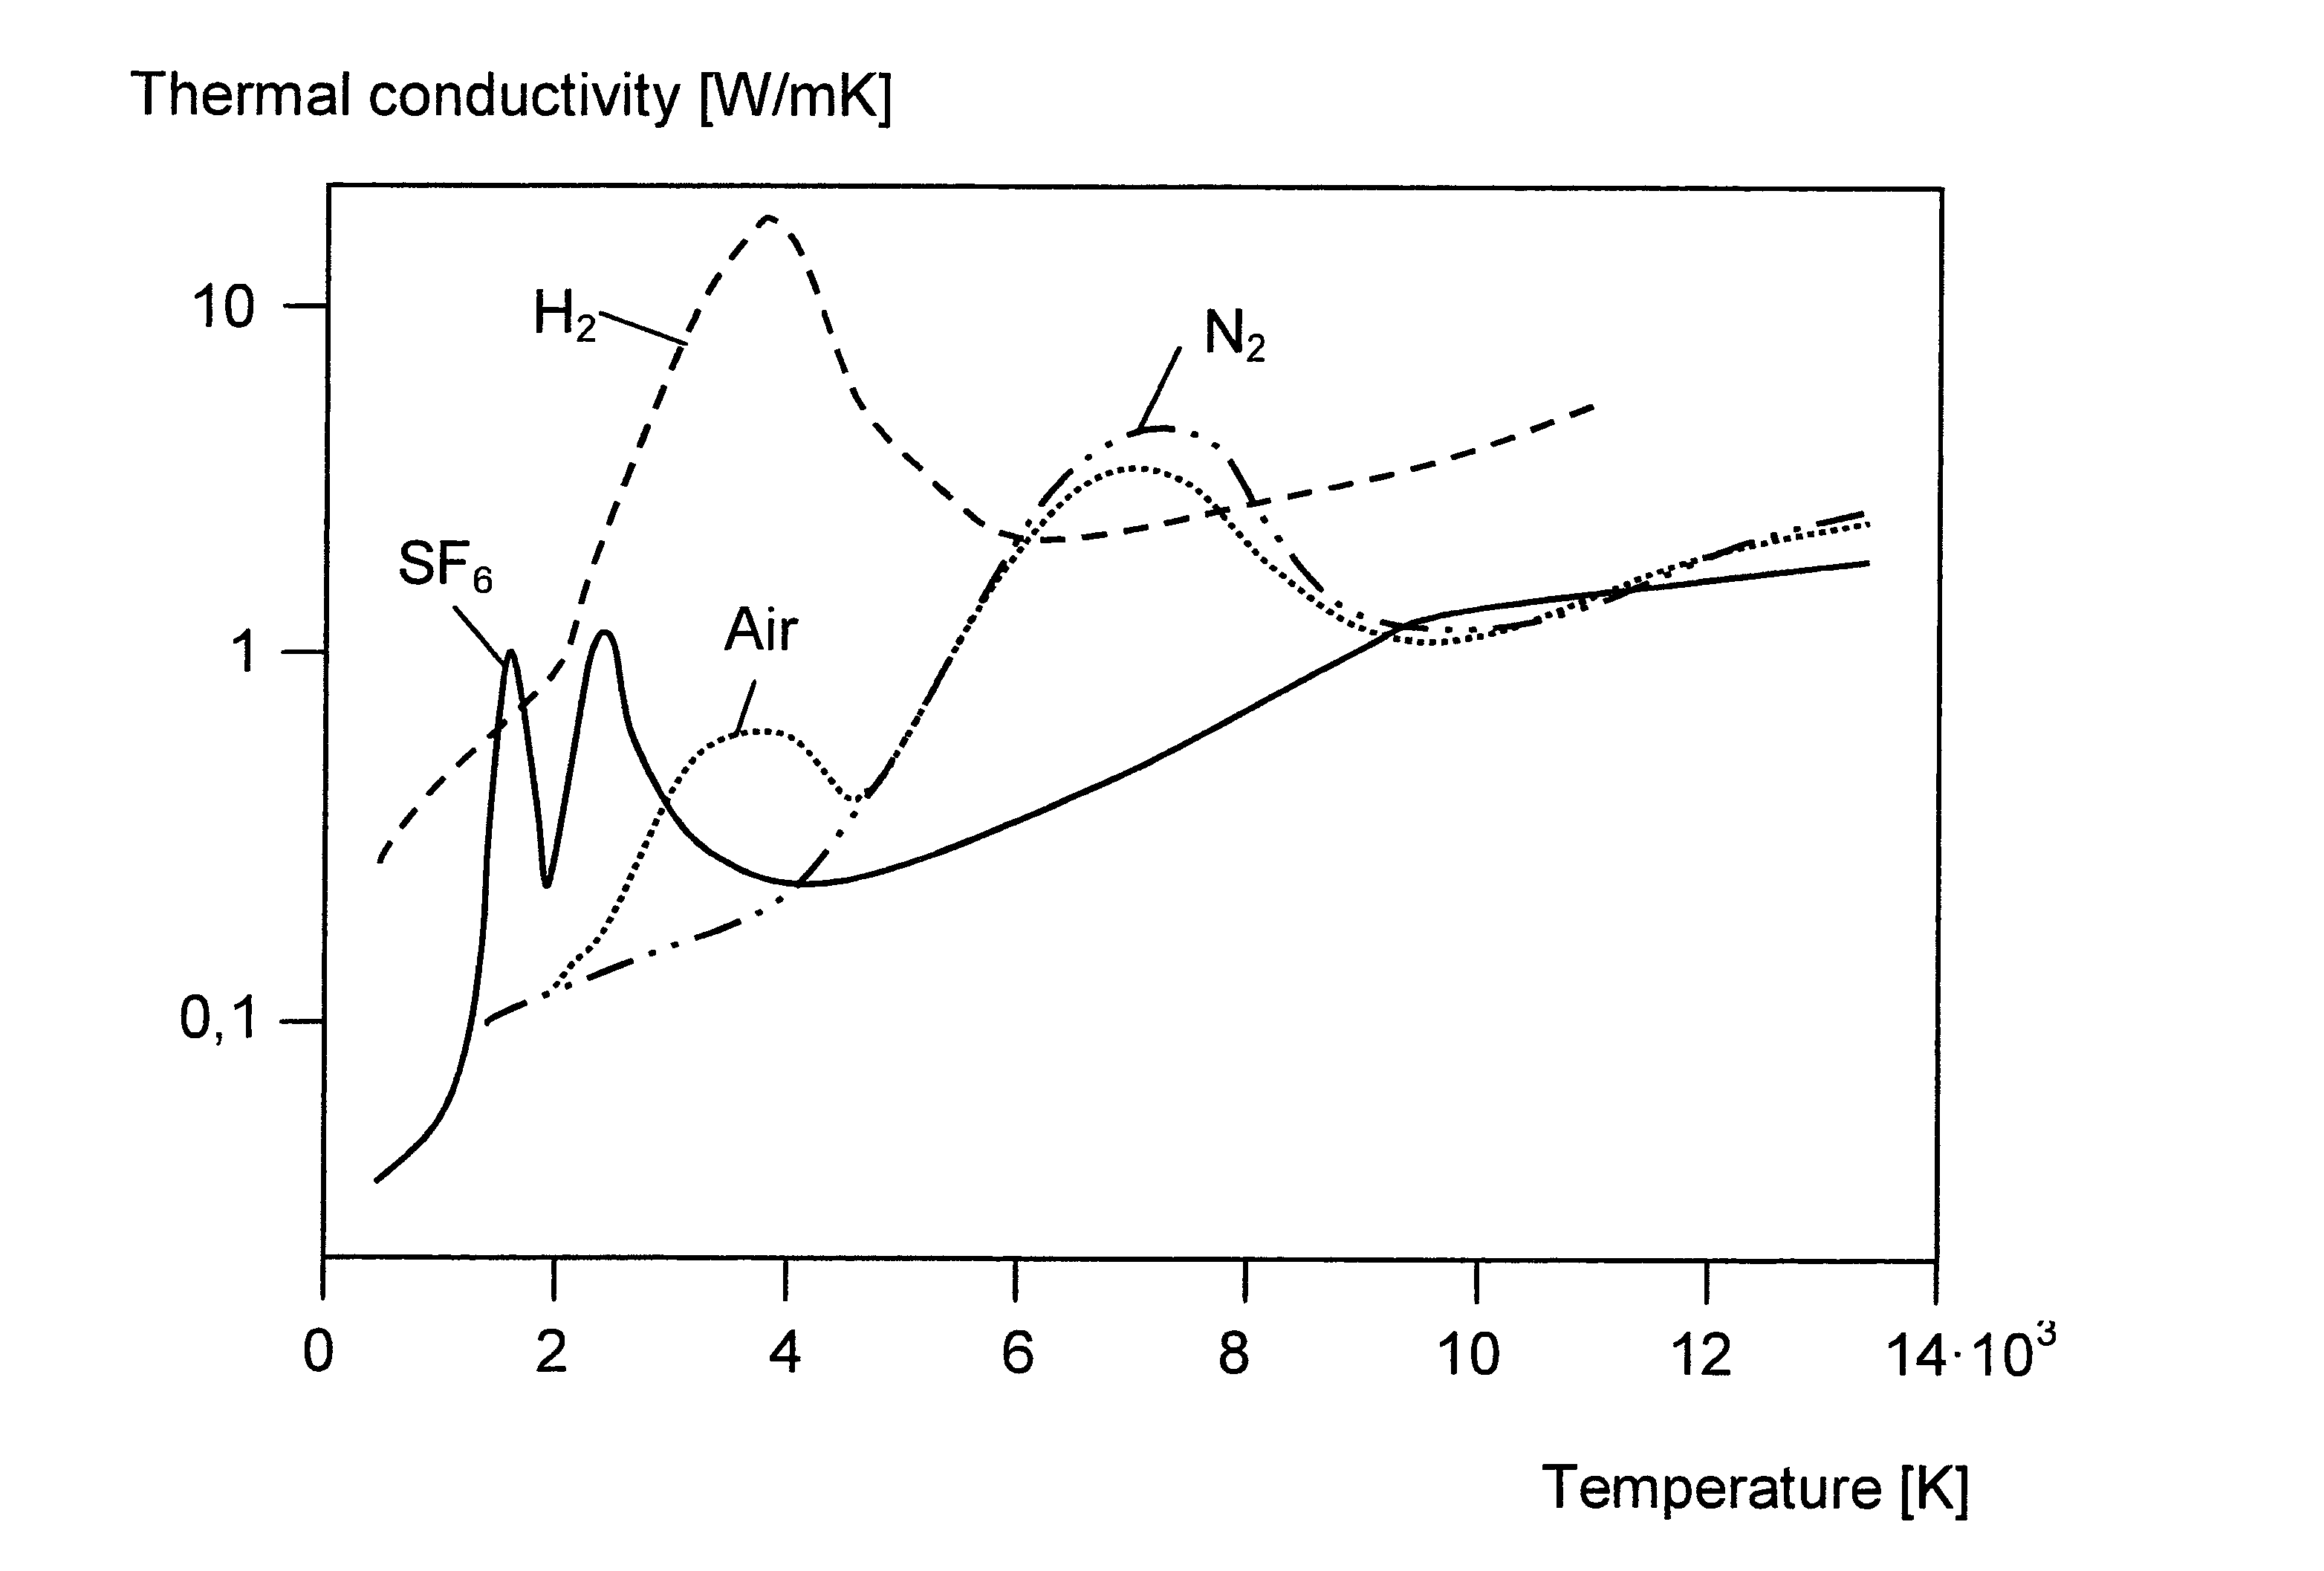
\includegraphics[scale=0.8]{Bilder/Theory/thermalCond.png}
\caption{Thermal conductivity as a function of temperature \cite{bib:HVEbreak}.} \label{fig:tempConGas}
\end{figure}

As illustrated in figure \ref{fig:tempConGas}, the thermal conductivity of air differ quite a lot from the one of SF$_6$. Due to the nature of the different stages in current interruption, it is desired that one uses a gas that has a thermal conductivity that suits the different stages right. 

When the current amplitude is rising, or is high, it is preferred that the thermal conductivity is low. This means that the plasma channel does not heat its surroundings but mainly keeps the dissipated energy stored in its core. This will result in a temperature rise in the plasma channel and a relatively small increase in the surroundings. As explained in section \ref{sec:eleCondArc}, a high arc temperature will result in high conductivity in the arc, which gives a low arcing voltage. If the thermal conductivity is high in this region, heating of the surrounding system will occur. This should be avoided, since it results in unnecessary dissociation of additional interrupting medium. This might result in a slower transaction between the conductive and isolating stage of the interrupting medium, due to the stored energy in the medium and the surroundings, resulting in a higher chance of re-ignition.

At the moment right before CZ, it is an advantage if the thermal conductivity of the gas is high. This will result in a fast cool-down time of the plasma channel since both the current amplitude is decreasing and the energy stored in the arc now is permitted out to its surroundings. A gas with high thermal conductivity in this stage of the interruption process will be able to recombine from an ionised and highly conductive to a non-conductive state fast, making it harder for a thermal re-ignition to occur. This is because of the quick cooling of the plasma channel. In gases where the thermal conductivity is low, the cooling mechanisms are of great importance, since a quick recombination of ionised gas does not occur in the same manner as when the medium is quickly cooled. Therefore, removal of hot gas and charge carriers must be done differently. This is described in detail in section \ref{sec:genDes}.

\begin{figure}[H]
\centering
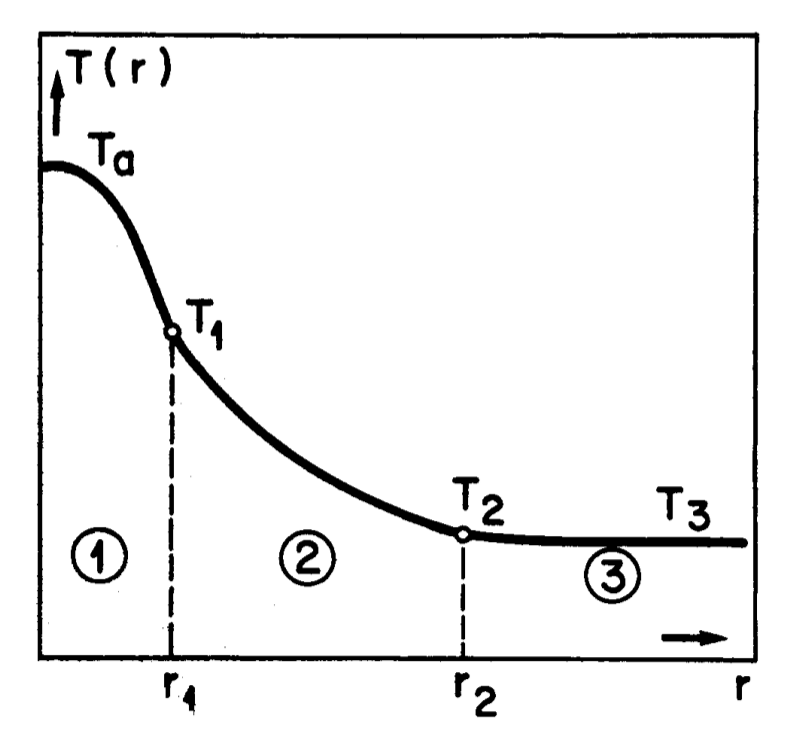
\includegraphics[scale=0.3]{Bilder/Theory/tempZonesArc.png}
\caption{Radial temperature distribution in a plasma channel \cite{bib:TDCIGBB}.} \label{fig:tempDist1}
\end{figure}

The temperature distribution in a plasma channel can be divided into three sections \cite{bib:TDCIGBB}, as illustrated with figure \ref{fig:tempDist1}. Zone 1 is the highly conductive arc core and also the zone with the highest temperature. Zone 2 acts as an energy buffer during the decay of the arc while zone 3 is the cold gas surrounding the arc. When using cooling-mechanisms to quench the arc, it is primarily the second zone of the temperature profile that is cooled. The first zone's temperature will mainly be dependent on the current passing through the arc and will not be influenced by the cooling mechanism in the same degree. If the cooling is sufficient, the energy stored in zone 2 when the arc approaches CZ is low and therefore its effect as an energy buffer is reduced, resulting in a rapid decline in temperature in the arc core as the current approaches zero. This makes the interrupting medium's ability to transport energy important when investigating efficient cooling methods. As figure \ref{fig:tempConGas} has pointed out, SF$_6$ has the ability to transfer heat between zone 1 and 2 fast in the right temperature range compared to the interrupting sequence. Air has to a lesser degree the ability to do this.

\begin{figure}[H]
\centering
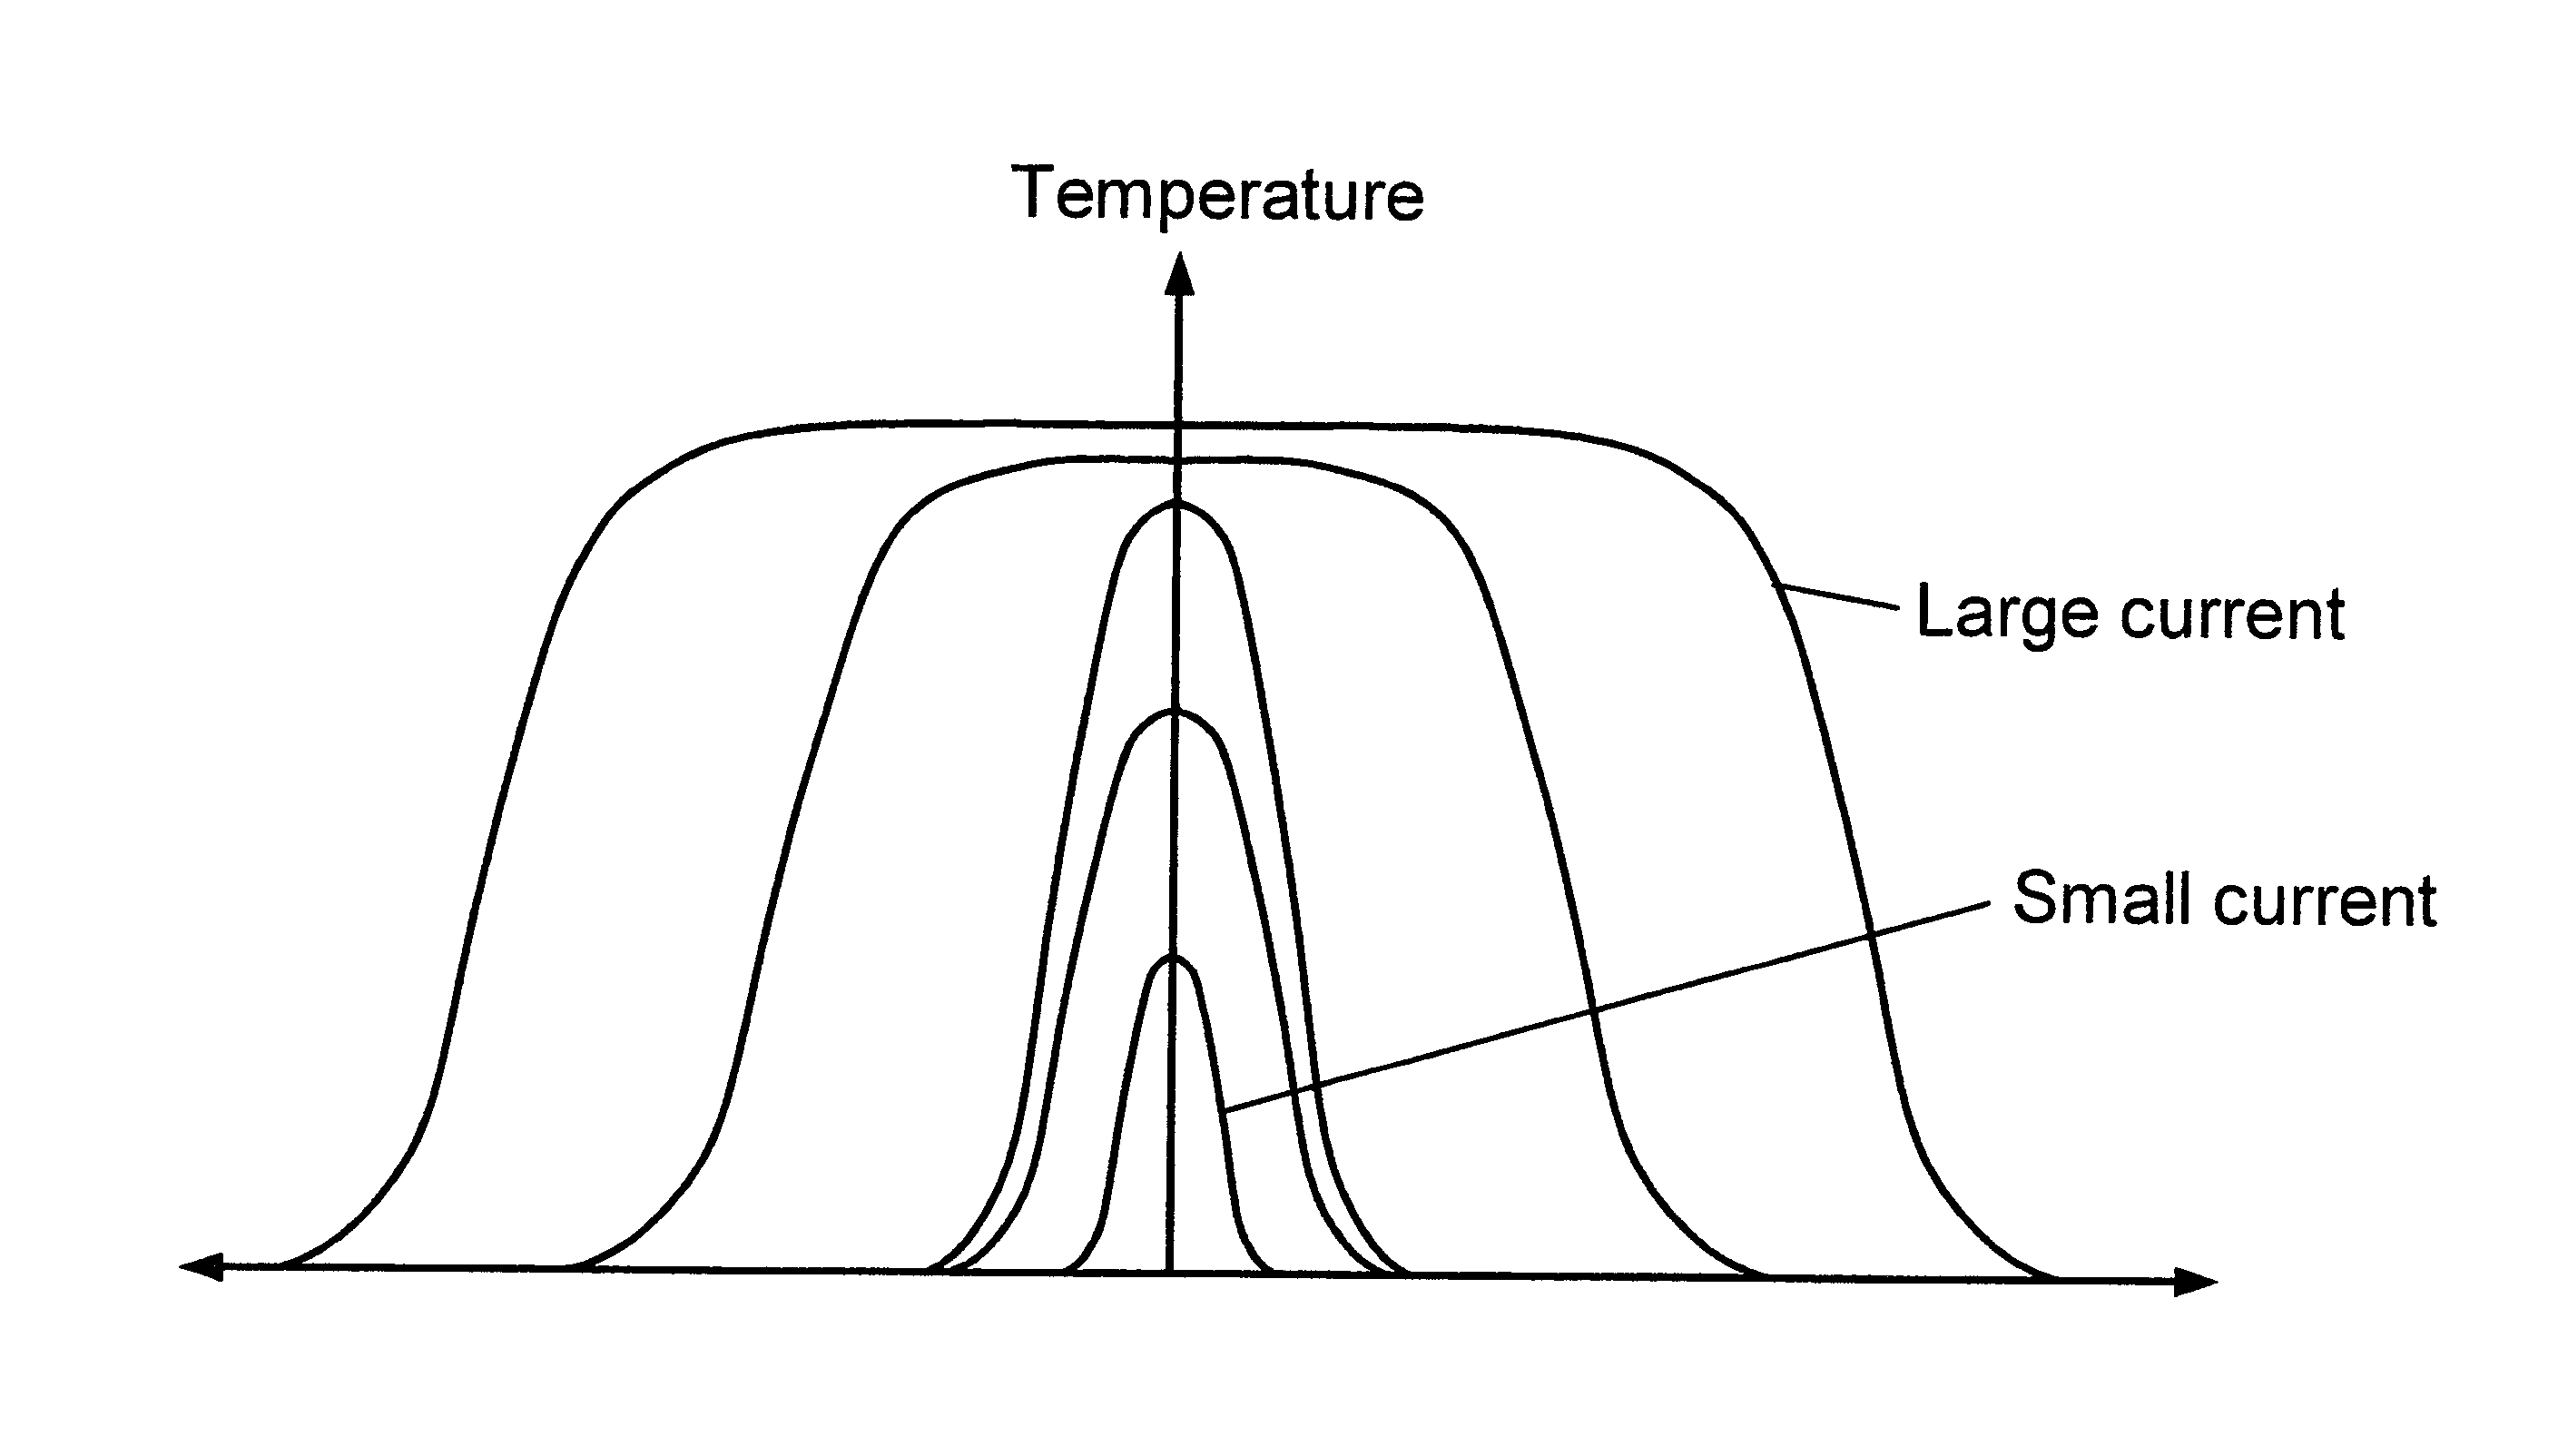
\includegraphics[scale=0.8]{Bilder/Theory/plasmaChannel1.png}
\caption{Radial temperature distribution in a plasma channel \cite{bib:HVEbreak}.} \label{fig:tempDist2}
\end{figure}

In figure \ref{fig:tempDist2}, it is illustrated how the temperature distribution varies with the electrical current. Due to radiation losses in the arc, the temperature has a upper limit of about 20 000 K to 30 000 K. At this point the cross-section of the arc will increase rather than the temperature \cite{bib:HVEbreak}. However, it is not common for an LBS to experience these temperature ranges, and its temperature distribution will mainly be in the lower current part of the figure.

\subsubsection{The difference between air and SF$_6$ as interrupting medium} \label{sec:airandsf}

Although SF$_6$ is superior to air as an interruption medium, air is fairly good, and has been successfully used in the past to interrupt high currents at high voltages, with some air-blast breakers still in use. The primary difference between the two gases when used as interrupting medium is the required dimensions of the switchgear. Traditionally, circuit breakers using air as an interrupting medium and not SF$_6$ have been larger and have used higher pressures to interrupt the current. When producing circuit breakers and larger load break switches, optimization and careful design regarding material, usage, and dimensions must be taken into account. When designing load break switches for medium voltage levels, it is common in some cases to take design principles from circuit breakers and have them scaled down and re-used in load break switches. This gives reason to believe that some of the compact load break switch designs that are on the market today are in fact over-scaled. If they are over-scaled, it might be possible to keep the dimensions equal and exchange the interrupting gas from SF$_6$ to air. However, careful optimisation must be done to meet the demands to dielectric strength and interruption capabilities. Since most of the research on switchgear technology is done on circuit breakers, the difference between air and SF$_6$ on a medium voltage load break switch may not be directly linked with the difference when regarding circuit breakers. Without regards to this, some of the main differences and challenges with the use of air instead of SF$_6$ are pointed out below.

\subsubsection*{Electrical conductivity}
%As expressed in section \ref{sec:eleCondArc} the transaction from isolating stage to a conductive stage for both air and SF$_6$ is quit fast, and the conductive properties are good for both gases. In figure \ref{fig:AirandSF6ConComp} below the conductivity of air and SF${_6}$ is compared. Even though air and SF$_6$ have approximately the same conductivity when dissociated there are some differences in the ionization products of the gases. These differences represent one of the biggest differences regarding electrical conductivity.

\begin{figure}[H]
\centering
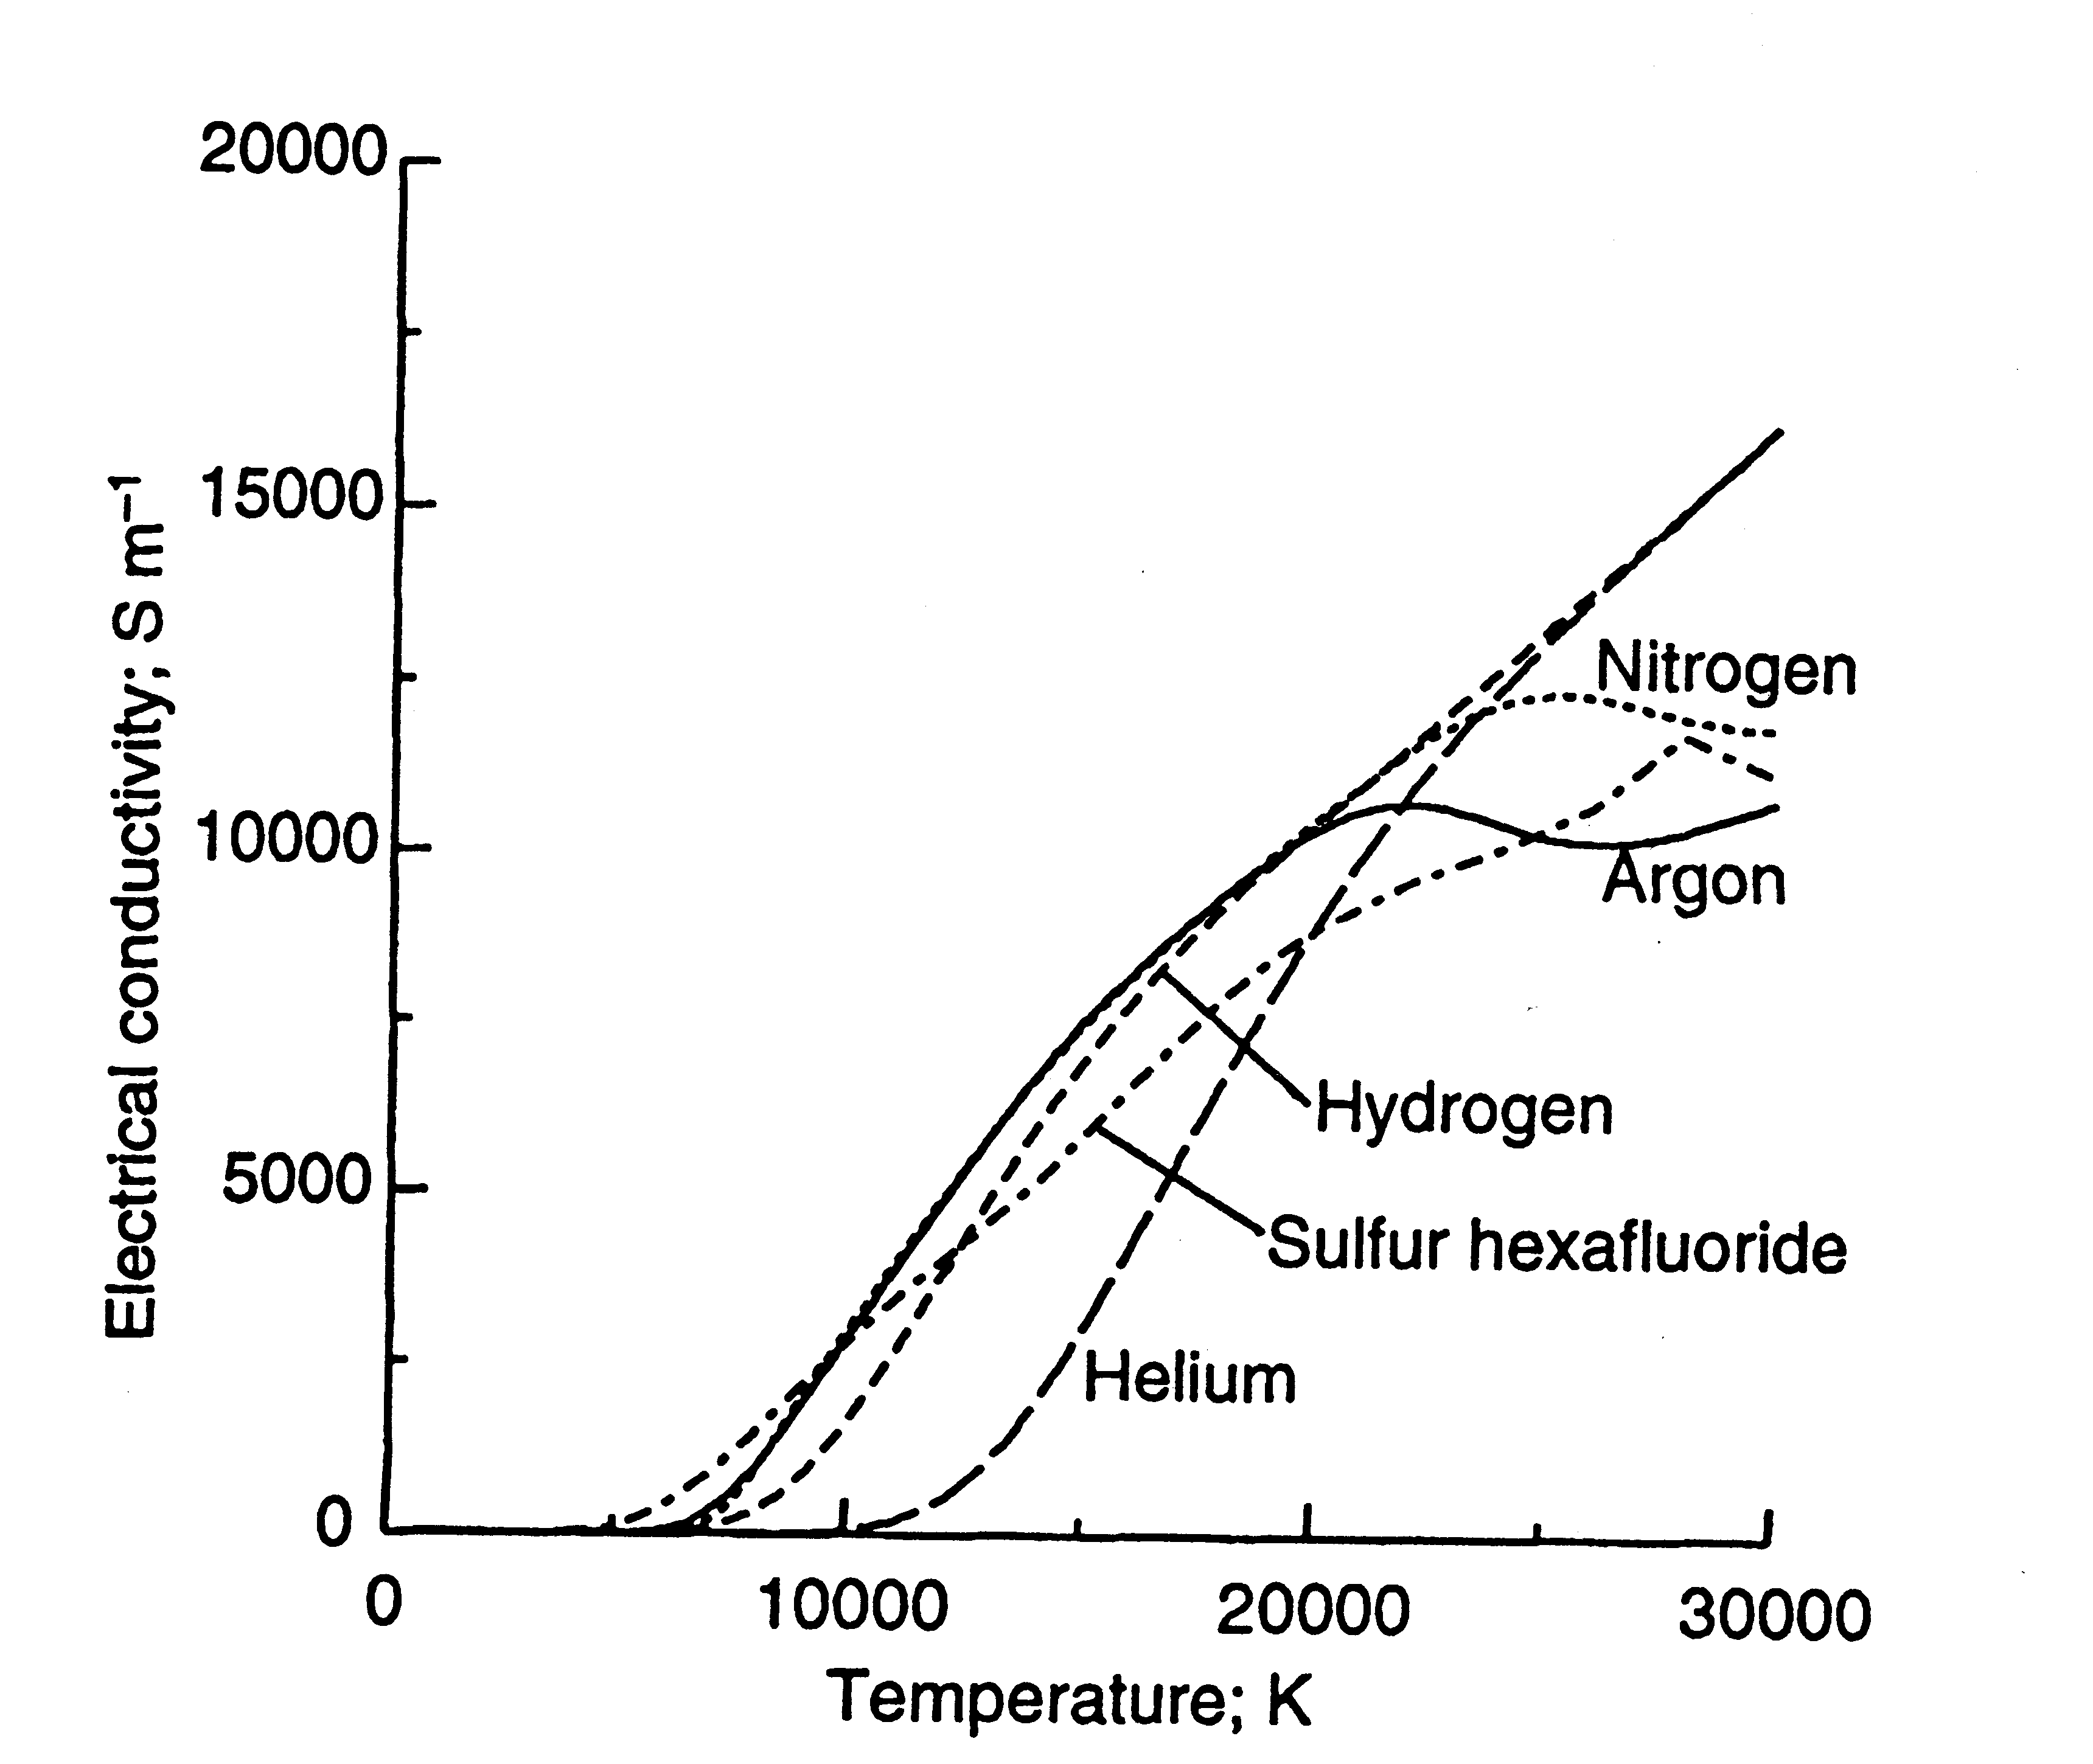
\includegraphics[scale=1]{Bilder/Discussion/conductSF6AndAIR.png}
\caption{The conductivity of air and SF${_6}$ \cite{bib:THFD}.} \label{fig:AirandSF6ConComp}
\end{figure}

In figure \ref{fig:AirandSF6ConComp}, the electrical conductivity of air and SF$_6$ is compared. At high temperatures, when both gases are fully ionised, the conductivity is high, almost in the same range as metals. The transaction between the isolating and the conducting stage is fast. If the particle density displayed in figure \ref{fig:Ndensi} and \ref{fig:SF6densi} of the two gases is taken into account, it is possible to observe that the decomposition of SF$_6$ occurs at a lower temperature than nitrogen. This can indicate that the transaction from non-conductive to conducting take place a bit faster for SF$_6$ than air. In an LBS this might slightly influence the interruption capabilities, but it is not the electrical conductivity that is the main difference and challenge for SF$_6$ and air as an interrupting medium. Both SF$_6$ and air have fairly good electrical conductivity profiles for interrupting currents.

As the current magnitude approaches zero, and the gases recombine, SF$_6$ has one major advantage that air does not. Decomposed SF$_6$ consists of a high concentration of ionised fluorine, both F$^{+}$ and F$^{++}$. These particles are considered to be highly electron negative, which means they will attract electrons. In the moment right after CZ, there are a lot of free electrons in the gap between the contact plates. It is essential to remove these fast to avoid thermal re-ignition of the electrical arc. In an SF$_6$ based switchgear, many of these free electrons are absorbed by the ionised fluorine. In air, oxygen has this effect but the concentration of ionised oxygen is far lower than fluorine. This is one of the reasons that makes thermal re-ignition a larger problem for an air-based switchgear than in an SF$_6$-based system.

\subsubsection*{Thermal conductivity}
When regarding current interruption and the possibility for thermal re-ignition, it is the thermal conductivity that differs the most between air and SF$_{6}$. From figure \ref{fig:tempConGas} in section \ref{sec:HeatTransport}, this difference is pointed out. For the temperature ranges that can be expected in a typical LBS during the high current stage of the interrupting process, air has a fairly high thermal conductivity, while SF$_6$ has a low one, giving SF$_6$ a clear advantage over air. The most critical part in an interruption is how the interruption medium behaves the moment right before CZ. It is in the temperature range that occurs at this stage of the interruption the biggest challenge with using air as an interruption medium applies.

When the current amplitude is rising or is high, the temperature in the plasma channel will be high due to energy dissipation in the arc. At this stage in the interruption process, it is preferred to have an interrupting medium with a low thermal conductivity. A low thermal conductivity will ensure that the energy is stored in the arc, thereby increasing its temperature even more rather than dissipating it out to the surroundings. At high temperatures, SF$_6$ has a fairly low thermal conductivity while air has a high one. The high thermal conductivity of air in this temperature range might result in a poorer electrical conductivity due to temperature loss, which again may result in a slightly higher arcing voltage. The high thermal conductivity of air and the larger energy dissipation will result in heating of the surrounding gas. The gas surrounding the arc might act as an energy buffer, storing heat, which is making the plasma channel more resistant to fast changes in temperature, setting higher demands for the cooling mechanism in the switchgear when using air instead of SF$_6$.

Even though the difference in thermal conductivity at high temperatures is a challenge when dealing with air instead of SF$_6$, it is the difference in the heat transportation properties at lower temperatures that is the most challenging. At the moment right before CZ, it is an advantage that the thermal conductivity of the gas is high. This is because the current amplitude is low and falling, and due to the high thermal conductivity the energy in the plasma channel is transferred out to the surroundings fast. This results in a temperature drop in the arc. The speed of the temperature drop will depend on the temperature of the surroundings and the thermal conductivity of the gas. As the arc extinguishes and the current is zero, it is crucial that the ionised gas recombines to avoid re-ignition. The recombination rate is dependent on the temperature of the gas.
 
Since SF${_6}$ has a high thermal conductivity for temperatures that will occur around CZ, the gas will cool down quickly and recombine fast. Air will nonetheless use longer time than SF${_6}$ to cool down and recombine, due to its low thermal conductivity at this stage in the interruption process. This means that in the moment right after CZ there will be a lot of ionised air particles between the contact plates, but in an SF${_6}$-based breaker more of the gas has recombined. This property will result in a higher chance of thermal re-ignition in an air-based breaker, and put stronger demands on the cooling mechanism.

\subsubsection*{Dielectric properties} 

Even though this research project is mainly focused on thermal re-strikes in an LBS, a few things should be mentioned about the difference in dielectric properties between SF${_6}$ and air. Figure \ref{fig:breakDownVoltage} indicates the different breakdown voltages for SF$_6$ and air for a gas-filled gap at 1 mm with a homogeneous electrical field. As the figure points out, SF$_6$ has a much higher breakdown strength than air, approximately three times higher, but this depends on the gas pressure.

\begin{figure}[H]
\centering
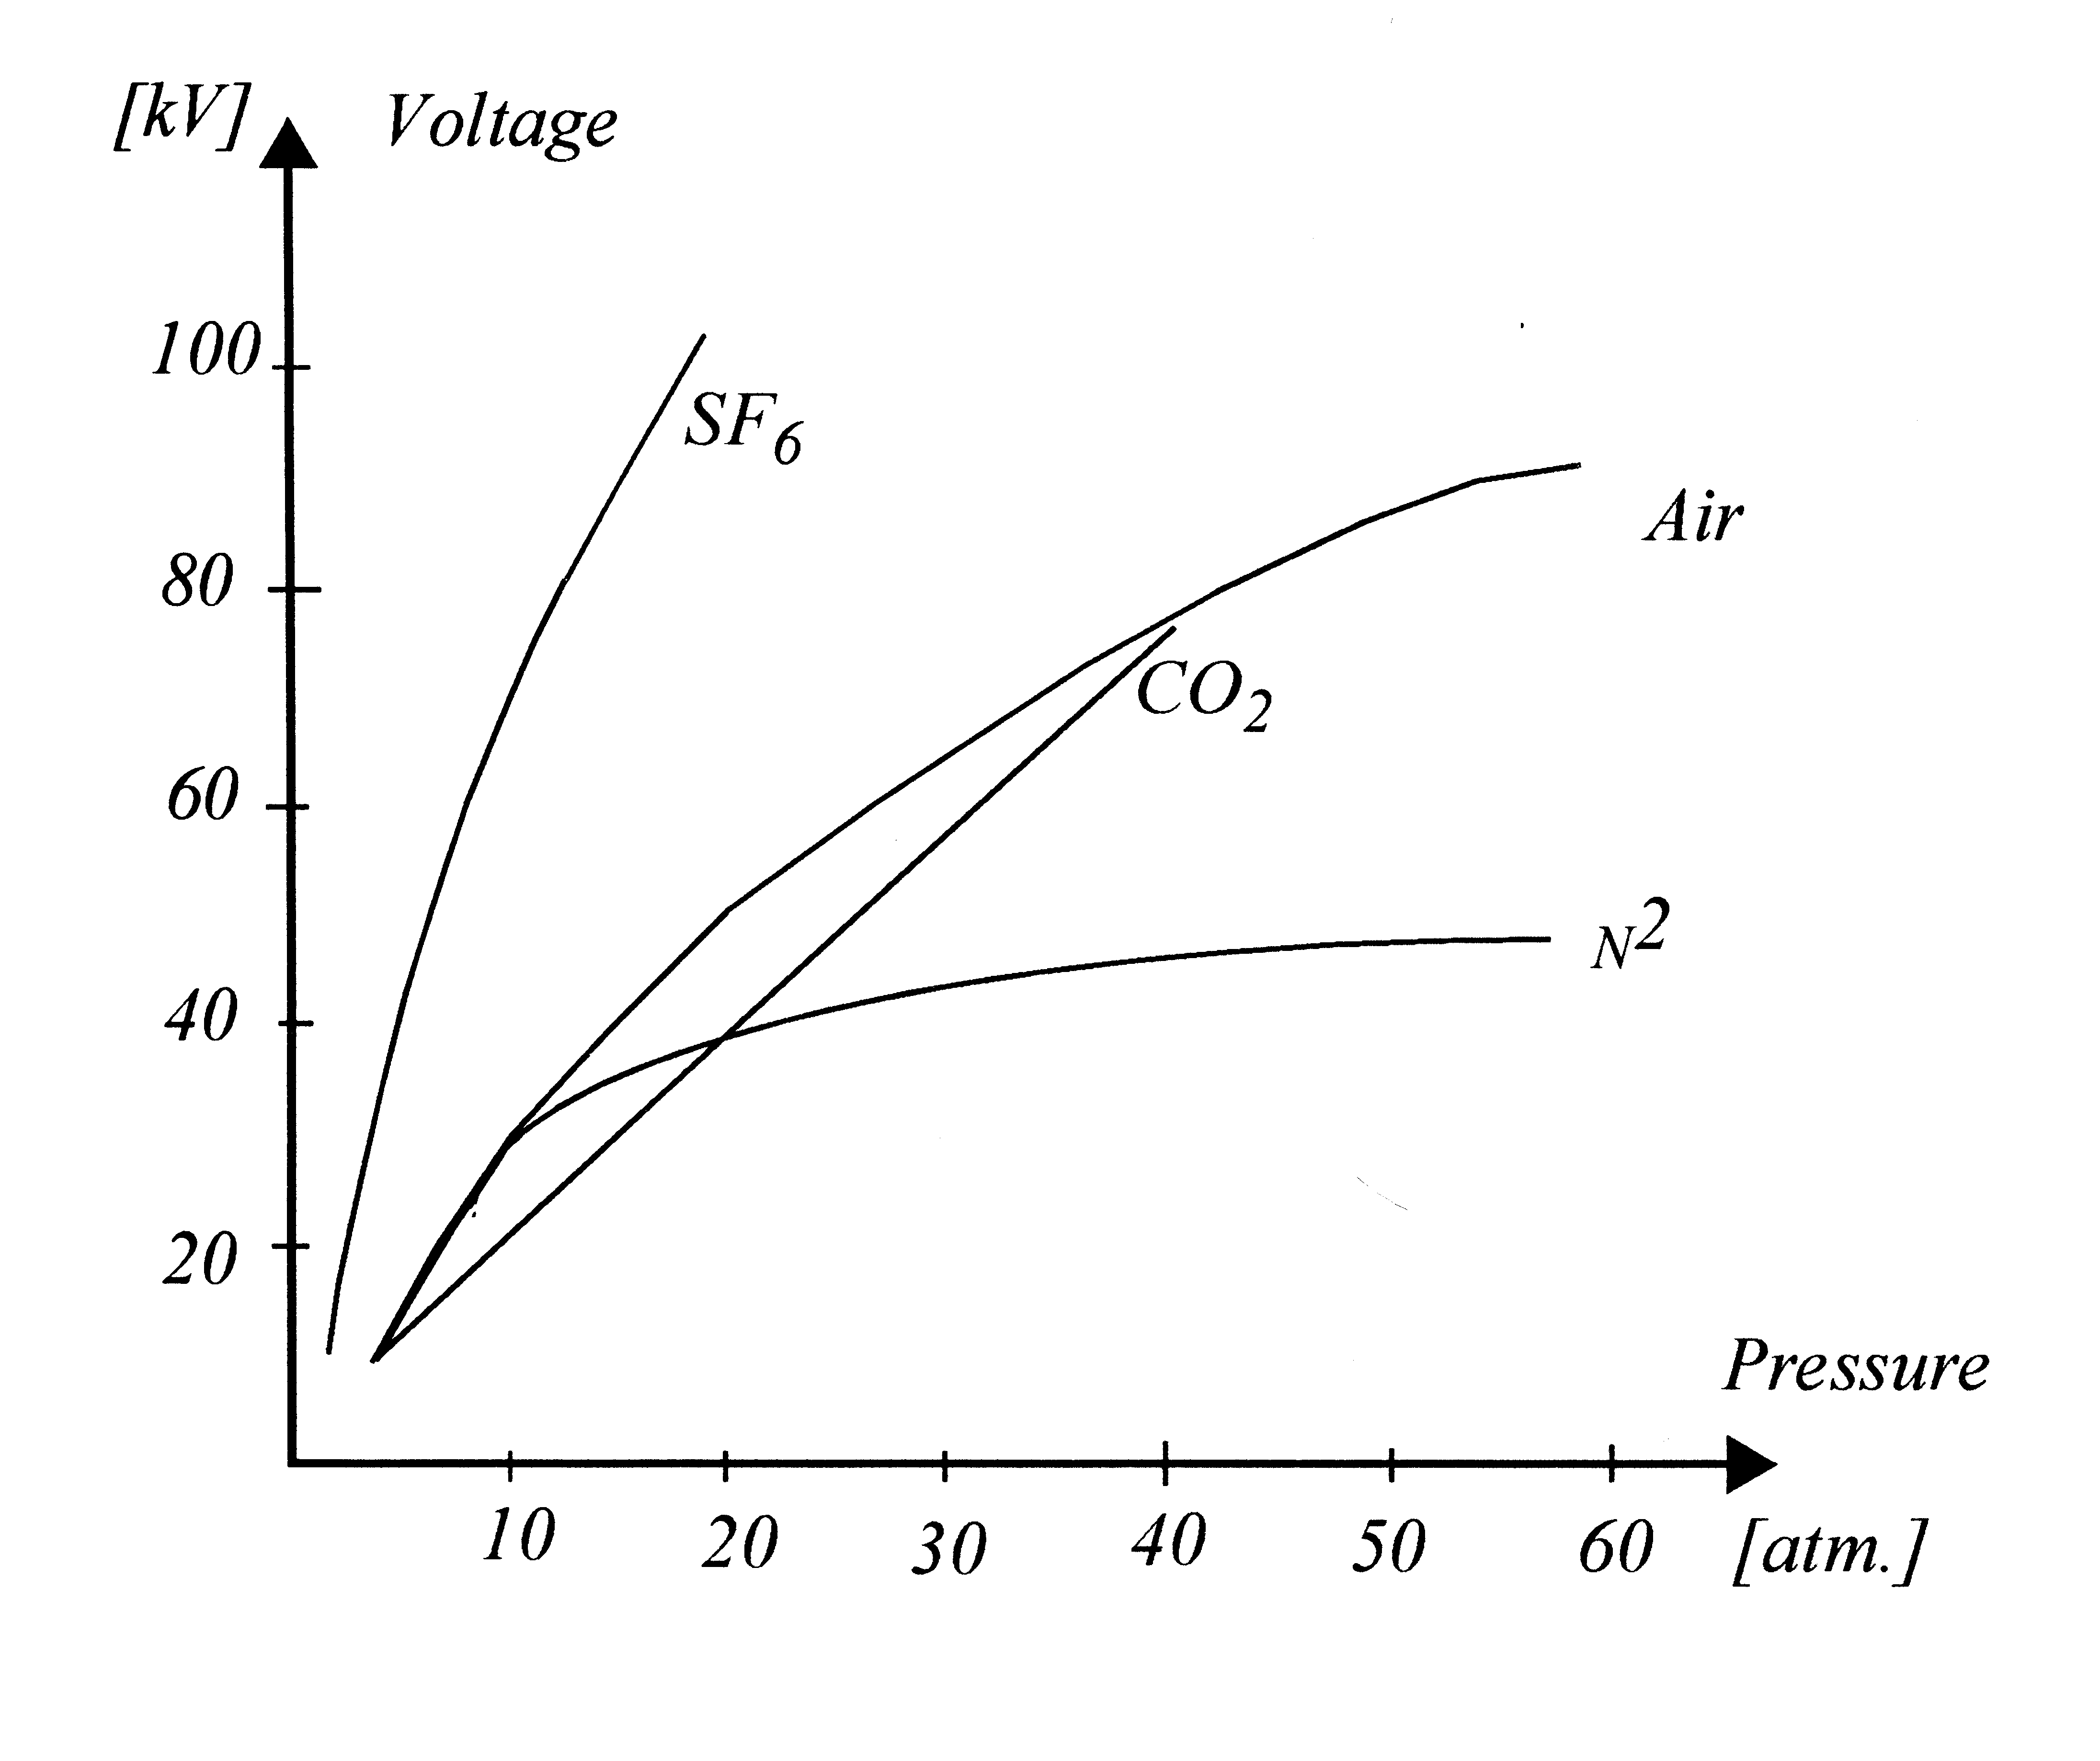
\includegraphics[scale=1]{Bilder/Discussion/Breakdown_voltage.png}
\caption{Breakdown voltage compared to pressure for different gases in a homogeneous field with a gap space equal 1 mm  \cite{bib:TET4160HVIM}.} \label{fig:breakDownVoltage}
\end{figure}

The huge difference in breakdown voltage is mainly due to the high electron negative properties of SF$_6$. Electron negative gases are complex molecular structures mostly consisting of atoms from the halogen group in the periodic system, usually chlorine or fluorine \cite{bib:TET4160HVIM}. These atoms can easily capture free electrons because they lack one electron in the outer shell, and when capturing an electron they become negatively charged ions. Therefore, it is possible to assume that in an electron negative gas, the concentration of free electrons will be low but due to ionisation of the gas, the density of negative ions will be larger. However, the weight of the negatively charged gas molecule makes it less mobile than the much lighter free electron. This makes the impact from free electrons on breakdown voltage much higher than the impact from ionised molecules, resulting in a high breakdown voltage for electron negative gases.

Nitrogen is an electron positive gas because it tends to give away electrons from its outer shell. Partially due to the high concentration of nitrogen in air and the election positive effect, air's breakdown voltage becomes poorer than the one of SF$_6$.

\subsubsection*{Chemical properties}
Both air and SF$_6$ are chemically well suited for use as an interrupting gas. They are stable, non-toxic, non-flammable, and non-explosive. However, SF$_6$ forms highly toxic and corrosive compounds when subjected to electrical discharges \cite{bib:SF6PI}. If water vapour is present in the SF$_6$ gas, the fluorine in SF$_6$ may react with the hydrogen in water, resulting in the formation of hydrofluoric acid \cite{bib:SF6PI}. Hydrofluoric acid is corrosive and will over time damage the switchgear. Fluorine gas and ionised fluorine also form during electrical discharges. Although highly toxic, the gas is contained in the switchgear and therefore considered safe to use. But in the event of a blow-out, persons in close proximity to the switchgear or inside a building containing a large SF$_6$ insulated system might be exposed to fluorine gas and hydrofluoric acid. Air does represent the same toxicity hazard during a blow-out, but fragments and shockwaves from the explosion are similar to when using SF$_6$ a risk.

In cold climates, SF$_6$ might condensate and be partially liquefied. This may result in a lower breakdown strength \cite{bib:SF6PI}. Air does not condensate under any normal operating temperatures. Usually, the pressure in an LBS is too low for this to be a problem, since it rarely exceeds 1.3 bar overpressure. If condensation problems still occur, it is easily avoided with sufficient heating in the switchgear, and therefore it is not considered a significant problem.

\newpage
\subsection{Environmental impacts of SF$_6$ from electrical power industries} \label{sec:EnvirImp}
%Locally the environmental impact from SF$_6$ based switchgear is low. If contaminants, like air and water vapour, is present in the switchgear highly toxic and corrosive compounds might form when the SF$_6$ is subjected to electrical discharges \cite{bib:SF6PI}. Usually this will only be harmful for the equipment, but can result in danger for personnel in close proximity of the switchgear or inside a building containing a large SF$_6$ insulated system during a blow-out. However SF$_6$ is considered to be a safe and stable compound for use in switchgear. The main environmental impact of SF$_6$ is based on its potential as an green house gas.

SF$_6$ is a highly efficient infrared absorber, and this combined with its chemical inertness, makes it one of the strongest greenhouse gases \cite{bib:SF6PI}. In Norway, SF$_6$ makes up 0.4\% of the total greenhouse gas emissions when measured in CO$_2$ equivalents \cite{bib:KlimaKur2020}. Due to the greenhouse gas potential of SF$_6$, this is a fairly small amount of gas, and the emissions are mostly from leakage in high voltage equipment. In Norway, the use of SF$_6$ is regulated through a voluntary agreement between the user group
and the Environmental Department \cite{bib:KlimaKur2020}. The user group consists of almost all major hydropower and electricity distribution companies, but not all owners of SF$_6$-based equipment take part in the agreement between the user group and the Enivronmental Department.

\begin{figure}[H]
\centering
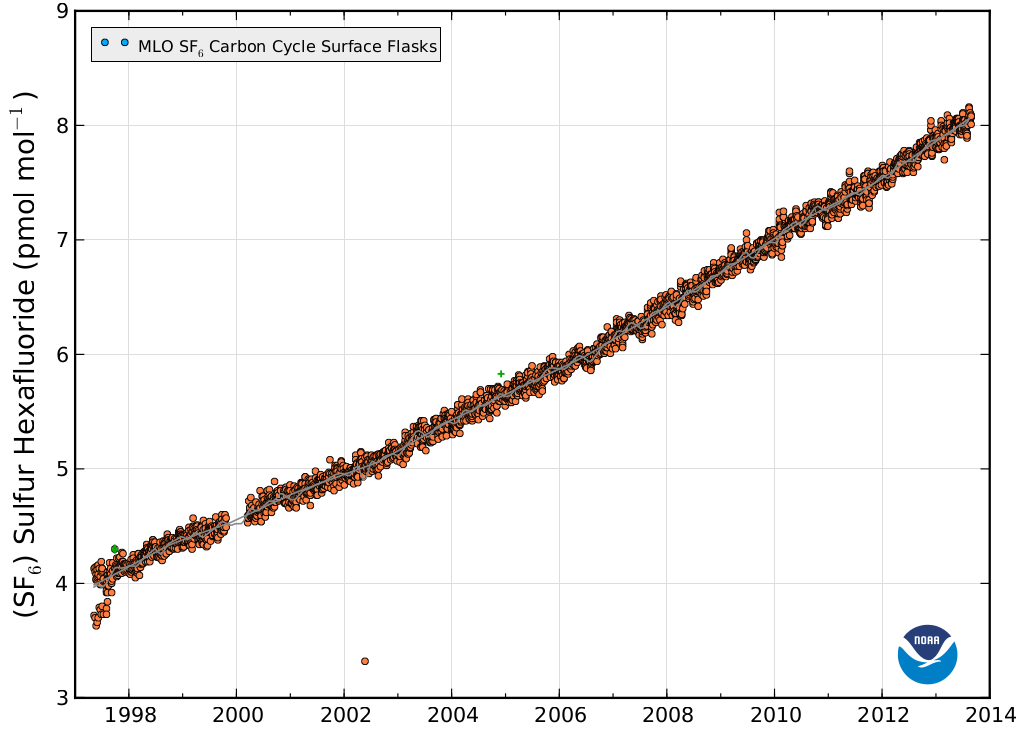
\includegraphics[scale=0.4]{Bilder/Theory/consentrationSF6.png}
\caption{Average SF$_6$ concentration in the atmosphere \cite{bib:consSF6}.} \label{fig:conSF6}
\end{figure}

Because of the increase in commercial use of SF$_6$ since the 1970s, the production of the gas has steadily increased. This has resulted in a rise of the SF$_6$ concentration in the atmosphere, from barely measurable quantities in the 1980s \cite{bib:SF6PI} to relatively high quantities today. In figure \ref{fig:conSF6}, the concentration of SF$_6$ in the atmosphere from 1998 and up until today is indicated. Awareness of SF$_6$ as a potent greenhouse gas has increased in recent years, and as figure \ref{fig:SF6EmissNor} illustrates, the emissions have been reduced by almost half in the period from 2000 to 2003. The voluntary agreement was signed in 2002 and resulted in a methodological change in how emissions were reported in 2003 \cite{bib:regSF6Miljo}. Reports from the industry points at a significant improvement in the handling of SF$_6$ \cite{bib:StatSF6}. It is these two major changes that are the reasons to the apparently huge drop in SF$_6$ emissions from the power industry in Norway between 2000 and 2003.

\begin{figure}[H]
\centering
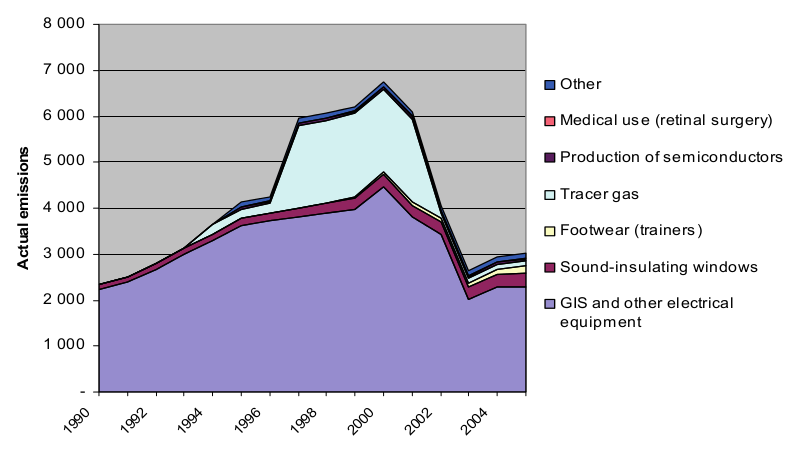
\includegraphics[scale=0.6]{Bilder/Theory/emissionsSF6Norway.png}
\caption{Actual emission of SF$_6$ in Norway \cite{bib:StatSF6}.} \label{fig:SF6EmissNor}
\end{figure}

In 2005, the Norwegian SF$_6$ bank consisted of 202 tonnes of gas. Mostly installed in high voltage switchgear and circuit breakers within the user group members and in addition an estimated 2 tonnes were installed non-members equipment \cite{bib:StatSF6}. Medium voltage switchgear is mainly used by distribution companies and the installed capacity is estimated to be 60 tonnes in 2000 \cite{bib:StatSF6}, of which the user group controls half and the rest is controlled by non-members.

\begin{table}[H]
\center
\caption{Leakage rates from product containing SF$_6$ \cite{bib:StatSF6}.}
\begin{tabular}{|c|c|c|}
\hline 
\textbf{Product emission source}
 & \textbf{Yearly rate of
leakage (per cent)}
 & \textbf{Product lifetime
(years)}
 \\ 
\hline 
Gas-insulated switchgear (GIS)
 & 1 & 30 \\ 
\hline 
Sealed medium voltage switchgear
 & 0.1 & 30 \\ 
\hline 
Electrical transformers for
measurements
 & 1 & 30 \\ 
\hline 
Sound-insulating windows
 & 1 & 30 \\ 
\hline 
Footwear (trainers)
 & 25 & 9 \\ 
\hline 
\end{tabular} 
\label{tab:leakageRatesProdSF6}
\end{table}

Table \ref{tab:leakageRatesProdSF6} points out that most of the emissions into the atmosphere are from high voltage switchgear called GIS. This is due to the leakage rate and the installed bank of 202 tonnes of SF$_6$. A fairly low leakage rate and amount of SF$_6$ installed in medium voltage switchgear make greenhouse gas emissions from this post quite low compared to the GIS post.

Since only half of the SF$_6$ bank in medium voltage switchgear is regulated through the Enivronmental Department with the voluntary agreement, it is possible that the government will be more active in regulation of these kinds of equipment if a more "green" technology becomes available. Taxation or partially banning this equipment to gain some control over the use might be done. But as pointed out in table \ref{tab:leakageRatesProdSF6}, most of the SF$_6$ emissions in Norway are from gas-insulated switchgear, mostly used in high voltage installations. These emissions are hard to completely remove, and even if air might be possible to use in a LBS compact design, it is probably not possible to use in most of the high voltage gas-insulated systems. Therefore, the impact in the total SF$_6$ emissions from the electrical power industry will, even if completely phasing out SF$_6$ based medium voltage switchgear, not be significantly reduced. However, it is one of several things that might be done to reduce the SF$_6$ emissions in Norway.

In Norway, handling and leakage control of SF$_6$ is quite good, especially when compared to some other countries. Therefore, it can be argued that the biggest reduction in SF$_6$ emissions will be in other countries where SF$_6$ is not regulated in the same manner. However, this reduction depends on air-based equipment being made available and taken to use. To make this happen it is important that air-based LBSes are equally good or better than its SF$_6$ counterpart to interrupt currents. It must also be economically feasible regarding lifetime, productions, and maintenance costs. Some kind of international agreement to reduce SF$_6$ emissions might also make the air-based breaker more economically feasible on the global market. With this in mind, it is possible to assume that the global SF$_6$ emissions will be reduced if a competitive air-based LBS is developed.

\cleardoublepage

\section{Method} \label{sec:Method}

\subsection{The switch and contact geometry} \label{sec:switchAndContactGeo}

This experiment is conducted using copper-tungsten arcing contacts, polytetraflourelthylene (PTFE) nozzles and air as interrupting medium. It is an open system, with the surrounding air at atmospheric pressure \textit{p$_0$} and a six litre tank with a pre-filled upstream overpressure \textit{p$_u$}, used during the interruption process to quench the arc. It is possible to adjust the upstream pressure, contact speed and position at current zero (CZ) independently, as well as the contact and nozzle geometry. The current and transient recovery voltage (TRV) can be change by changing the parameters of the laboratory test circuit.

\begin{figure} [h]
\centering
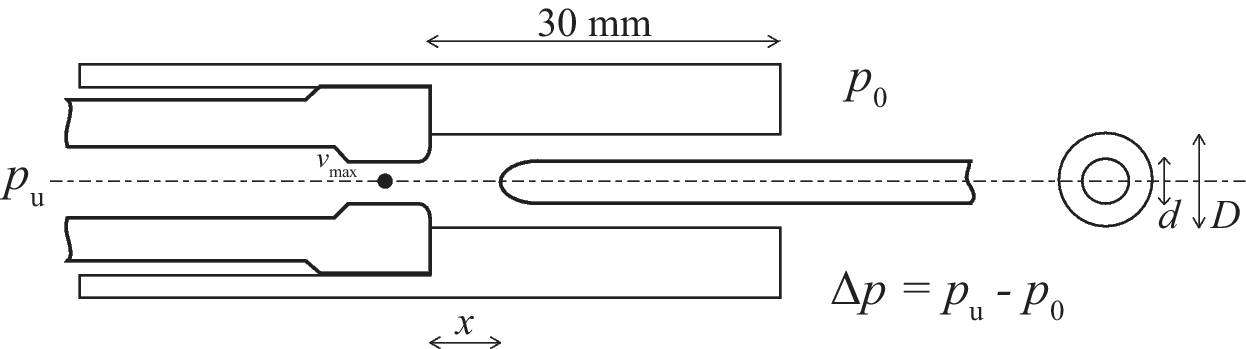
\includegraphics[scale=0.3]{Bilder/Method/contactSetUpVmax3.png}
\caption{The contact and nozzle. The diameter of the contact is \textit{d} and the inner diameter of the nozzle is \textit{D}.} \label{fig:contactAndNozzle}
\end{figure}


A simple drawing of the contact is displayed in figure \ref{fig:contactAndNozzle}. The length of the cylindrical nozzle is 30 mm and the inner diameter is \textit{D}. Two different contact geometries are going to be tested, denoted a and b. The dimensions of the different geometries are illustrated in table \ref{tab:contGeoPara} and how the different dimensions are defined is illustrated in figure \ref{fig:AreacontactAndNozzle}.

\begin{table}[H]
\center
\caption{Contact geometry parameters.}
 \begin{tabular}{|c|c|c|c|c|c|c|}
\hline 
Geometry & D [mm] & d [mm] & $\frac{D}{d}$ & $A_\mathrm{{contact}}$ [mm$^2$] & $A_\mathrm{{ring}}$ [mm$^2$] & $A_\mathrm{{nozzle}}$ [mm$^2$] \\ 
\hline 
a & 10.4 & 4.0 & 2.60 & 12.6 & 72.4 & 84.9 \\ 
\hline 
b & 8.0 & 3.0 & 2.67 & 7.1 & 43.2 & 50.3 \\ 
\hline 
\end{tabular} 
\label{tab:contGeoPara}
\end{table}

The contact position \textit{x} is defined as the axial distance between the tulip and the pin contact. At starting position, \textit{x}= -60 mm, the pin contact is acting as a plug for the tank. This is making it possible to set on upstream pressure. The contact is hold in place by a electromagnet and is set to motion when the magnet releases the contact by a compressed spring. The spring accelerates the pin contact up to a speed of approximately 5.5 m/s at \textit{x}=0. At this position the spring is unloaded  and the pin moves with a constant speed until the contact is fully open at \textit{x}=110 mm.

\begin{figure} [H]
\centering
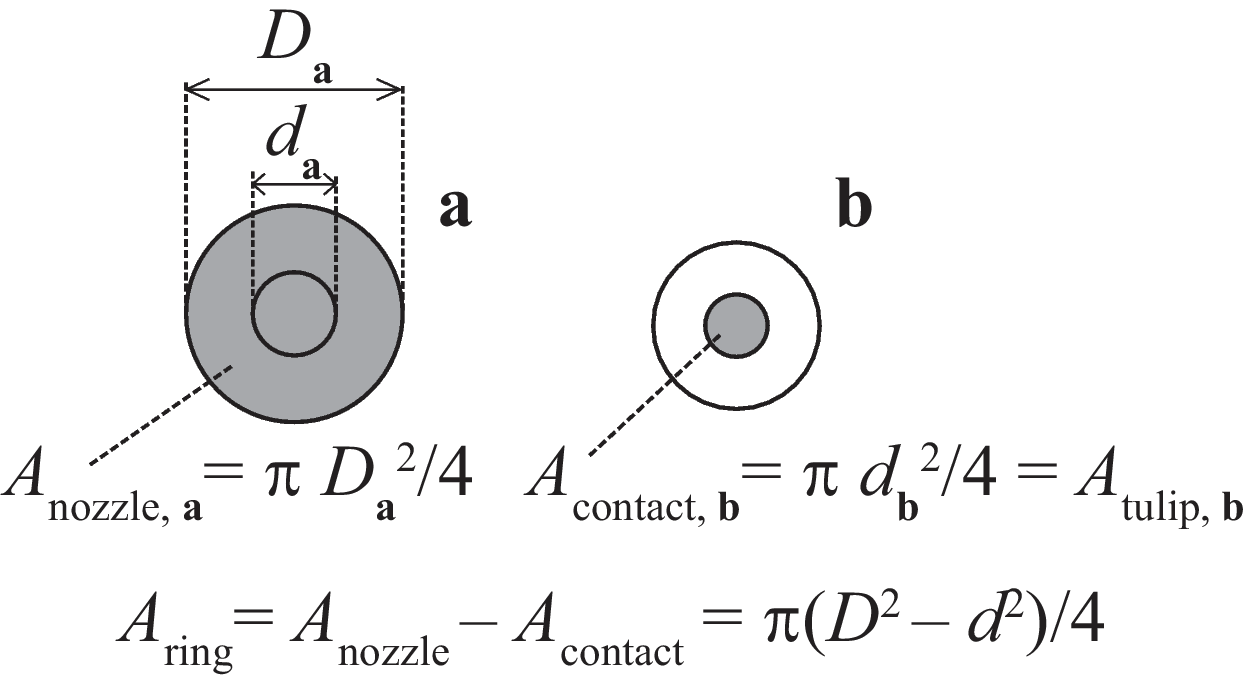
\includegraphics[scale=0.2]{Bilder/Theory/kontaktoversiktAnders.png}
\caption{Overview over how the different areas and diameters are defined.} \label{fig:AreacontactAndNozzle}
\end{figure}

\newpage
\subsection{Test circuit}

\begin{figure} [H]
\centering
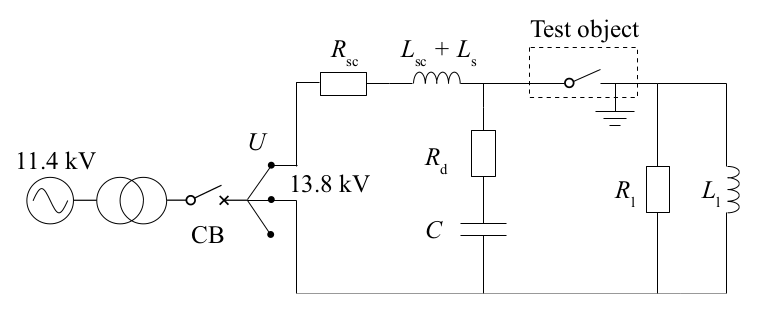
\includegraphics[scale=0.3]{Bilder/Method/circuit.png}
\caption{Circuit used for the interruption test \cite{bib:AFIMVLBA}.} \label{fig:testCurcuit}
\end{figure}

Figure \ref{fig:testCurcuit} is the laboratory test circuit used for the interruption test and supplies 50 Hz / 13.8 kV . It is possible to shape the TRV with tuning the parameters: L$_1$, L$_s$, R$_1$, R$_d$ and C. The systems short circuit parameters are R$_{sc}$ and L$_{sc}$. The TRV generated during interruption is set to simulate the standard for a 24 kV / 630 A class from the International Electrotechnical Commission (IEC) which corresponds to:

\begin{itemize}
\item The initial part of the TRV has a rate of rise in recovery voltage (RRRV) of 71 - 73 V / $\mu$s.
	\begin{itemize}
		\item voltage difference is measured over the first 20 $\mu$s after CZ.
	\end{itemize}
\item The first voltage peak is between 7.0 and 7.4 kV with a rise time of approximately 96 $\mu$s
\end{itemize}

\begin{table}[H]
\center
\caption{Circuit Parameters and Resulting Current \cite{bib:AFIMVLBA}. }
\begin{tabular}{|c|c|c|c|c|c|}
\hline 
L$_s$ [mH] & L$_1$ [mH] & R$_1$ [$\Omega$] & C [nF] & R$_{d}$ [$\Omega$] & I [A] \\ 
\hline 
14.5 & 138.4 & 35.5 & 74 & 248 & 400 \\ 
\hline 
6.9 & 86.2 & 22.1 & 102 & 198 & 630 \\ 
\hline 
\end{tabular} 
\label{tab:testParameters}
\end{table}

In table \ref{tab:testParameters} the value of the different test circuit parameters and the corresponding current can be observed. The test are done at currents with an RMS value of 400 A and 630 A. In all the test the TRV is kept constant up to and including the first voltage peak. In the case of a failed interruption thermal re-ignition occurs within a few microseconds after CZ.

A resistive transducer is measuring the contact position while a Hall effect current transducer is measuring the current through the test switch. The voltage between the contacts is measured with a parallel resistive / capacitive voltage divider. All measurements are transmitted through optical fibres to a 12 bit resolution transient recorder with a sampling frequency is 2.5 MHZ. The pressure in the tank is only measured before each test with an accuracy of 0.01 bar. The test switch is displayed in figure \ref{fig:testSwitchRiggEq}.

\begin{figure} [H]
\centering
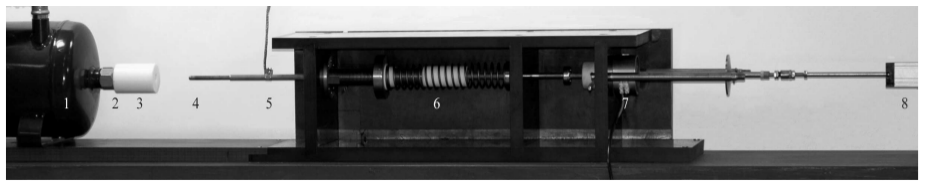
\includegraphics[scale=0.5]{Bilder/Method/switchTest.png}
\caption{Test switch. The numbered parts are: 1. Compressed air reservoir (connected to the high voltage supply circuit), 2. Tulip contact, 3. Nozzle, 4. Pin
contact, 5. Connection to load circuit, 6. Spring drive mechanism, 7. Electromagnet release mechanism, and 8. Position transducer. \cite{bib:AFIMVLBA}.} \label{fig:testSwitchRiggEq}
\end{figure}

\newpage
\subsection{Procedure} \label{sec:procedure}
Interruption tests with CZ occuring both inside and outside the nozzle are carried out. Previous work with a similar setup found that the interruption capability is better outside the nozzle. With two current ratings a total of four cases have been tested, if counting interruptions inside and outside the nozzle as the same case. The first and second CZ is included in this study to provide as much data as possible.

Inside nozzle is defined as contact position x = [5, 25] mm and outside nozzle as x = [35, 60] mm at first CZ. Interruption tests with first CZ either in the vicinity of the tulip contact (x $<$ 5 mm) or in the boundary region between inside and outside the nozzle (x = 25, 35 mm) are not included in the "interruption success rate graphs" but are presented in tables displaying raw data in appendix \ref{app:rawData}. The first CZ occurred within x $<$ 60 mm and the second CZ occurred for x $>$ 60 mm, as the contact speed during all tests was 5.5 mm/ms $\pm$ 0.5 mm/ms.

When testing the interrupting capabilities the test procedure for each of the four cases as follows: 

\begin{itemize}
\item[1.] A pressure level that seems to be in the area of interest is found by performing some initial test interruptions at different pressure levels. This level is kept constant for at least five interruption tests, where all occurred outside the nozzle.
\item[2.] If a pressure level results in less than 100\% successful interruptions, at least five new tests with a higher upstream pressure (next level) is conducted. This is repeated until at least one pressure level with five successful interruptions is found.
\item[3.] Then, the pressure is stepped down until 60\% or more of the interruption attempts fail or the lowest possible pressure level is tested.
\end{itemize}

The pressure level step is 0.1 bar for all tests and at least three pressure levels are tested for each case.\newline

During initial testing it was quickly discovered that the contact geometries were not able to interrupt the current when the pin was inside the nozzle. This resulted in that most of the test where conducted when the pin was outside the nozzle. Therefore at least five tests were performed on every pressure level for the pin outside the nozzle. Some tests at high pressure where performed for each geometry when the pin was inside the nozzle to confirm that it was not possible to interrupt the current for the different geometries.

The arcing voltage is measured and plotted for each test, and saved for further use if an unsuccessful interruption occurs inside the nozzle for geometry \textit{a}. Preferably pressure from 0.6 bar and up to 2.0 bar, with intervals of 0.2 bar is stored.

During the experiments the durability of the contacts are going to be evaluated. When replacing a contact, pictures with a high resolution camera are taken and the number of interruptions are noted. 

The pin is cleaned, polished, and greased between each test to ensure a smooth surface. The contacts and nozzle are replaced regularly to avoid contact wear and nozzle deformation. This is to ensure that the geometry is constant through the whole experiment.

\subsection{Air flow considerations} \label{sec:AirFlow}
 Most of the information in section \ref{sec:AirFlow} is collected from the article \textit{"Air Flow Investigation for a Medium Voltage Load Break Switch"} by N. S. Aanensen, E. Jonsson, and M. Runde \cite{bib:AFIMVLBA}. \newline

From Bernoulli's equation it can be deduced that the maximum velocity of the gas flow through is obtained from a set pressure difference, $\Delta$\textit{p}, as given in equation \eqref{eq:Bernoulli}.

\begin{equation} \label{eq:Bernoulli}
v_{max}=\sqrt{ \frac{2 \Delta p}{\rho}}
\end{equation}

Where $\rho$ is the mass density of the fluid and the fluid is assumed to have an ideal flow without viscosity and incompressible behaviour. The velocity of the gas, $v_{max}$, will occur on the narrowest part of the geometry as indicated in figure \ref{fig:contactAndNozzle}. Since the volumetric flow rate of the gas must be constant the velocity in the other parts of the nozzle can be calculated by the relationship between volumetric flow rate \textit{Q} and $v_{max}$ which is presented in equation \eqref{eq:flowRate}.

\begin{equation} \label{eq:flowRate}
Q=v_{\mathrm{max}} A_\mathrm{{contact}}
\end{equation} 

If table \ref{tab:contGeoPara} is consulted it indicates that the area $ A_\mathrm{{contact}}$ is smaller than both $A_\mathrm{{ring}}$ and $A_\mathrm{{nozzle}}$ for both geometries. This means that for the geometries in this experiment, $v_\mathrm{{max}}$ is always set by the area of the tulip contact and the gas velocity will be the same whenever the pin is inside or outside the nozzle. This is because the volumetric flow is constant. The velocity of the gas that flows in the nozzle is set by equation \eqref{eq:VolumetricFlow}. In figure \ref{fig:AreacontactAndNozzle} the different areas are indicated.
\begin{equation*}
Q=v_\mathrm{{max}} A_\mathrm{{contact}} = v_\mathrm{{nozzle}} A_\mathrm{{nozzle}}
\end{equation*}


\begin{equation} \label{eq:VolumetricFlow}
v_\mathrm{{nozzle}}= v_\mathrm{{max}}\frac{A_\mathrm{{contact}}}{A_\mathrm{{nozzle}} }= v_\mathrm{{max}} \left(\frac{d}{D}\right)^2
\end{equation} 

This indicates that $v_\mathrm{{nozzle}}$ is approximately the same for geometry \textit{a} and \textit{b} since the fraction $D/d$ form table \ref{tab:contGeoPara} is almost the same for both geometries. The volumetric flow rate will increase with the increasing geometry size according to A$_\mathrm{{contact}}$. For pressure differences above 0.7 bar it is expected that sonic speeds can be reached by the gas flow.

The deduction above is based on the assumption that the fluid is non-compressible and has an ideal flow without viscosity. This is probably not valid since turbulence, wall effects, variations in density, and temperature are likely to be present. Without regard to this, these simplifications makes it possible to analyse the air flow in the geometries to a certain extent, and might give the possibility to explain the difference in interruption capabilities when the pin is inside or outside the nozzle. The assumptions above were verified by simulations of compressible gas flow at ambient temperature which was carried out by Nina Sasaki Aanensen. These simulations confirmed that the two geometries has in fact similar air flow velocity at equal upstream pressure and that the air flow velocity is approximately equal when the pin is inside and outside the nozzle. However, the impact of the arc has not been included in these simulations. It is safe to assume that an burning arc between the contacts will have an impact on the air flow, as it heats both the air and surroundings. This has not been accounted for in the cold flow simulations and therefore these are not expected to be accurate.

\cleardoublepage

\section{Results}
\subsection{Interruption tests} \label{sec:interChance}
Originally the one of the intention with the experiments was to test if an equal air flow velocity when the pin was inside or outside the nozzle in the moment of interruption resulted in a equal probability of interruption. However this hypothesis was dismissed because the results from the initial testing indicated that the switch was unable to interrupt at all when the pin was inside the nozzle. Therefore the test procedure was rearranged and the focus was moved to the area when the pin was outside the nozzle at the moment of interruption. At least five interruption test was done at the relevant pressure levels outside the nozzle as described in section \ref{sec:procedure}. The goal with the experiment is to compare the different geometries to each other with regards to interruption success rate compared to pressure level and current amplitude.

For the interruption tests there are four outcomes, at the first CZ the interruption can succeed or a thermal re-ignition can occur. Given a thermal re-ignition in the first CZ the current can be interrupted at the second CZ or another thermal re-ignition can occur. The end result have two outcomes: success or failure. The outcomes are explained by figure \ref{fig:pilSuccessOfFail}. Besides the outcomes listed, there is a small chance of a dielectric re-ignition. However these are rare and are therefore not included. Experience has also indicated that in practical interruption cases thermal re-ignitions are the most demanding tasks for load break switches in the 24 kV 630 A class \cite{bib:AFIMVLBA}. During testing of geometry \textit{b} at 630 A two re-ignitions occurred that was in the area between thermal and dielectric re-ignition, these was counted as thermal failures.

\begin{figure}[H]
\centering
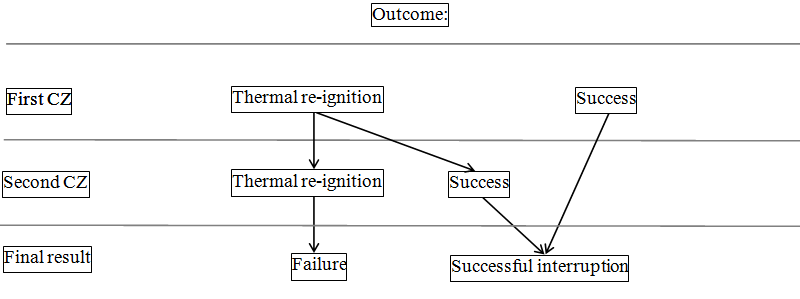
\includegraphics[scale=0.6]{Bilder/Results/interruptionFlowChart.png}
\caption{Flowchart illustrating the different interruption scenarios.} \label{fig:pilSuccessOfFail}
\end{figure}

In figure \ref{fig:CurrentAndVoltageWaveform} the current and voltage during an unsuccessful and a successful interruption are indicated for a 630 A 24 kV test. The upper plot illustrates a thermal re-ignition, as the plot illustrates; the current is almost unaffected of the interruption attempt and continues as normal after the CZ. The lower plot is illustrating a successful interruption, where the current have stopped flowing after CZ and a recovery voltage have raised between the contacts.

\begin{figure}[H]
\centering
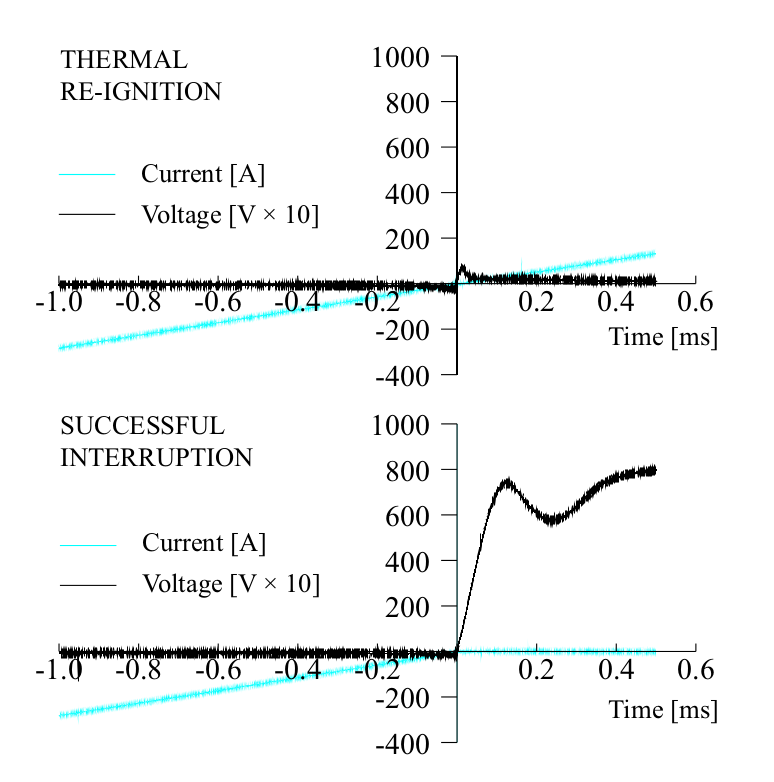
\includegraphics[scale=0.28]{Bilder/Results/differentInterruptions.png}
\caption{Current and voltage waveforms near CZ for two different interruption outcomes \cite{bib:AFIMVLBA}.} \label{fig:CurrentAndVoltageWaveform}
\end{figure}

In figure \ref{fig:successRate400A} the results from the 400 A test for geometry \textit{a} and \textit{b} is presented. The graph are produced with the results from appendix \ref{app:testResults400A}. Figure \ref{fig:successRate630A} points out the results from the two geometries at 630 A, and it is produced from the data in appendix \ref{app:testResults630A}. The data from the boundary regions, which is when the pin are between 25 mm to 35 mm and less than 5 mm away from the tulip contact, is removed from the data selection. Minimum five tests was conducted at each pressure level, and the total probability of interruption are represented as a point in the graph. The exact number of tests at each point is pointed out in the raw data in appendix \ref{app:testResults400A}. It should be noted that in the higher pressure levels only one or two tests at each upstream pressure was done to see if the geometry was able to interrupt currents when the pin was inside the nozzle. Therefore higher variation is expected in the high pressure levels.  

\begin{figure}[H]
\centering
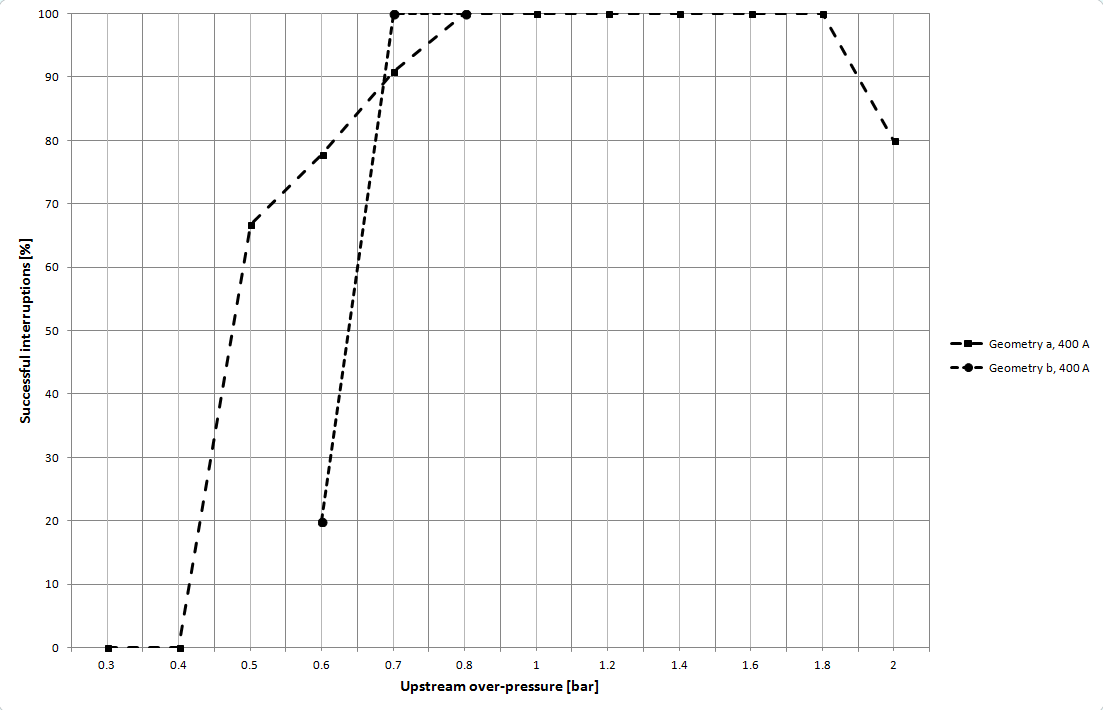
\includegraphics[scale=0.5]{Bilder/Results/successRate400A.png}
\caption{Interruption success rate for geomerty \textit{a} and \textit{b} at 400 A.} \label{fig:successRate400A}
\end{figure}

For the 400 A experiment, geometry \textit{b} performed a little better than geometry \textit{a}. Geometry \textit{b} manages to interrupt 100\% of the tests at a pressure of 0.7 bar, while geometry \textit{a} did this on 0.8 bar. However, geometry \textit{a} manages to interrupt 90\% of the tests at 0.7 bar, resulting in an almost equal performance for both geometries at 400 A.

\begin{figure}[H]
\centering
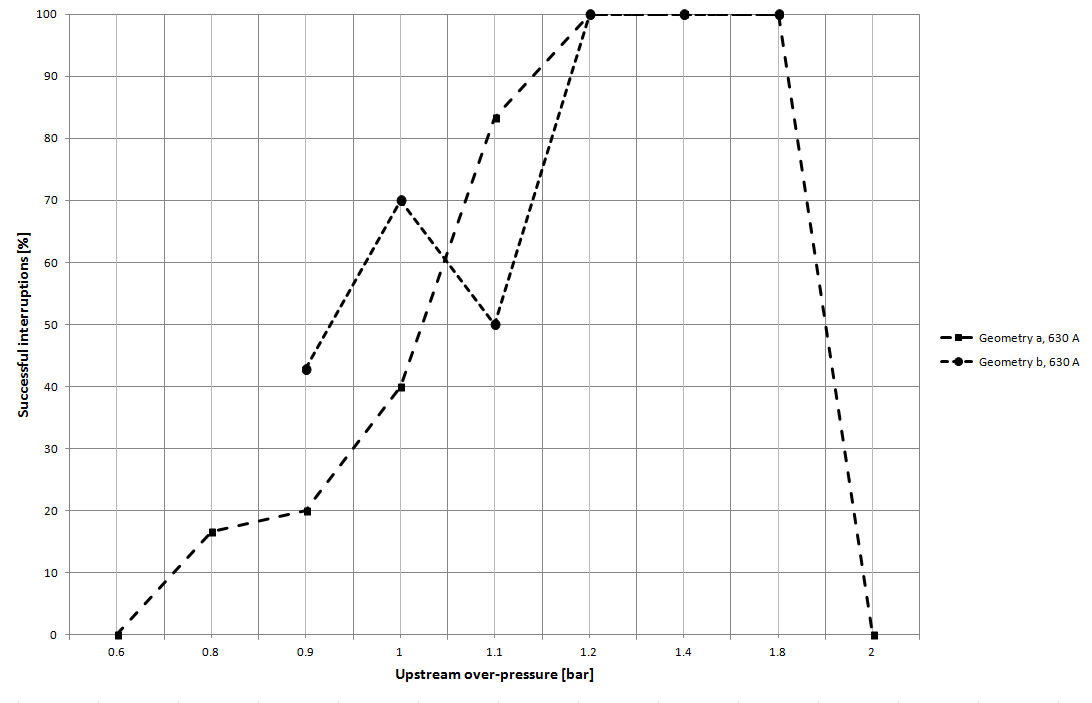
\includegraphics[scale=0.5]{Bilder/Results/successRate630A.png}
\caption{Interruption success rate for geometry \textit{a} and \textit{b} at 630 A.} \label{fig:successRate630A}
\end{figure}

For the 630 A experiment, both geometries successfully interrupted 100\% of the tests at 1.2 bar. However, geometry \textit{a} was more stable and more predictable for each pressure level than geometry \textit{b}. Geometry \textit{b} had more variation in the number of successful interruptions for each pressure level. The variation might have been due to the small dimension of the contact compared to the high amplitude of the current.

Since only a limited amount of tests have been carried out at each pressure level, it is important not to confuse the results presented in this section as statistically proved limits. The results can be regarded as a tool to use in future experiments and may indicate a possible new test geometry. The results can indicate at what pressure level the geometry was able to interrupt or not, but high uncertainties are connected to the percent of successful interruptions and it should not be used as empirical evidence.

The raw data presented in appendix \ref{app:rawData} are presented without alterations. The black line indicates the length of the nozzle and the boundary regions are illustrated with the grey areas. If several tests occurred at the same position in the nozzle, the marker indicating the result has been moved a bit to the side so that the number of tests at each pressure level is countable. For the 400 A experiment, the position measurer was damaged and resulted in an inaccuracy of $\pm$ 2.5 mm for each result. In the 630 A experiment, the the accuracy for the position is set to $\pm$ 1 mm.

\newpage
\subsection{Arcing voltage}
During the experiments, the arcing voltage have been monitored and is presented in figure \ref{fig:arcingVoltage400A} and \ref{fig:arcingVoltage630A}. Each graph illustrates the arcing voltage at a failed interruption when the pin was inside the nozzle at a given pressure. Voltage is indicated along the y-axis and the x-axis indicates time. When CZ occurs the voltages changes polarities and what was before the arcing voltage becomes the TRV. Each voltage plot is shifted along the x-axis a bit so that it is possible to spot the difference between them.

Figure \ref{fig:arcingVoltage400A} displays the arcing voltage for geometry \textit{a} at 400 A. While figure \ref{fig:arcingVoltage630A} illustrates the arcing voltage for geometry \textit{a} at 630 A. There is only one interruption test for each pressure level.

\begin{figure}[H]
\centering
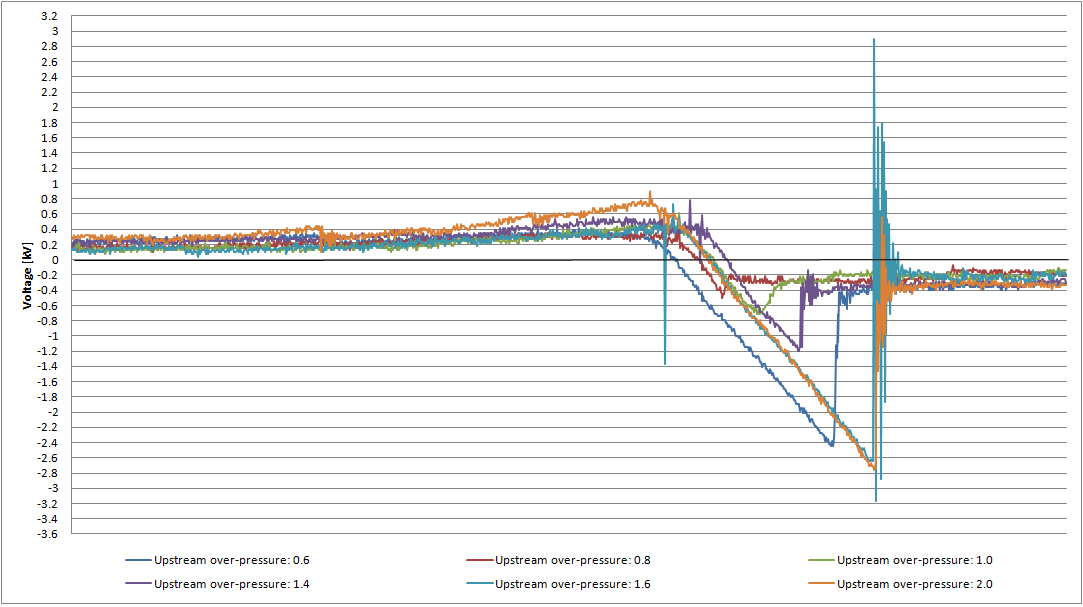
\includegraphics[scale=0.5]{Bilder/Results/arcingVoltage400Ad4.png}
\caption{Arcing voltage for geometry \textit{a} at 400 A for different pressure levels.} \label{fig:arcingVoltage400A}
\end{figure}

\begin{figure}[H]
\centering
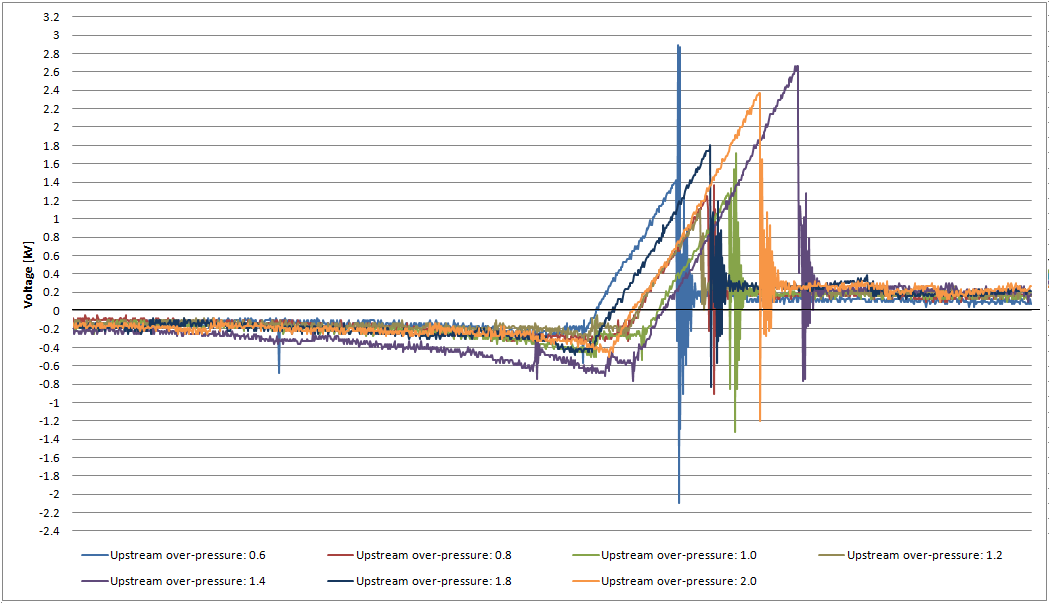
\includegraphics[scale=0.5]{Bilder/Results/arcingVoltage630Ad4.png}
\caption{Arcing voltage for geometry \textit{a} at 630 A for different pressure levels.} \label{fig:arcingVoltage630A}
\end{figure}

\newpage
\subsection{Durability of the arcing contacts} \label{sec:durability}

Since the durability of the arcing contacts was found to be dependent on the current amplitude, some picture of the arcing contacts before and after use is displayed below. A new unused pin contact is displayed in figure \ref{fig:unused_d3}.

\begin{figure}[H]
\centering
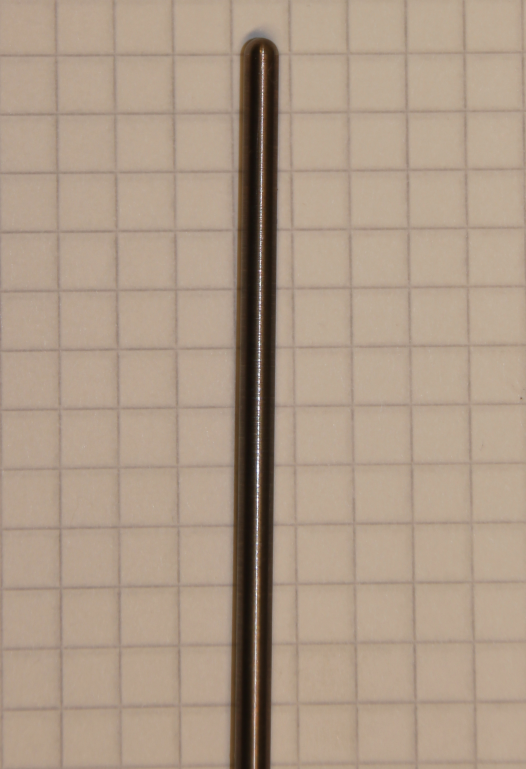
\includegraphics[scale=0.3]{Bilder/Discussion/d3_unused.png}
\caption{Unused male arcing contact of copper-tungsten.} \label{fig:unused_d3}
\end{figure}

For the low current test, with an RMS value of 400 A, both contact diameters handled the wear quite well. The pin that had a diameter of 4 mm was exposed to 82 interruptions. The same pin was also used at the high current test, with an RMS value of 630 A, and was exposed to 37 interruptions. The material in the pin handled this quite well. Despite some sign of damage was observed, this did not seem to have had an impact on the interruption capabilities or the mechanical strength of the pin. The pin after the tests is displayed in figure \ref{fig:d4_burn_side} and \ref{fig:d4_burn_top}. The pin was exposed to both successful and unsuccessful interruptions, therefore a mix of both short and long arcing times.

\begin{figure}[H]
\centering
\begin{minipage}{.5\textwidth}
  \centering
  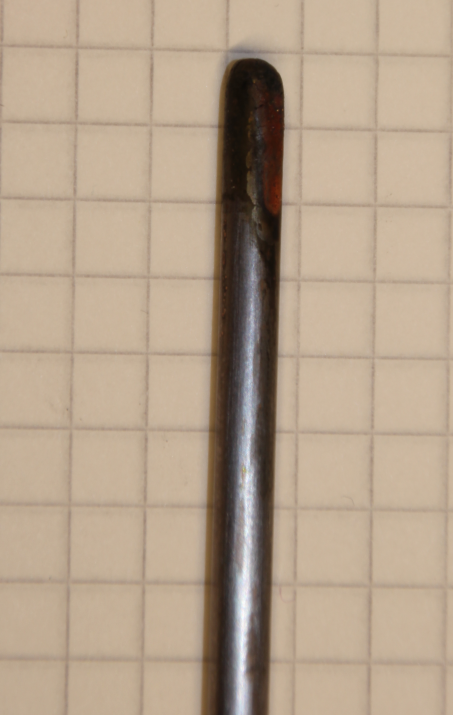
\includegraphics[scale=0.21]{Bilder/Discussion/d4_630and400_burn.png}
  \caption{Pin contact with a diameter of 4 mm, \newline side view.}
  \label{fig:d4_burn_side}
\end{minipage}%
\begin{minipage}{.5\textwidth}
  \centering
  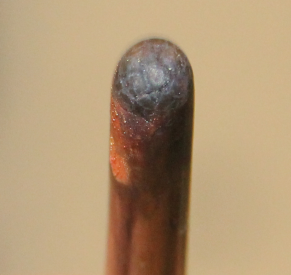
\includegraphics[scale=0.54]{Bilder/Discussion/d4_630and400_top_burn.png}
  \caption{Pin contact with a diameter of 4 mm, \newline top view.}
  \label{fig:d4_burn_top}
\end{minipage}
\end{figure}

The smallest geometry, with a diameter of 3 mm, handled the 400 A test in the same manner as the pin with a diameter of 4 mm. It had signs of wear, but did not needed to be changed during the test and its wear is not assumed to have had an impact on the test result. The smallest geometry is displayed in figure \ref{fig:d3_burn_side} and \ref{fig:d3_burn_top}. This pin was used for five unsuccessful interruptions before it needed to be replaced.


\begin{figure}[H]
\centering
\begin{minipage}{.5\textwidth}
  \centering
  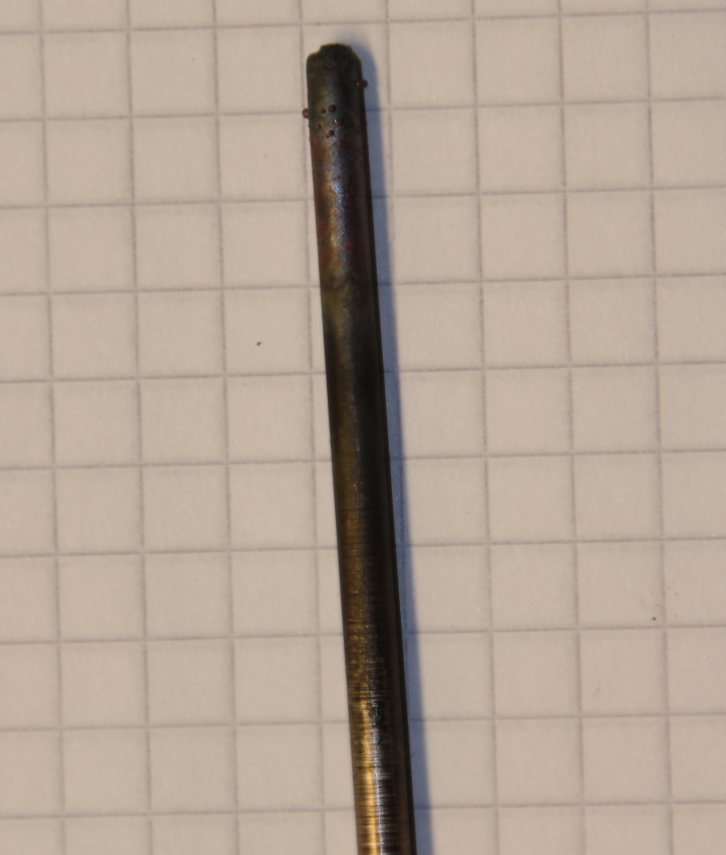
\includegraphics[scale=0.2]{Bilder/Discussion/d3_630_burn.png}
  \caption{Pin contact with a diameter of 3 mm, \newline side view.}
  \label{fig:d3_burn_side}
\end{minipage}%
\begin{minipage}{.5\textwidth}
  \centering
  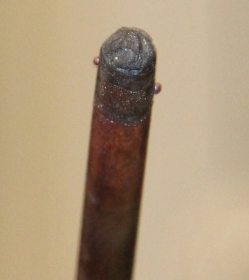
\includegraphics[scale=0.61]{Bilder/Discussion/d3_630_top_burn.png}
  \caption{Pin contact with a diameter of 3 mm, \newline top view.}
  \label{fig:d3_burn_top}
\end{minipage}
\end{figure}

Figure \ref{fig:d3_burn_top} illustrates that droplets of copper that have vaporised from the tip and condensed longer down on the pin. The tip of the pin is severely disfigured and only parts of the tungsten skeleton remains while most of the copper has vaporised from the pin. The interruption results from this test have a lot more variation than the other tests and it might be partially due to the fast wear down of the pin.  


\begin{figure}[H]
\centering
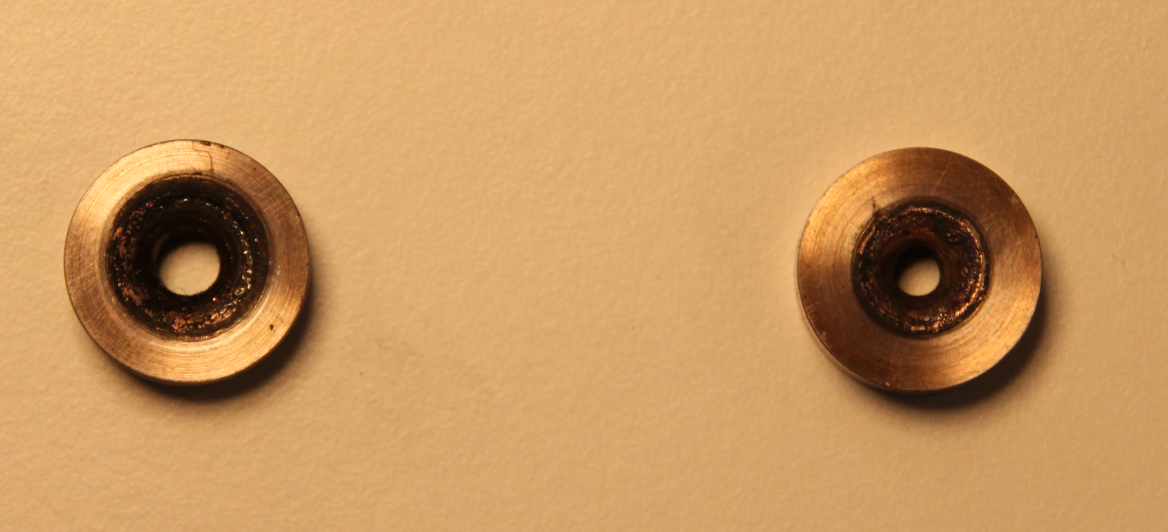
\includegraphics[scale=0.4]{Bilder/Discussion/femaleContacts4mmand3mm.png}
\caption{Used female arcing contact of copper-tungsten. The one to the left has a diameter of 4 mm and the one to the right 3 mm.} \label{fig:used_d4_d3_female}
\end{figure}

As illustrated in figure \ref{fig:used_d4_d3_female}, the tulip contact for both geometries has few signs of wear. None of the tulip contacts were replaced during the experiment, but was polished halfway through each test series to remove soot and other pollution that may have formed on them. The surface area which an arc can burn on is larger for the tulip contact than the pin contact and might be the reason for the much higher durability in the tulip contact than the pin contact.

\cleardoublepage

\section{Discussion}
\subsection{The probability of interruption} \label{sec:DiscIntChan}
When analysing the results presented in section \ref{sec:interChance} it is important to link them to past experiments. A short summary of previous experimental results is presented in appendix \ref{app:PrevReleEx}, and should be consulted when reading this part. For more information regarding past experiments, see article \cite{bib:CIAMVLBS} and \cite{bib:AFIMVLBA}.

Overall geometry \textit{a} performed better than geometry \textit{b} for both interruption test performed in this study. The results from the 400 A interruption test is indicated in figure \ref{fig:successRate400A}. It states that geometry \textit{b} interrupted 100\% of the tests at 0.7 bar upstream pressure, while geometry \textit{a} interrupted 100\% of the tests at 0.8 bar upstream pressure. This is strange considering that geometry \textit{a} has a bigger $A_\mathrm{{contact}}$ than geometry \textit{b}, resulting in a bigger air flow. Geometry \textit{a} has a bigger nozzle diameter than geometry \textit{b}, which might explain that the increase in volume flow of air from geometry \textit{b} to \textit{a} does not result in a improved interruption probability, since the air flow might not be efficiently guided on the arc at 0.7 bar. However, the difference in success rate cannot be considered significant, since the interruption results for geometry \textit{a} at 0.7 bar were 90\%. At an upstream pressure of 0.6 bar, geometry \textit{a} interrupted close to 80\% of the test, while geometry \textit{b} interrupted 20\%. If the 50\% success rate in evaluated geometry \textit{a} performed better than geometry \textit{b}, this is as expected, where \textit{a} had an upstream pressure of approximately 0.47 bar and \textit{b} had an upstream pressure of approximately 0.64 bar. If equation \eqref{eq:Bernoulli} and \eqref{eq:flowRate} is combined, the relationship presented in equation \eqref{eq:flowRateprop} is obtained.

\begin{equation} \label{eq:flowRateprop}
Q \\ \alpha \\ \sqrt{\Delta p} A_\mathrm{{contact}}
\end{equation}

This clearly states that the volume flow \textit{(Q)} will be larger for geometry \textit{a} than geometry \textit{b}, since $A_\mathrm{{contact}}$ is larger when the pressure difference $\Delta p$ is kept constant.

Previous tests have indicated that a nozzle with a small diameter and short length should be chosen. This is because a nozzle too wide may lead to a too low air velocity and may cause the airflow to pass around the arc. However, a too narrow nozzle might cause the arc to clog it and prevent an efficient airflow. The nozzles chosen for this experiment have a diameter of 10.4 mm for geometry \textit{a} and 8 mm for geometry \textit{b}, which is relatively large compared to the pin contact and previously tested geometries. Therefore, it is expected that the current geometries should perform poorer than the test results presented in figure \ref{fig:resultsCIMALBS}.

In figure \ref{fig:ninaBryt}, it can be observed that if the diameter of the pin and nozzle is reduced, higher pressures are needed to perform a successful interruption when the pin is outside the nozzle. This is due to the volume flow which is limited by the smallest cross-section of the contact geometry. For the previous tests presented in appendix \ref{app:PrevReleEx}, $A_\mathrm{{contact}}$ is the limiting cross-section when the pin is outside the nozzle, when the pin is inside the nozzle $A_\mathrm{{ring}}$ is limiting. In the current geometries, $A_\mathrm{{contact}}$ is smaller than $A_\mathrm{{ring}}$ and $A_\mathrm{{nozzle}}$, and is therefore the limiting cross-section. For the tested geometries, $A_\mathrm{{contact}}$ has a diameter of 4 mm for geometry \textit{a} and 3 mm for geometry \textit{b}, which is considerable smaller than previously tested geometries. Hence, it is reasonable to presume that the current geometries should perform poorer than the geometries presented in appendix \ref{app:PrevReleEx}.

If the test results are compared to the results from \ref{fig:ninaBryt}, it follows the same trend as obtained from that experiment. At a current of 400 A, the smallest geometry, which had a contact diameter of 6 mm from figure \ref{fig:ninaBryt}, interrupted all the tests successfully at 0.35 bar upstream pressure. If the 50\% success rate is used, geometry \textit{a} interrupted 50\% of the tests at approximately 0.47 bar upstream pressure, while the one presented in figure \ref{fig:ninaBryt}, denoted as \textit{a}, used 0.2 bar. In equation \eqref{eq:combiGeo}, this geometry is compared to geometry \textit{a} at 50\% success rate based on the difference in volume flow with equation \eqref{eq:flowRateprop}.

\begin{equation} \label{eq:combiGeo}
\frac{Q_{d=6 mm, 50\%}}{Q_{d=4 mm, 50\%}}=\frac{\sqrt{\Delta p_{50\%}} A_{contact, d=6 mm}}{\sqrt{\Delta p_{50\%}} A_{contact, d=4 mm}}
\end{equation}

With numbers inserted in equation \eqref{eq:combiGeo}, this results in a ratio of $\frac{Q_{d=6 mm, 50\%}}{Q_{d=4 mm, 50\%}}\approx 1.5$., which means that geometry \textit{a} uses approximately 1.5 times less air volume than a previously tested design. With the use of equation \eqref{eq:Bernoulli}, the ratio of the maximum air velocity in the contact geometry can be obtained as $\frac{v_{max, d=6 mm}}{v_{max, d=4 mm}}\approx 0.65$. This means that geometry \textit{a} compensates for the 1.5 times smaller air flow with a 1.5 times higher air velocity compared to the smallest contact geometry in figure \ref{fig:ninaBryt}, at 50\% interruption rate. However, the poorer performance of the geometries tested in this experiment is probably not just due to lower volume flow of air but also a lower air velocity inside the nozzle when compared to the other geometries. With equation \eqref{eq:VolumetricFlow}, the ratio of the speed in the nozzle can be calculated to $\frac{v_{nozzle, d=6 mm}}{v_{nozzle, d=4 mm}}\approx 2.5$. This means that when the air flows in the nozzle the air velocity is considerably smaller for geometry \textit{a}. This might partially explain the large difference in needed upstream pressure between the two geometries. The calculations above are only considered as approximations, and the numbers has considerable uncertainties connected to them. This is because the equations are based on cold air flow without an electrical arc, but they might still be used to indicate a difference between the two tested geometries.

Further numerical analysis of these results will not be conducted, and the trends pointed out above will apply to geometry \textit{b} as well. For the other geometries presented in figure \ref{fig:ninaBryt}, the same trends will apply and can therefore be regarded in the same manner. The poorer performance for the geometries in this study was expected when compared to the ones in figure \ref{fig:ninaBryt}. However, for the contact geometries used in this experiment it was hypothesized that: "Since the air velocity when the contact pin is inside the nozzle is the same as when the contact pin is outside the nozzle, it should have approximately the same probability of interruption." This was proven wrong, as none of the tests were able to interrupt the current when the pin was inside the nozzle.

For the geometries discussed above and presented in figure \ref{fig:ninaBryt2}, the volume flow was limited by $A_\mathrm{{ring}}$, since $A_\mathrm{{contact}}$ was larger when the contact pin was inside the nozzle. Due to higher $v_{max}$ but smaller volume flow, it was expected that the geometries tested in this experiment where to perform about equally to the previous tests. Since it was not able to interrupt at all, it might indicate that the interruption rate inside the nozzle is not just based on the speed and volume flow of the air. It is suggested that the area behind the arc is also important for the interruption abilities of contact geometry. This is because it is important during an interruption to not only cool the arc but also remove all charge carriers between the electrodes. When interrupting in air, this is mostly done by a recombination of the ionized air, but there will still be free electrons and metal vapour present even if the air recombines instantly after CZ. The recombination process also uses some time. Therefore, it is essential to physically remove them from the gap between the electrodes. In a puffer concept and in the test switch, this is done by blowing them away. If the area behind the arc is too small, this effect might be less efficient and can hinder the charge carriers being efficiently removed. The area behind the arc is described with $A_\mathrm{{ring}}$ when the contact pin is inside the nozzle.

If $A_\mathrm{{ring}}$ for geometry \textit{a} at 400 A is compared to the previously tested geometry, with a pin diameter of 6 mm at 400 A, the old geometry has a smaller ring area, which is 22 $\mathrm{{mm^2}}$, while geometry \textit{a} has a ring area of 72 $\mathrm{{mm^2}}$, which is relatively large in comparison. Still, no interruptions were obtained. If the volume flow at the 50\% interruption probability for the previously tested geometry is compared to the highest pressure for subsonic air flow for geometry \textit{a} that was tested in this study, when the pin was inside the nozzle, the flow ratio will be: $\frac{Q_{d=6 mm, p=0.23 bar}}{Q_{d=4 mm, p=0.7 bar}}\approx 1.0$. That means that even when blowing with the same volume flow as done before, still no interruptions were obtained. Experiments done with upstream pressure above 0.7 bar were conducted, none of these resulted in a successful interruption either. At this upstream pressure, the air velocity crossed over to sonic speeds. When in the upstream pressure range with sonic speeds, the equations presented in section \ref{sec:AirFlow} are not valid, and a cylindrical nozzle is not suited for these air velocities. Hence, the results from these interruptions are not investigated further. If the same comparison is done to geometry \textit{c} from figure \ref{fig:ninaBryt2}, to geometry \textit{a} from this test, which both have approximately the same ring area, the flow ratio becomes: $\frac{Q_{d=6 mm, p=0.20 bar}}{Q_{d=4 mm, p=0.7 bar}}\approx 2.8$. This might indicate that even when the ring areas are the same, geometry \textit{a} is still blowing with too little volume flow to interrupt the arc.

Since blowing with approximately the same air volume, higher air velocity and using a bigger area behind the arc do not improve the probability of interruption from the previous test, it is difficult to explain why it was impossible to interrupt the current when the pin was inside the nozzle. It is probably due to a combination of the lack of volume flow and the relatively limited area behind the arc. 

When the pin contact was outside the nozzle, it was possible to interrupt the current. However, when compared to previous tests, the lack of volume flow needed to be compensated for with an increased air velocity, resulting in an increase in upstream pressure. The needed pressure is high and not in the pressure range usually applied in commercial load break switches. Nonetheless, it can be argued that in a situation where you have a powerful spring but a limited air volume, it is possible to compensate the lack in volume by increasing the air velocity.

If the results from the 630 A test in figure \ref{fig:successRate630A} is consulted, it can be observed that the pressure needed to obtain more than 50\% successful interruptions are above 0.7 bar and as expected higher than for the 400 A test. However, this means that the air velocity is in the sonic speed range. As mentioned before, the equations applied are no longer valid, and a cylindrical nozzle is not suited. Therefore this results will not be analysed in the same way as the results form figure \ref{fig:successRate400A}. Successful interruptions were obtained when increasing the upstream pressure, which might indicate that when increasing the air velocity, it can compensate for the lack of volume flow. Still, no interruptions were obtained when the pin was inside the nozzle for this current range either. Geometry \textit{b} is still somewhat better than geometry \textit{a} at the 100\% interruption rate but has a faster decline in success rate when the pressure drops. This is the same behaviour as in the 400 A test. For geometry \textit{b}, a fall in the interruption rate from 1 bar to 1.1 bar can be observed. This confirms the trend that high variations are connected to the results obtained through this experiment. The drop at 1.1 bar occurred for reasons unknown, and in figure \ref{fig:rawData630AgeoB}, it can be observed that ten tests were performed at this pressure. The first five tests were performed and all succeeded. Then, as explained in section \ref{sec:procedure}, the pressure was lowered to 1.0 bar and the success rate dropped to 70\%. This was an unexpected drop and five new tests were performed on 1.1 bar where all the tests failed. The pressure was then increased and all the interruptions succeeded. It is assumed that the drop in interruption rate at 1.1 bar was a result of normal statistical variations, but it is also possible that the drop occurred due to damaged contacts. The contacts were closely monitored during the rest of the experiments. This is discussed further in section \ref{fig:durability}.

\subsection{Arcing voltage considerations}
The results presented in figure \ref{fig:arcingVoltage400A} and \ref{fig:arcingVoltage630A} illustrates the arcing voltage during failed interruption tests inside the nozzle at 400 A and 630 A at different upstream pressures. Since each line represents one test, uncertainties are connected to these results, but general trends are pointed out below.

For each experiment the light blue line represents the lowest tested pressure and the orange line represent the highest tested pressure, respectably 0.6 bar and 2.0 bar upstream pressure. The results discussed below are based on a comparison between the highest pressure and lowest pressure. Although some variations can be observed from pressure level to pressure level, both current tests have approximately equal results and little difference can be observed between each current experiments.

When the current has a high magnitude the arcing voltage is approximately the same and constant throughout the whole power cycle, except at the moment the current approaches CZ. An increase in arcing voltage can be observed at this moment and the arcing voltage starts to rise towards its peak. A difference in arcing voltage between the low and high pressure levels can be observed within this time span. For the low pressure test the arcing voltage starts to rise approximately at the same time as the arcing voltage for the high pressure test, but the peaks of the arcing voltage is different. In the low pressure test the arcing voltage have a smaller peak than the high pressure test. It is assumed that the reason for this increase in arcing voltage with increasing pressure is due to how the air flow cools down the arc.

As described in section \ref{sec:HeatTransport} and by figure \ref{fig:tempDist1} it is difficult to cool the arc's core with an air flow, since the temperature in the core is mainly dependent on the current. However, as the current approaches zero the temperature in the core will decrease, as well as the electrical conductivity of the core which is indicated in figure \ref{fig:condAir}. The air flow influence the temperature around the arc with cooling of region two and three in figure \ref{fig:tempDist1}. These regions contains energy in the form of heat, and acts as an energy bank for the core of the arc. When cooling with low pressure difference, the energy stored in these regions is not transported away from the arc as efficient as when cooling with a high pressure difference. This is due to the lower air velocity and volume flow rate. Even though this difference in stored energy has little impact on the temperature in the arc when the current is at high magnitudes it is possible to assume that this energy is important for the temperature in the arc's core when the current approaching CZ, and heating from the current magnitude is less important. If a small amount of energy is stored in the arc's surroundings as in a high pressure test, the transaction from conducting to non-conducting occurs fast. Since the current is mostly controlled by the load side, the change in conductivity will not alter the current magnitude and therefore the raise and peak of the arcing voltage will change with the conductivity of the arc. This is probably the reason for higher peak of the arcing voltage for the high pressure test.

When regarding the impact on arcing voltage from different currents the results are harder to analyse. The arcing voltage seems unaltered and no major change can be observed from the 400 A test and the 630 A test. It might be reasonable to assume that a smaller arcing voltage is expected for higher currents due to a increase in temperature in the arc core. However, due to rising temperature; energy losses from radiation and other factors increases when interrupting in air as mention in section \ref{sec:HeatTransport}, therefore the relationship between arcing voltage and increased current is not easily pointed out. Since the product of current and electrical conductivity determinates the arcing voltage, and the conductivity is highly dependent on the temperature, while the temperature is dependent on the current as well as the thermal conductivity of the gas, it is hard to predict the arcing voltage form one current level to another.

The electrical conductivity in the arc is also dependent on its cross-section. When the current increases the cross-section also increases, this might also influence the arcing voltage since the electrical conductivity in the arc maybe better with an increased cross-section since the current have more space to flow in. However, it can be argued that the arc will be cooled more efficient when the surface area of the arc is bigger, as it would be if the cross-section is increased. The impact from this change in surface area is considered to be small, since the temperature in the arc is not effected by the air flow at high currents. A AC-current with a high amplitude will at some point have the same magnitude as an current with a low amplitude. Even though the magnitude will be the same, the decline will be steeper when approaching CZ for the high amplitude current. This might influence the rise in arcing voltage, making it larger for the high current test, but giving it a equal peak than the low current test. However, this assumption, is hard to point out from the results obtained.

It is reasons to believe that the factors listed below are important to the arcing voltage in an arc, and if the current is increased the electrical conductivity of the arc depend on the following factors: 
\begin{itemize}
\item[] Better electrical conductivity:
	\begin{itemize}
		\item Increased temperature in the arc, due to higher current.
		\item Increased cross-section of the arc, due to higher current.
	\end{itemize}
\newpage
\item[] Poorer electrical conductivity:
	\begin{itemize}
		\item Increased thermal conductivity, due to increased temperature. This tends to lead heat out of the arc and lower its temperature.
	\end{itemize}		 
\end{itemize} 

For the results for geometry \textit{a} these factors seems to compensate for each other and resulting in no significant change in arcing voltage between the two experiments when different current amplitudes was observed. Neither close to CZ or during the normal power cycle of the current. This is backed up by theory which indicates that the arcing voltage is more or less constant from the current magnitudes in the range of 100 A to 1000 A, but dynamic arcs is a complex field of study and many factors applies when determinateing the arcing voltage.

Although the results seems to follow the theory some variations are present. For the 400 A experiment, the 1.4 bar upstream over-pressure test had a higher arcing voltage than the 1.6 bar test. In the 630 A experiment the 1.4 bar test had the highest arcing voltage above 600 V, while the other ones was around 400 V. However variations like this should be expected when only one test is done per pressure level. Since the results from the other pressure tests followed the trend discussed in this section and is supported by the theory presented in this paper these might seems like representative results, further verifications should be done to conclude the trends discussed in this section. It would also be interesting to investigate a connection between the arcing voltage of successful interruptions compared to the arcing voltage of unsuccessful interruptions at the same pressure for the same geometry, both when the pin is inside or outside the nozzle during the CZ as this might give a better insight on what occurs inside the nozzle during the interruption attempt.

The TRV is not discussed in this section, it was assumed that when blowing with high upstream pressure a higher peak in the TRV was going to be observed. The reason behind this is because the switch is closer to successfully quenching the arc. Nonetheless, this was not observed in the results, and more test should be performed before the effect from upstream pressure on the arcing voltage can be pointed out. 

\subsection{Durability of the arcing contacts} \label{fig:durability}

Due to harsh condition during the interruption process it is important that the different parts of the switch is able to tolerate the stress from an arc for several breaking operations and for at least two current zero crossings before the arc is extinguished. As briefly described in section \ref{sec:genDes} and \ref{sec:switchAndContactGeo} the arcing contacts in a LBS consists of different metals or composites designed to withstand the stress from the arc. A common material for the arcing contact is a pseudo-alloy of copper and tungsten called copper-tungsten, this material is also used in the contact-set of the test switch. The main advantage of this pseudo-alloy is that it is able to conduct current quite well because of the good conductivity of the copper, however copper alone will vaporise if exposed to an arc. Tungsten have a high boiling point, and will not vaporise with the same speed as the copper, this makes the contacts more resistant to the stress of the arc. Of the two geometries tested there was a significant difference in the material durability in the pin contact.

The results presented in \ref{sec:durability} might indicate that a small amount of copper-tungsten can be used in the arcing contacts in a commercial LBS, which is good to minimize costs. However it is dependent on the current amplitude since the cross-section and temperature of the arc is highly dependent on the current and it is these two parameters that is assumed to have the biggest impact in the wear of the contact pins. 

Geometry \textit{b} did not tolerate the high current test, and quickly degenerated as displayed in figure \ref{fig:d3_burn_side} and \ref{fig:d3_burn_top}. If figure \ref{fig:tempDist2} is consulted it might indicate that the temperature in the arc have a significant rise from the test with an current RMS value of 400 A to the tests with an RMS value of 630 A. However this increase in the arcs temperature will be experienced by both contact geometries and does not alone explain the significant difference in wear. But geometry \textit{b} will have a smaller surface area where the arc can move along and this difference combined with the increased temperature might have resulted in a faster vaporisation of copper and degeneration of the pin contact for geometry \textit{b}.

Test where the current were interrupted every time was also done with geometry \textit{b}. The degeneration of the pin contact was then slower and less severe. Therefore it might be argued that if a interruption can be guaranteed at the first CZ geometry \textit{b} might also be used to interrupt larger currents. But it should be noted that even if it is possible to successfully interrupt the current on a regular basis without wearing down the pin, a small pin geometry, like geometry \textit{b}, might not be dielectric suitable, especially if air is used instead of SF$_6$ as interrupting medium. A small round shape might be too sharp and can give an enhancement of the electrical field around the tip, resulting in partial discharges and a lower breakdown voltage for the switch design. This might give a problem with spark-overs when the switch is open, due to transients in the power grid, or result in a too long arcing time when closing the switch. Both incidents can be harmful to a fragile arcing contact and may shorten the lifetime of the LBS.
\newpage
\subsection{Suggestion for further work}
\subsubsection{A nozzle that minimizes arc impact on air flow}
Even though none of the geometries were able to interrupt the current when the pin was inside the nozzle, it might seem reasonable to believe that the interruption capabilities should be the approximately equal when the air flow velocity and rate is kept constant no matter the pin's position. Since cold gas simulations have indicated that effects from turbulence, wall effects, variations in density, and temperature are limited it is possible to assume that the impact from the arc is considerable. To minimize this impact it is possible to make the geometries bigger, since the cross-section of the arc is dependent on the current. This will make the arc appear smaller relative to the nozzle geometry, and its impact on the air flow might be limited. In table \ref{tab:contGeoParaNew} a suggestion to a new nozzle design, \textit{c}, is presented and compared to the two tested geometries. If a bigger geometry with the same ${D}/{d}$ is tested it might be possible to know more from the impact of the arc on the air flow, and how the area behind the arc effects the chance for a successful interruption.

\begin{table}[H]
\center
\caption{Contact geometry parameters for a new geometry \textit{c}.}
 \begin{tabular}{|c|c|c|c|c|c|c|}
\hline 
Geometry & D [mm] & d [mm] & $\frac{D}{d}$ & $A_\mathrm{{contact}}$ [mm$^2$] & $A_\mathrm{{ring}}$ [mm$^2$] & $A_\mathrm{{nozzle}}$ [mm$^2$] \\ 
\hline 
a & 10.4 & 4.0 & 2.60 & 12.6 & 72.4 & 84.9 \\ 
\hline 
b & 8.0 & 3.0 & 2.67 & 7.1 & 43.2 & 50.3 \\ 
\hline 
c & 13.0 & 5.0 & 2.60 & 19.6 & 113.1 & 132.7 \\ 
\hline
\end{tabular} 
\label{tab:contGeoParaNew}
\end{table}

\subsubsection{Cone shaped nozzle}
Since the area behind the arc may have an impact on the probability of interruption it might be possible to gradually increase the area behind the arc with a cone shaped nozzle. If a cone shaped nozzle where to be developed it is possible to find the area behind the arc when the pin's position inside the nozzle is known, and then compare it with the interruption success rate. 

A cone shaped nozzle is also considered to guide the air flow better for sonic air velocities, and might improve the interruption rate for high upstream pressures. For the geometries tested in this experiment most of the successful interruptions occurred at sonic speeds. For the reasons mention above, it is believed that a cone shaped nozzle is assumed to performed better than an cylindrical one.

If a cone shaped nozzle where to be developed it should be comparable to an already tested design, or a to be tested design. If it is designed so that $A_\mathrm{{contact}}$ is smaller than $A_\mathrm{{ring}}$ and $A_\mathrm{{nozzle}}$ at all times, it will ensure that the air flow rate and velocity are independent from the pin's position relative to the nozzle. 

\begin{table}[H]
\center
\caption{Contact geometry parameters for a cone design.}
 \begin{tabular}{|c|c|c|c|c|c|}
\hline 
Geometry & D$_\mathrm{{start}}$ [mm]& D$_\mathrm{{end}}$ [mm] & d [mm] & $\frac{D_\mathrm{{start}}}{d}$ & $A_\mathrm{{contact}}$ [mm$^2$] \\ 
\hline 
a & 10.4 & 14.0 & 4.0 & 2.60 & 12.6  \\ 
\hline 
b & 10.4 & 16.0 & 4.0 & 2.60 & 12.6  \\ 
\hline 
\end{tabular} 
\label{tab:contGeoParaCone}
\end{table}

In table \ref{tab:contGeoParaCone} examples of two different contact geometries with a cone shaped nozzle are indicated. They both have the same length of 30 mm, and the same pin diameter of 4.0 mm. D$_\mathrm{{start}}$ represents the diameter at the start of the nozzle close to the tulip contact, while D$_\mathrm{{end}}$ is the diameter at the end of the nozzle. Since D$_\mathrm{{start}}$ is the same and D$_\mathrm{{end}}$ is different for the test geometries the results might illustrate the impact on current interruption from the different areas and increase in the area behind the arc. Which can be compared to the test results from geometry \textit{a} in this experiment, where the area behind the arc is equal no matter the pin's position inside the nozzle, and that there is no increase in the area. Figure \ref{fig:cone_D16} illustrates a cone shaped nozzle with the same  D$_\mathrm{{start}}$ as geometry \textit{a}, but a different D$_\mathrm{{end}}$. 

\begin{figure}[H]
\centering
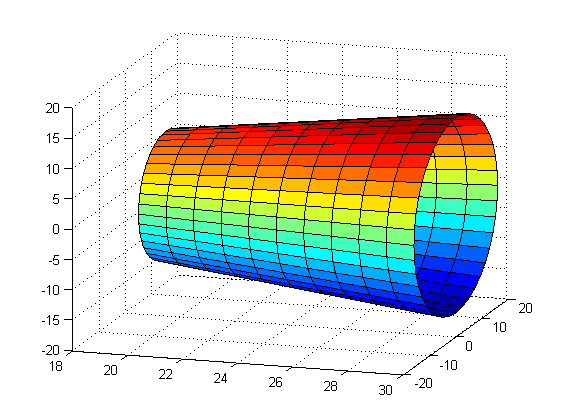
\includegraphics[scale=0.36]{Bilder/Discussion/cone_D16.png}
\caption{Nozzle shaped like a cone.} \label{fig:cone_D16}
\end{figure}

\cleardoublepage

\section{Conclusion}
Interruption tests where carried out for the two geometries \textit{a} and \textit{b}, at different upstream pressures for currents at 400 A and 630 A, and resulted in the following:
\begin{itemize}
\item	It was possible to interrupt the current for both geometries when the pin was outside the nozzle. Compared to previous tested geometries a high upstream pressure was needed, thus proving that a high air velocity can compensate for a smaller volume flow.
\item	None interruptions where obtained when the pin contact was inside the nozzle. Several reasons were investigated, but the cause is unknown. This concludes that even with the same air velocity, $v_\mathrm{{max}}$, whether the pin is inside the nozzle or outside the nozzle, the probability of interruption is not equal. 
\item	A trend where the arcing voltage's peak increases with the upstream pressure was observed, the cause for this is assumed to be increased cooling.
\item Both the pin contacts tolerated the 400 A interruption test quite well. Geometry \textit{a} handled the 630 A test without significant wear, but the pin contact in geometry \textit{b} was quickly degenerated. However it is possible that if interruptions can be guaranteed at the first CZ the pin contact for geometry \textit{b} might be used at 630 A. The tulip contact for both geometries had none significant signs of wear during the experiment.
\end{itemize}

\cleardoublepage
\begin{thebibliography}{10}
\bibitem{bib:SF6PI} L.G. Christophorou, J. K. Olthoff, and R.J. Van Brunt, "Sulfur hexafluoride and the electric power industry", \textit{IEEE Electrical Insulation Magazine, vol. 13, No. 5, pp. 20-24}, Oct. 1997.

\bibitem{bib:comSub} amesimpex.com, \url{http://www.amesimpex.com/images/unitised_sub_002.jpg}, 26.9.2013

\bibitem{bib:HVEbreak} M. Runde, "Current interruption in power grids", Trondheim: Norwegian University of Science and Technology, 2013

\bibitem{bib:CBAC} W. Rieder, "Circuit breakers, physical and engineering problems, III-Arc-medium considerations", \textit{IEEE spectrum, pp. 80-84}, Sept. 1970.

\bibitem{bib:IPSF6AQM} W. Hertz, H. Motschmann and H. Wittel, "Investigations of the properties of SF$_6$ as an arc quenching medium", \textit{Proceedings of The IEEE, vol. 59, NO. 4, pp. 485-492}, April 1971.

\bibitem{bib:TDCIGBB} W. Hermann, "Theoretical description of the current interruption in HV gas blast breakers", \textit{IEEE Transactions on Power Apparatus and System, vol. PAS-96, NO. 5, pp. 1546-1555}, Sept./ Oct. 1977.

\bibitem{bib:THFD} R. W. Johnson, "The handbook of fluid dynamics", Heidelberg: Springer-Verlag GmbH \& Co. KG, 1998.

\bibitem{bib:TET4160HVIM} E. Ildstad, "High voltage insulation materials", Trondheim: Norwegian University of Science and Technology, 2012, August 2012.

\bibitem{bib:KlimaKur2020} "KLIMAKUR2020", Oslo: Klima- og forurensningsdirektoratet, 2010

\bibitem{bib:consSF6} esrl.noaa.gov, \url{http://www.esrl.noaa.gov/gmd/webdata/iadv/ccgg/graphs/pdfs/ccgg.MLO.sf6.1.none.discrete.all.pdf}, 17.10.2013

\bibitem{bib:regSF6Miljo} regjeringen.no, \url{http://www.regjeringen.no/nb/dep/md/dok/regpubl/stmeld/2011-2012/meld-st-21-2011-2012/5/5.html?id=682932}, 21.10.2013

\bibitem{bib:StatSF6} K. L. Hansen, "Emissions from consumption of HFCs, PFCs and SF$_6$ in Norway", \textit{Statistics Norway/Department of Economic Statistics/Environmental Statistics}, 2007.

\bibitem{bib:AFIMVLBA} N. S. Aanensen, E. Jonsson, and M. Runde "Air flow investigation for a medium voltage load break switch", to be published.

\bibitem{bib:CIAMVLBS} E. Jonsson, N. S. Aanensen and M. Runde, "Current interruption in air for a medium voltage load break switch", \textit{IEEE Trans. Power Delivery}, in press.

\end{thebibliography}

\cleardoublepage
\appendix
\vspace*{\fill}
\begingroup
\begin{center}
\huge Appendix
\end{center}
\endgroup
\vspace*{\fill}
\cleardoublepage
\section{Appendix: Test Results} \label{app:rawData}
\setcounter{figure}{0}
\makeatletter 
\renewcommand{\thefigure}{A.\@arabic\c@figure}
\makeatother

\setcounter{table}{0}
\makeatletter 
\renewcommand{\thetable}{A.\@arabic\c@table}
\makeatother

\subsection{400 A geometry \textit{a} and \textit{b}} \label{app:testResults400A} 
\begin{figure}[H]
\centering
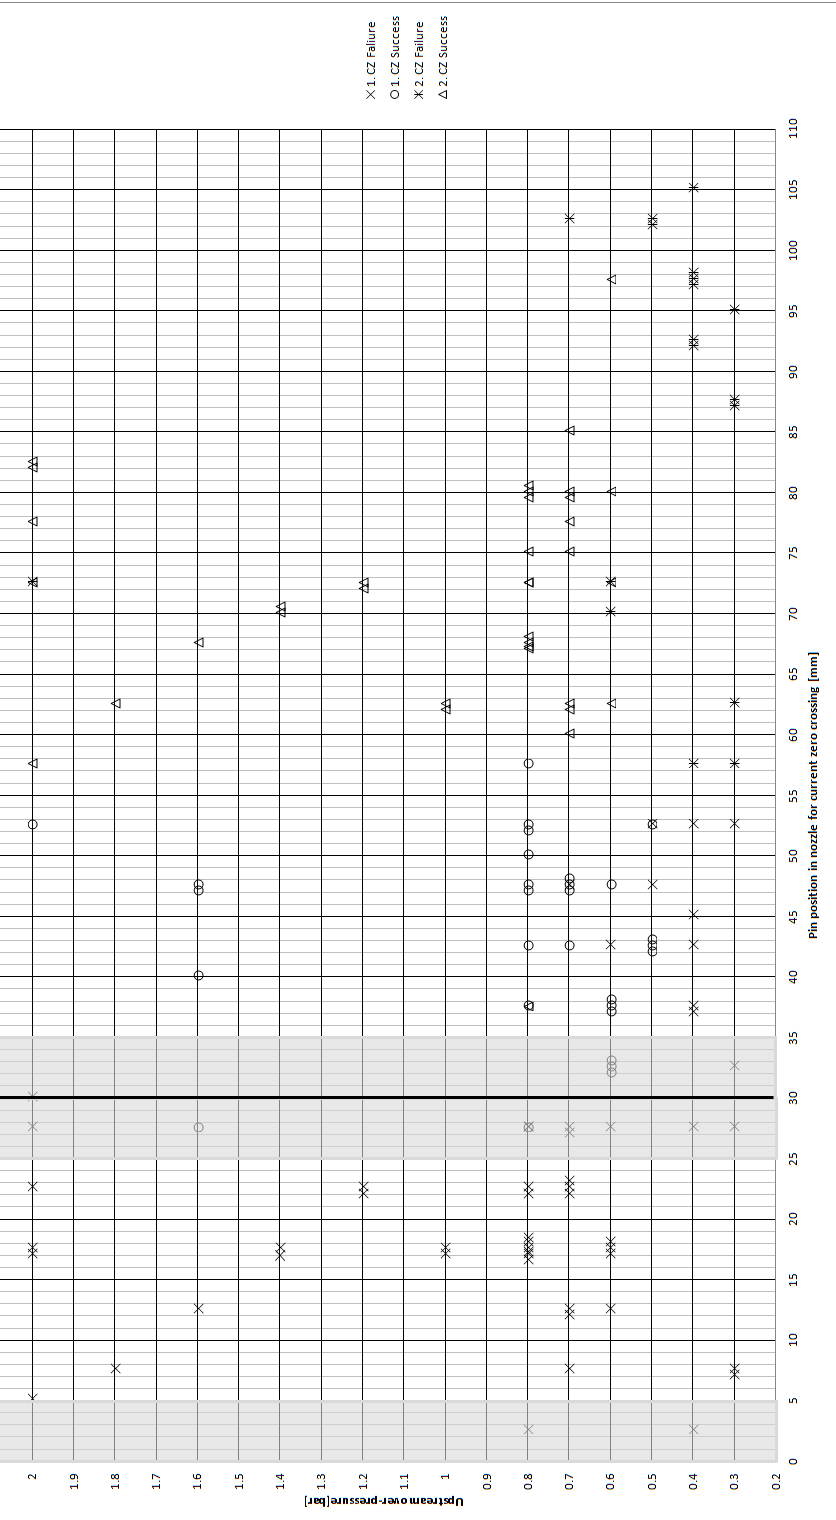
\includegraphics[scale=0.55]{Bilder/Results/rawData400AgeoA.png}
\caption{Raw data for geometry \textit{a} at 400 A, The grey areas are the boundary region where results was discarded for the success rate graphs. The black line indicates where the length of the nozzle.} \label{fig:rawData400AgeoA}
\end{figure}
\newpage

\begin{figure}[H]
\centering
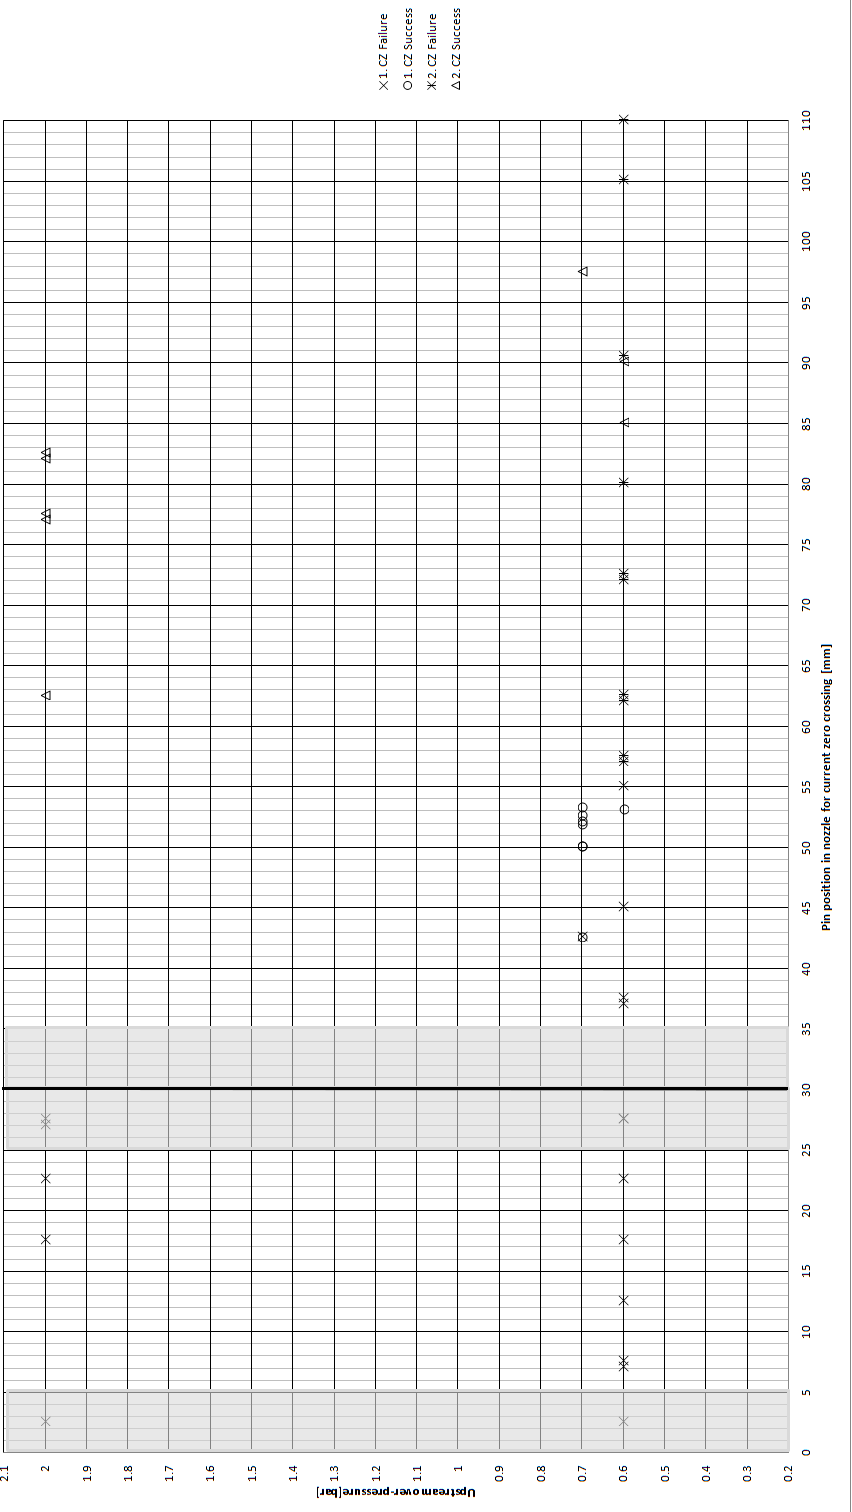
\includegraphics[scale=0.55]{Bilder/Results/rawData400AgeoB.png}
\caption{Raw data for geometry \textit{b} at 400 A, The grey areas are the boundary region where results was discarded for the success rate graphs. The black line indicates where the length of the nozzle.} \label{fig:rawData400AgeoB}
\end{figure}
\newpage

\subsection{630 A geometry \textit{a} and \textit{b}} \label{app:testResults630A}
\begin{figure}[H]
\centering
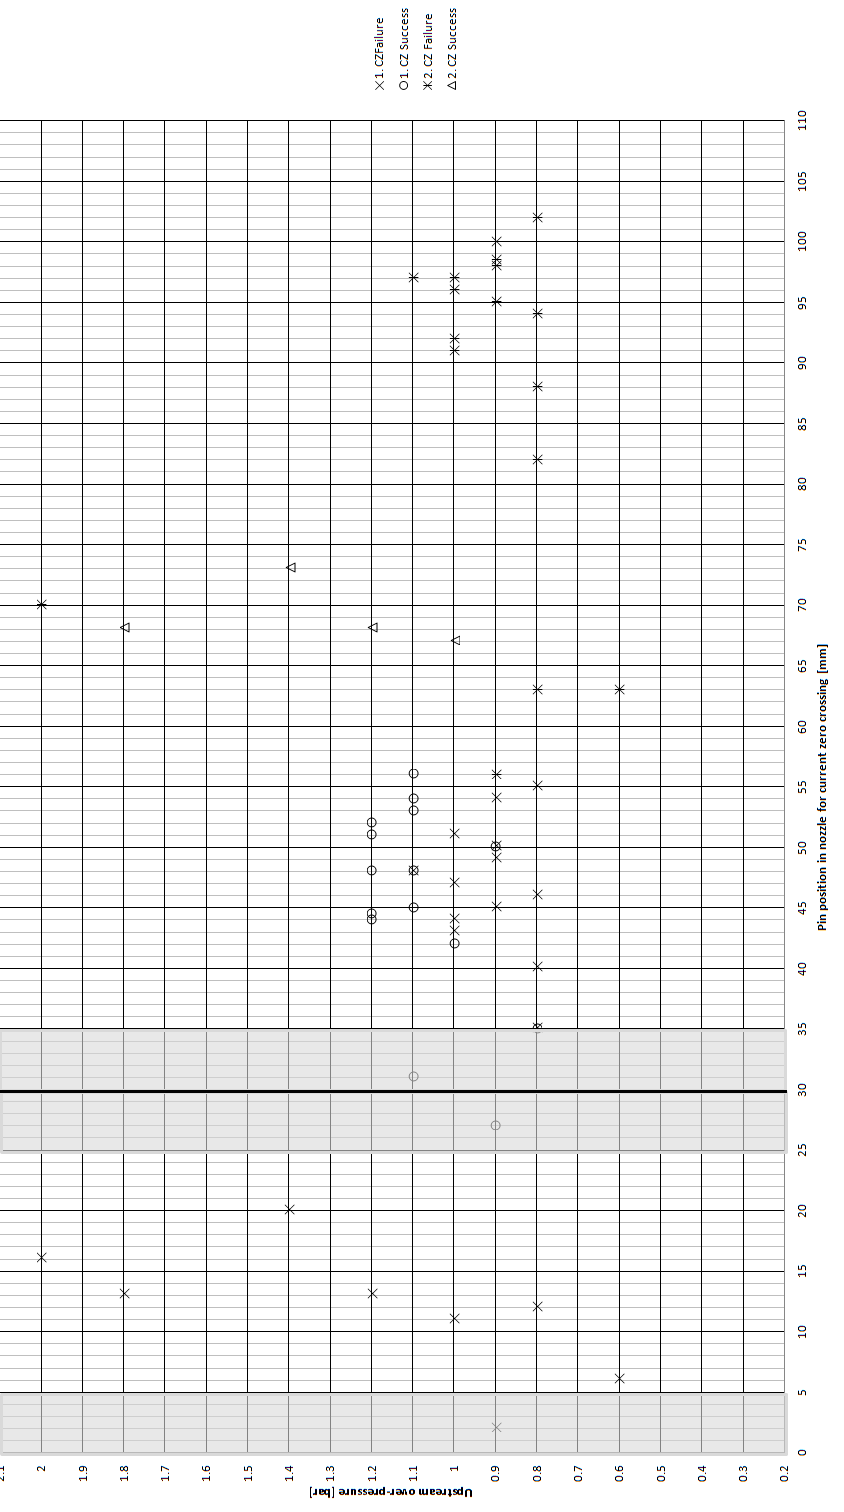
\includegraphics[scale=0.55]{Bilder/Results/rawData630AgeoA.png}
\caption{Raw data for geometry \textit{a} at 630 A, The grey areas are the boundary region where results was discarded for the success rate graphs. The black line indicates where the length of the nozzle.} \label{fig:rawData630AgeoA}
\end{figure}
\newpage

\begin{figure}[H]
\centering
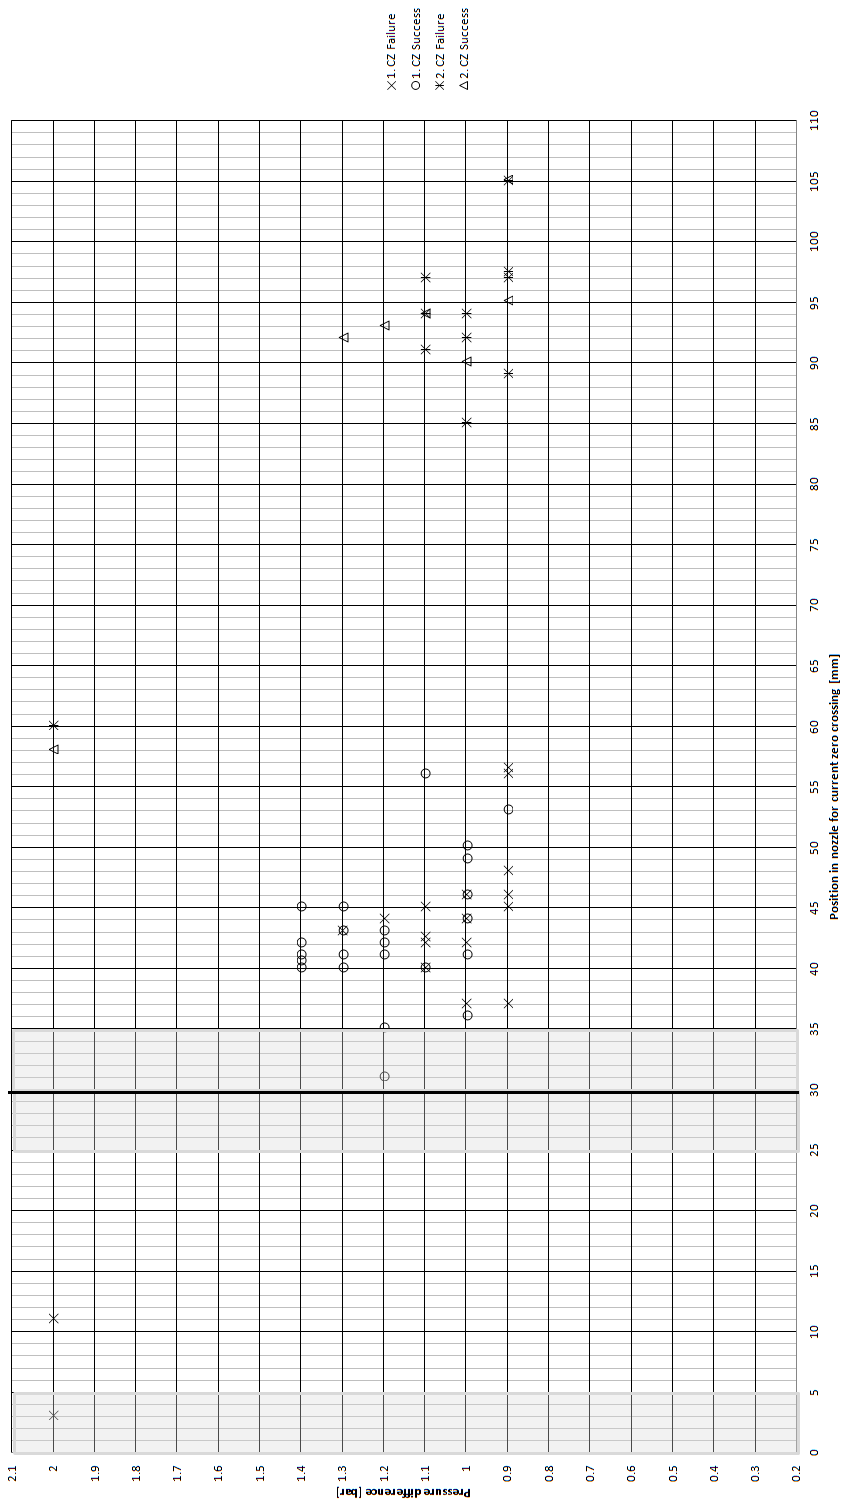
\includegraphics[scale=0.55]{Bilder/Results/rawData630AgeoB.png}
\caption{Raw data for geometry \textit{b} at 630 A, The grey areas are the boundary region where results was discarded for the success rate graphs. The black line indicates where the length of the nozzle.} \label{fig:rawData630AgeoB}
\end{figure}

\cleardoublepage
\section{Appendix: Previous relevant experiment} \label{app:PrevReleEx}
\makeatletter 
\renewcommand{\thefigure}{B.\@arabic\c@figure}
\makeatother

\makeatletter 
\renewcommand{\thetable}{B.\@arabic\c@table}
\makeatother

When investigating the interruption probability as in section \ref{sec:DiscIntChan} for the geometries presented in table \ref{tab:contGeoPara} it should be compared to the results obtained from past experiments. In the article "Current Interruption in Air for a Medium Voltage Load Break Switch" \cite{bib:CIAMVLBS} five geometries was tested. They all had the same diameter for the contact pin, but had different length and nozzle diameter as indicated in table \ref{tab:contactParaMVALBS}.
\begin{table} [H]
\center
\caption{Geometry parameters tested in:"Current Interruption in Air for a Medium Voltage Load Break Switch"}
\begin{tabular}{|c|c|c|c|c|c|}
\hline 
Geometry: & 1 & 2 & 3 & 4 & 5 \\ 
\hline 
D [mm] & 8 & 9 & 9 & 9 & 10 \\ 
\hline 
L [mm] & 30 & 15 & 30 & 60 & 30 \\ 
\hline 
d [mm] & 6 & 6 & 6 & 6 & 6 \\ 
\hline 
\end{tabular}
\label{tab:contactParaMVALBS}
\end{table}

\begin{figure}[H]
\centering
	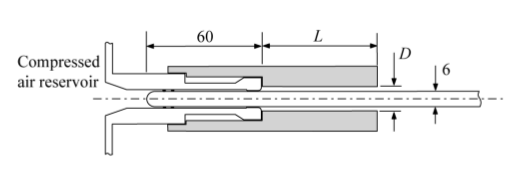
\includegraphics[scale=0.6]{Bilder/Discussion/paraDefine.png}
	\caption{Illustration of how the different parameters are defined  \cite{bib:CIAMVLBS}.}
	\label{fig:paraDefMVALBS}
\end{figure}

\begin{figure}[H]
  \centering
  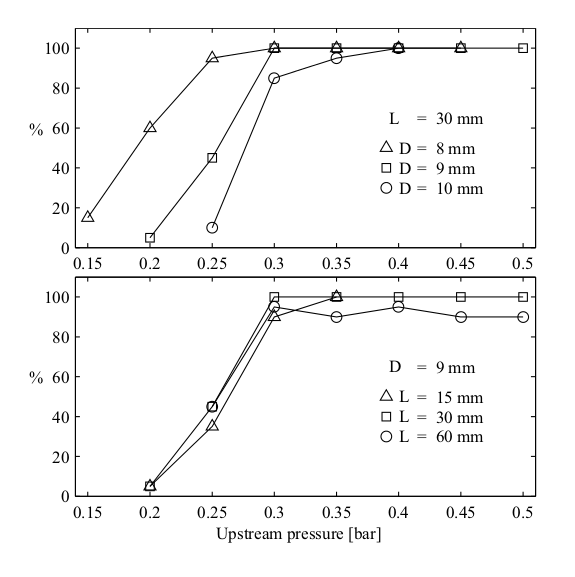
\includegraphics[scale=0.5]{Bilder/Discussion/percentSuccMVLBS.png}
  \caption{Percentage of successful interruptions as a function of the upstream pressure for all test series \cite{bib:CIAMVLBS}.}
  \label{fig:resultsCIMALBS}
\end{figure}

In figure \ref{fig:resultsCIMALBS} it can be observed that a short nozzle with a small diameter is preferred to obtain the lowest pressure for a series of successful interruptions. Besides the results from the article mentioned above, results from the article "Air Flow Investigation for a Medium Voltage Load Break Switch" \cite{bib:AFIMVLBA} should also be consulted, since the contact geometries used here have similarities to the ones used in the experiment conducted in this paper. The length of the nozzle was constant in this experiment, but both the pin and nozzle diameter was altered so that the ratio between them is approximately the same for all three geometries. If equation \eqref{eq:VolumetricFlow} is consulted it indicates that that the air velocity is the same for all three geometries. However the air velocity will depend the pin's position, and it will be different from when it is inside or outside the nozzle. This is because $v_\mathrm{{max}}$ will occur in the narrowest part of the geometry, this point varies between $A_\mathrm{{contact}}$ and $A_\mathrm{{ring}}$, depending on the pin's position. If compared to the geometries used in this paper the air flow is higher, but the air speed is usually smaller, due to the low upstream pressure needed for successful interruptions. In table \ref{tab:NinasGeo} the dimensions of the contact geometry for this experiment is presented and the results from the interruption test for all three currents and geometries, when the first CZ occurred outside the nozzle is illustrated in figure \ref{fig:ninaBryt}, where the magnitude of the current is illustrated with the line thickness and the diameter of the contacts is illustrated with a larger circle.

\begin{table}[H]
\center
\caption{Geometry parameters tested in:"Air Flow Investigation for a Medium Voltage Load Break Switch" \cite{bib:AFIMVLBA}.}
 \begin{tabular}{|c|c|c|c|c|}
\hline 
Geometry & D [mm] & d [mm] & $\frac{D}{d}$ & $\frac{A_\mathrm{{contact}}}{A_\mathrm{{contact,a}}}$ \\ 
\hline 
a & 8 & 6 & 1.33 & 1 \\ 
\hline 
b & 11 & 8 & 1.38 & 1.8 \\ 
\hline 
c & 13.6 & 10 & 1.36 & 2.8 \\ 
\hline 
\end{tabular} 
\label{tab:NinasGeo}
\end{table}

\begin{figure}[H]
  \centering
  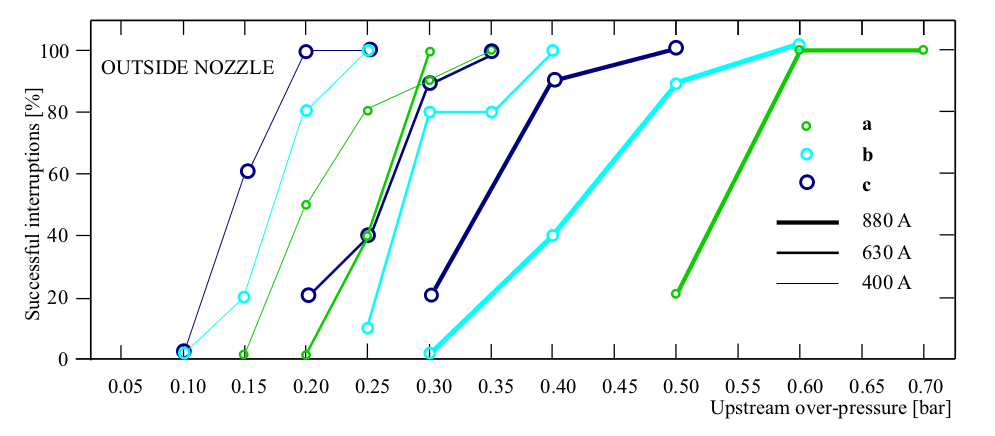
\includegraphics[scale=0.4]{Bilder/Discussion/ninaResults.png}
  \caption{Percentage of successful interruptions as a function of the upstream pressure for all test series outside the nozzle \cite{bib:AFIMVLBA}.}
  \label{fig:ninaBryt}
\end{figure}

It should be noted that the test series presented in figure \ref{fig:ninaBryt} only counted a successful interruption if the interruption occurred at the first CZ. For the results from the experiment conducted in this paper as presented in \ref{sec:interChance} a successful interruption was defined as a interruption at the first or second CZ. This might result in a higher success rate, however most of the interruptions for the experiment presented in this paper occurred at the first CZ if they succeeded, and therefore the results is comparable with the results presented in figure \ref{fig:ninaBryt}. In figure \ref{fig:ninaBryt2} the interruption results for the different geometries when CZ occurred inside the nozzle is indicated.

\begin{figure}[H]
  \centering
  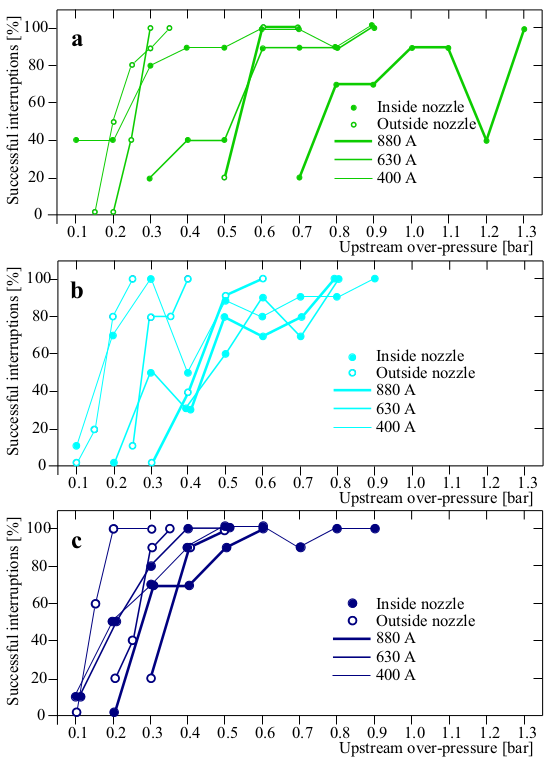
\includegraphics[scale=0.6]{Bilder/Discussion/testResultsNinaInside.png}
  \caption{Percentage of successful interruptions as a function upstream pressure for the different geometries when CZ occurs inside or outside the nozzle \cite{bib:AFIMVLBA}.}
  \label{fig:ninaBryt2}
\end{figure}

\end{document}
